%!TEX root=./LIVRO.tex


%%%%%%%%%%%%%%%%%%%%%%%%%%%%%%%%%%
%%% CHECK-LIST para FECHAMENTO %%% 
%%%%%%%%%%%%%%%%%%%%%%%%%%%%%%%%%%

%%%LATEX%%%%%%
%% # Arrumar o Sumário que está puxando ``Matemática'' do lugar errado e colocando a página errada 
%% # Arrumar identação dos boxes com espaço de parágrafo
%% # Resolver a protrusão do uso de \reduline com \linhas{4}

%%%EDIÇÃO%%%%%
%% # Conferir e limpar todas as ``Notes''.
%% # Conferir se todas as Atividades apresentam respostas discursivas 
%% (e não alternativas)
%% # Conferir se as imagens estão de acordo com o texto
%% # Conferir se todas as atividades, treinos etc. tem resposta (tem de ter, independentemente qual seja e onde entre)
%% Checar se imagem do último PDF entrou na posição correta
%% Contar um a um a ordem dos exercícios
%% Incluir créditos das imagens; Fábia e Felipe disseram que entram na página de créditos gerais, no início do volume


\chapter{O que dizem os números}
\markboth{Módulo 1}{}

\vspace*{-1cm}

\section*{Habilidades do SAEB}


\begin{itemize}
  \item Escrever números racionais (naturais de até 6 ordens, representação
fracionária ou decimal finita até a ordem dos milésimos) em sua
representação por algarismos ou em língua materna ou associar o registro
numérico ao registro em língua materna.

  \item Identificar a ordem ocupada por um algarismo ou seu valor posicional
(ou valor relativo) em um número natural de até 6 ordens.

  \item Comparar ou ordenar números racionais (naturais de até 6 ordens,
representação fracionária ou decimal finita até a ordem dos milésimos),
com ou sem suporte da reta numérica.

  \item Compor ou decompor números naturais de até 6 ordens na forma aditiva,
ou em suas ordens, ou em adições e multiplicações.

  \item Comparar diferentes sentenças de adições ou de subtrações de dois
números naturais.

  \item Determinar o número desconhecido que torna verdadeira uma igualdade
que envolve as operações fundamentais com números naturais de até 6
ordens.
\end{itemize}


\subsection{Habilidades da BNCC}

\begin{itemize}
\item EF03MA01, EF03MA04.
\end{itemize}

\conteudo{
Valor absoluto é o valor numérico do próprio algarismo, e o valor posicional, também conhecido como valor relativo, refere-se ao lugar que o algarismo ocupa no número, considerando a classe e a ordem. 
 
Exemplo.

No número 2.146, o algarismo 1 possui valor posicional ou
relativo igual a 100, pois ocupa a classe da centena, na 3ª ordem. 
Sendo assim, 1 x 100 = 100.

Com essas informações, é possível decompor o número 2.146, de acordo com a posição que cada algarismo ocupa no número: 2.146 = 2 x 1.000 + 1 x 100 + 4 x 10 + 6.

\vspace{1ex}
\noindent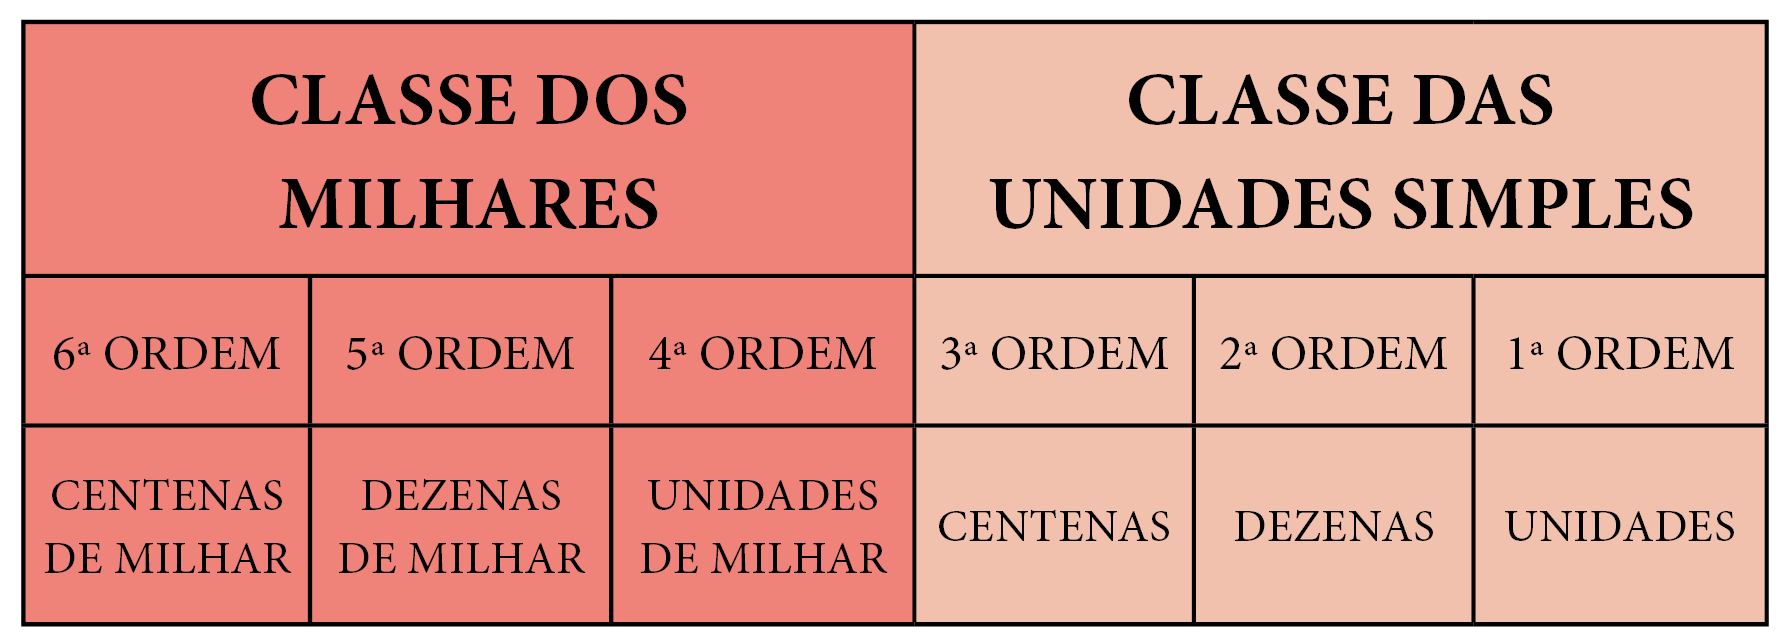
\includegraphics[width=\textwidth]{./media/image1.png}
}

\section*{Atividades}

\num{1} Vilma encontrou um pedaço de papel na sua bolsa. Nele, estava escrito o número a seguir:

\begin{figure}[htpb!]
\centering
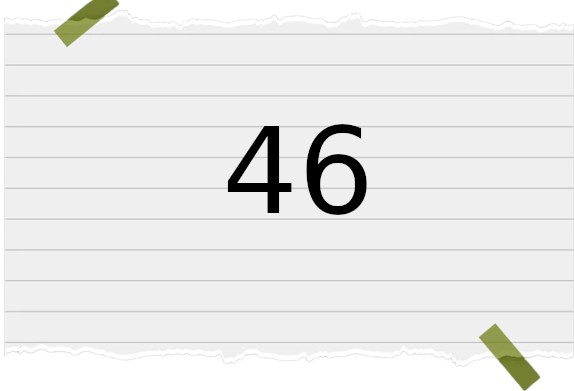
\includegraphics[width=.5\textwidth]{./media/image2.png}
\end{figure}

\pagebreak

\begin{escolha}
\item  Escreva o número 46 por extenso.
\reduline{Quarenta e seis.\hfill}
\linhas{1}

\item Calcule quantos grupos de 10 unidades é possível formar com o número 46.
\reduline{É possível formar 4 grupos de 10 unidades, e restam 6 que não são suficientes para formar outro grupo completo. Portanto, podemos expressar isso como 46 = 4 x 10 + 6\hfill}
\end{escolha}

\num{2} Arnaldo contou suas figurinhas. Com elas, ele montou 8 grupos com 10 figurinhas cada, e ainda adicionou mais quatro figurinhas ao total.

\begin{figure}[htpb!]
\centering
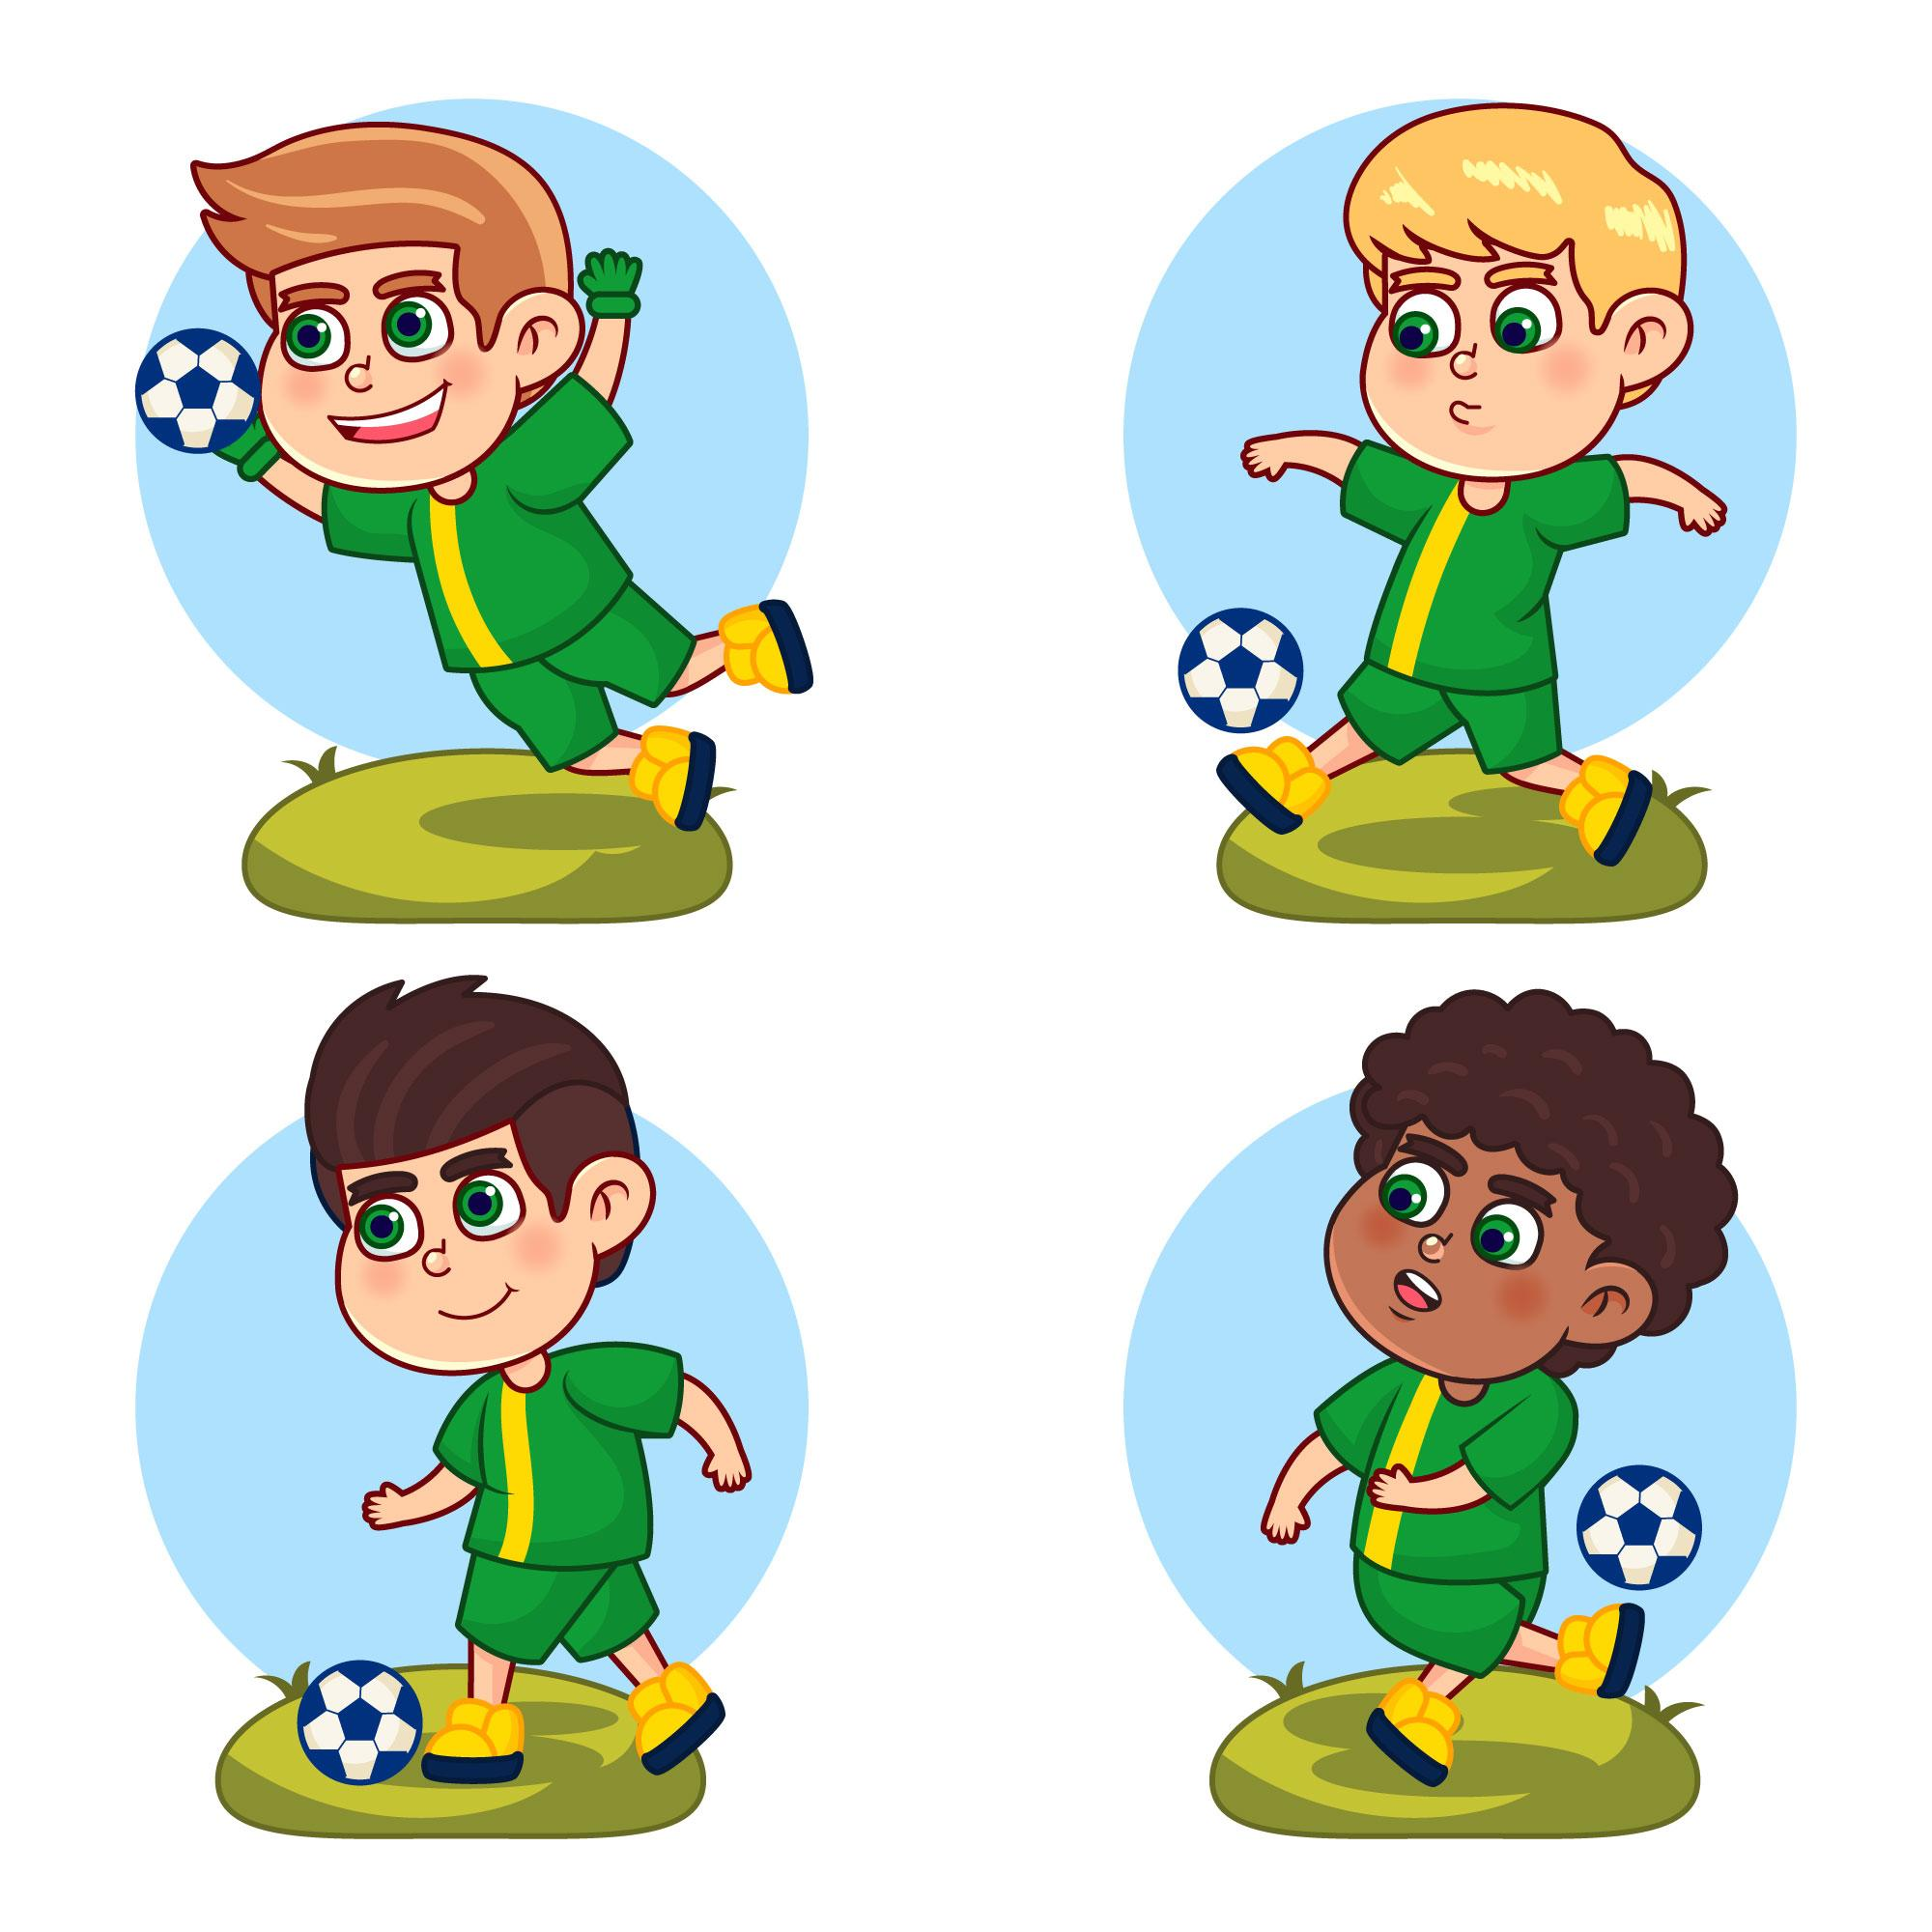
\includegraphics[width=.6\textwidth]{./media/image2a.jpg}
\end{figure}

\begin{escolha}
\item
  Calcule o número de figurinhas que Arnaldo possui.\\
\reduline{8 x 10 + 4 = 84\hfill}

\item  Escreva o número de figurinha que Arnaldo possui por extenso.\\
\reduline{Oitenta e quatro.\hfill}
\end{escolha}

\num{3} Treine sua criatividade, escrevendo:

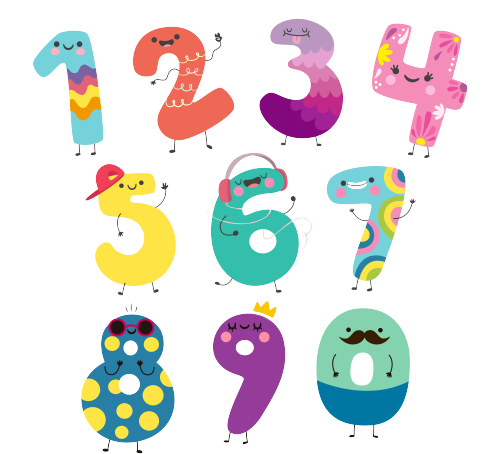
\includegraphics[width=\textwidth]{./media/image4a.png}

\begin{escolha}
\item Um número formado por três algarismos iguais.\\
\reduline{Resposta pessoal. Exemplo: 222.\hfill}

\item Um número formado por três algarismos no qual o 0 (zero) seja o terceiro algarismo.\\
\reduline{Resposta pessoal. Exemplo: 390.\hfill}

\item Um número formado por três algarismos diferentes.\\
\reduline{Resposta pessoal. Exemplo: 159.\hfill}

\item Um número com mais de três algarismos.\\
\reduline{Resposta pessoal. Exemplo: 1.477.\hfill}

\item Mostre os números que você criou para um colega e veja os números que ele criou.
\end{escolha}

\num{4} Escreva o número em algarismos ao lado de cada item e, em seguida, decomponha o número de acordo com o modelo.

\begin{myquote}
\begin{center}
\textbf{Cento e vinte e sete:} \textbf{127 = 100 + 20 + 7.}
\end{center}
\end{myquote}

\begin{escolha}
\item Trezentos e cinquenta e quatro.
\reduline{354 = 300 + 50 + 4.\hfill}

\item Duzentos e vinte e oito.
\reduline{228 = 200 + 20 + 8.\hfill}

\item Quatrocentos e setenta e seis.
\reduline{476 = 400 + 70 + 6.\hfill}
\end{escolha}

\num{5} Complete o quadro de acordo com a orientação.\bigskip

\noindent\begin{tabular}{llll}
\hline
\vspace{1.5em}
\begin{tabular}[c]{@{}l@{}}\textbf{Número escrito}\\ \textbf{por extenso}\end{tabular} & \begin{tabular}[c]{@{}l@{}}\textbf{Número escrito}\\ \textbf{em algarismos}\end{tabular} & \textbf{Número decomposto} \\ 
\hline
\vspace{1em}
Quinhentos e vinte e seis & \rosa{526} & \rosa{500} + 20 + 6 \\
\hline
\vspace{1em}
\rosa{Quatrocentos e trinta e cinco} & 435 & \rosa{400} + 30 + 5 \\
\hline
\vspace{1em}
\rosa{Oitocentos e trinta e dois} & \rosa{832} & 800 + 30 + 2 \\
\hline
\vspace{1em}
\rosa{Setecentos e vinte e nove} & \rosa{729} & 700 + 20 + 9 \\ 
\hline
\vspace{1em}
\rosa{Seiscentos e quarenta e um} & 641 & \rosa{600 + 40 + 1} \\ 
\hline
\end{tabular}

\pagebreak

\num{6} Durante a aula, Gabriel aprendeu a montar números utilizando o
material dourado. Ele montou o número abaixo:

%Produzir uma imagem semelhante a essa abaixo com 5 barras de 10 cubinhos cada e 9 cubinhos separados. Deixar a figura melhor apresentável e, se possível, numa cor parecida com o dourado.
\vspace{1.5em}

\begin{figure}[htpb!]
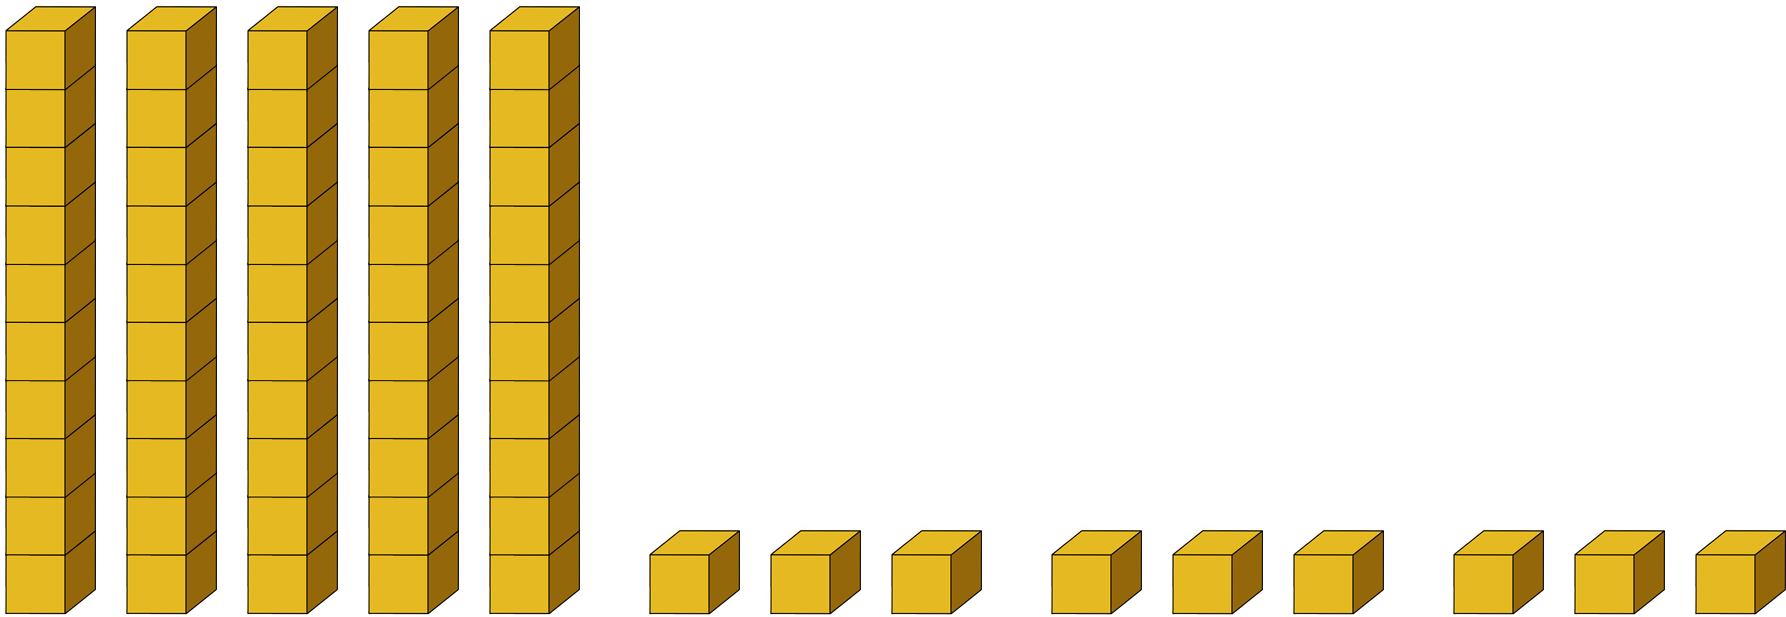
\includegraphics[width=\textwidth]{./media/image3.png}
\end{figure}
\vspace{1.5em}

\begin{escolha}
\item Qual é o número de cubos dourados representado na figura?
\reduline{Na figura, o número de cubos dourado é 59.\hfill}
\linhas{1}

\item Como o número montado por Gabriel pode ser decomposto?
\reduline{50 x 10 + 9 = 59.\hfill}
\linhas{1}
\end{escolha}

\num{7} Complete as informações abaixo de acordo com o que se pede. 

\begin{escolha}
\item
  Fernando tem 4 dezenas de lápis mais 2 unidades.

\begin{longtable}[]{@{}lll@{}}
\toprule
\textbf{Dezena} & \textbf{Unidade}\tabularnewline
\midrule
\endhead
&\tabularnewline
\bottomrule
\end{longtable}


Total de lápis que Fernando possui:
\reduline{4 x 10 + 2 = 42. Quarenta e dois lápis.\hfill}

\item Thiago tem 8 dezenas de bolinhas de gude mais 5 unidades.

\begin{longtable}[]{@{}lll@{}}
\toprule
\textbf{Dezena} & \textbf{Unidade}\tabularnewline
\midrule
\endhead
&\tabularnewline
\bottomrule
\end{longtable}

Total de bolinhas de gude que Thiago possui:
\reduline{8 x 10 + 5 = 85. Oitenta e cinco bolinhas de gude.\hfill}
\end{escolha}

\num{8} Realize a decomposição dos números indicados em cada item.

\begin{escolha}
\item 56: \reduline{5 x 10 + 6 = 56.\hfill}

\item 73: \reduline{7 x 10 + 3 = 73.\hfill}

\item 94: \reduline{9 x 10 + 4 = 94.\hfill}

\item 14: \reduline{1 x 10 + 4 = 14.\hfill}

\item 81: \reduline{8 x 10 + 1 = 81.\hfill}

\item 158: \reduline{1 x 100 + 5 x 10 + 8 = 158.\hfill}

\item 649: \reduline{6 x 100 + 4 x 10 + 9 = 649.\hfill}

\item 784: \reduline{7 x 100 + 8 x 10 + 4 = 784.\hfill}

\item 925: \reduline{9 x 100 + 2 x 10 + 5 = 925.\hfill}

\item 1.247: \reduline{1 x 1.000 + 2 x 200 + 4 x 10 + 7 = 1.247.\hfill}
\end{escolha}

\pagebreak

\num{9} Richard encontrou as seguintes peças de um material dourado:

\begin{figure}[htpb!]
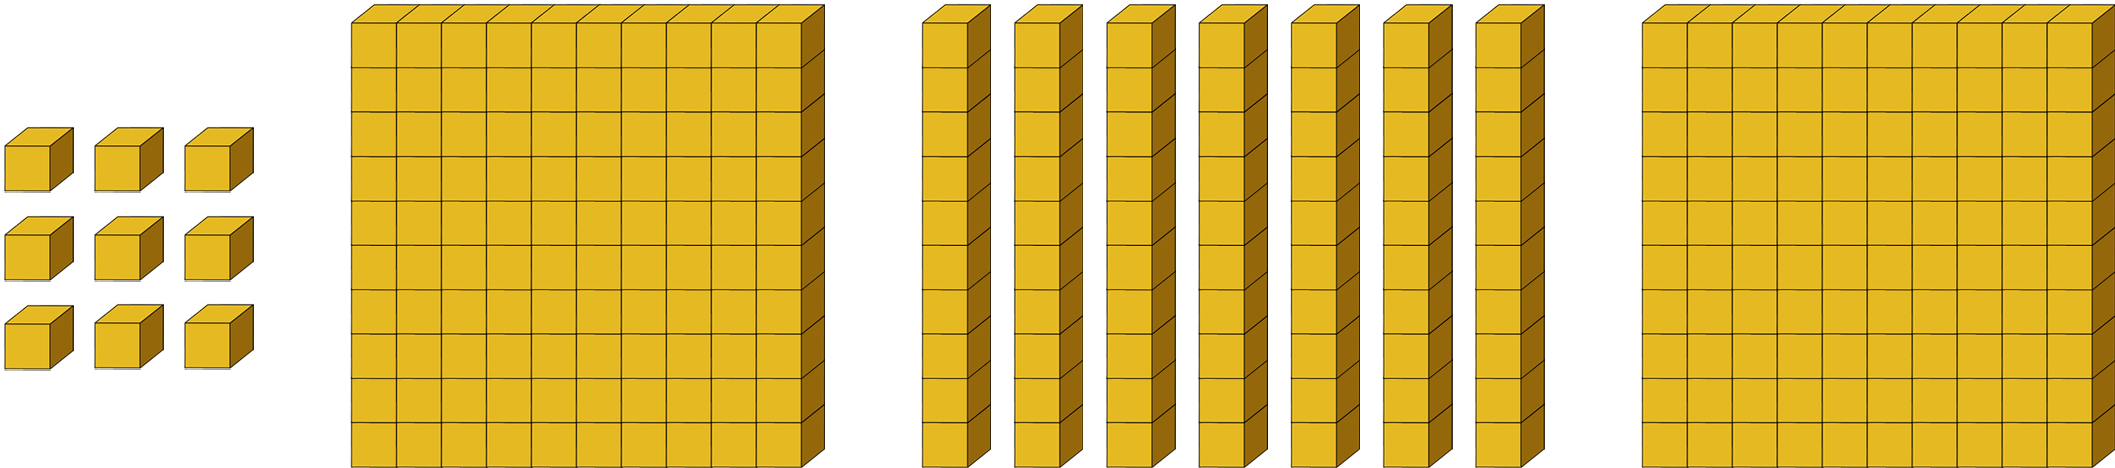
\includegraphics[width=\textwidth]{./media/image4.png}
\end{figure}

Somando todas as peças, qual o maior número que Richard pode representar? 
\reduline{2 x 100 + 7 x 10 + 9 = 279.\hfill}
\linhas{3}

Após encontrar o número, escreva-o por extenso.
\reduline{Duzentos e setenta e nove.\hfill}
\linhas{1}

\num{10} Monte os números compostos e escreva-os nos locais correspondentes.

\begin{escolha}
\item 5 centenas e 4 unidades:
\reduline{504.\hfill}

\item 7 dezenas e 2 unidades:
\reduline{2.\hfill}

\item 9 centenas, 5 dezenas e 6 unidades:
\reduline{956.\hfill}

\item 2 centenas, 6 dezenas e 3 unidades:
\reduline{263.\hfill}

\item 4 dezenas e 8 unidades
\reduline{48.\hfill}

\item 1 unidade de milhar, 7 centenas, 1 dezena e 9 unidades
\reduline{1.719.\hfill}

\end{escolha}

\begin{comment}
\num{11} Ligue o número em algarismos da coluna 1 
à representação correspondente escrita por extenso na coluna 2.

\begin{figure}[htpb!]
\centering
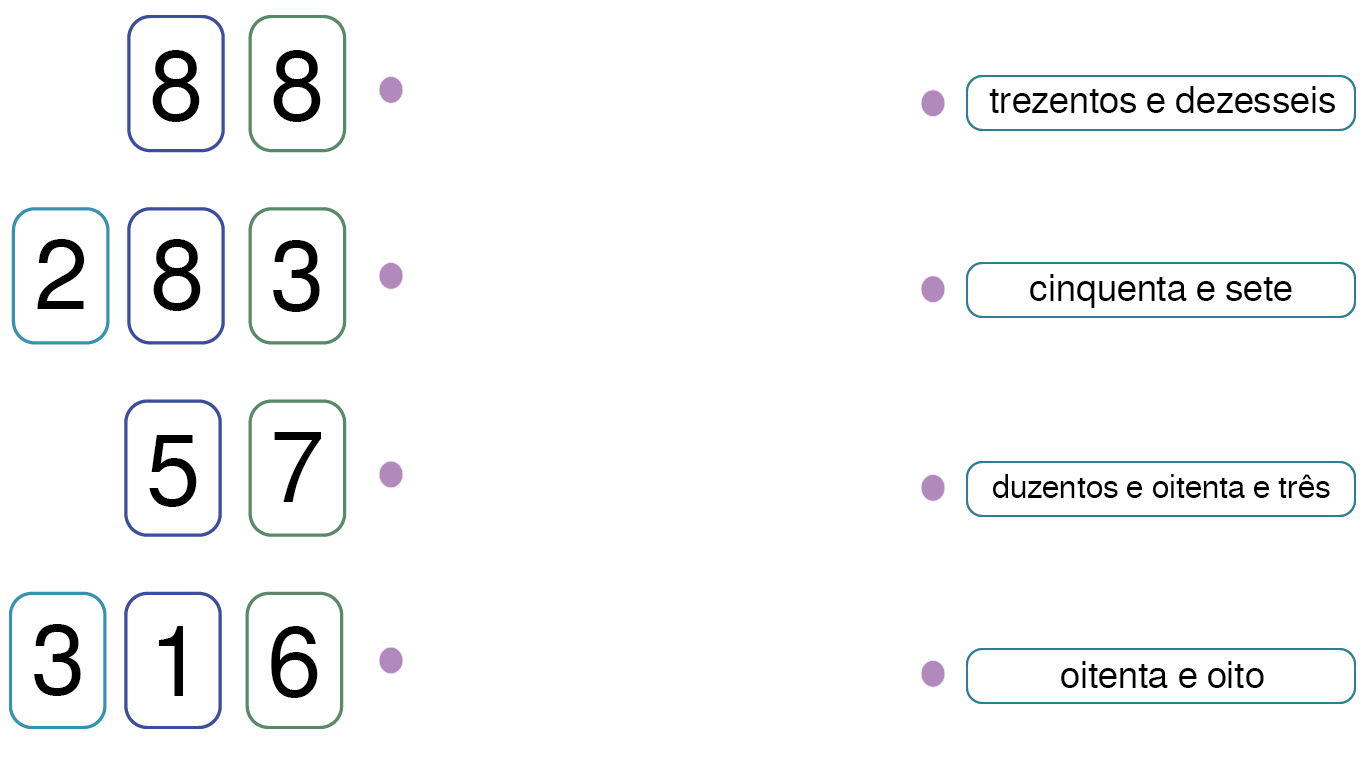
\includegraphics[width=\textwidth]{./media/image5.png}
\end{figure}

\coment{88 (oitenta e oito); 283 (duzentos e oitenta e três); 57 (ciquenta e sete); e 316 (a trezentos e dezesseis).}
\end{comment}

\num{11} Leia o enunciado e responda ao que se pede. 

\vspace{1em}

\begin{figure}[htpb!]
\centering
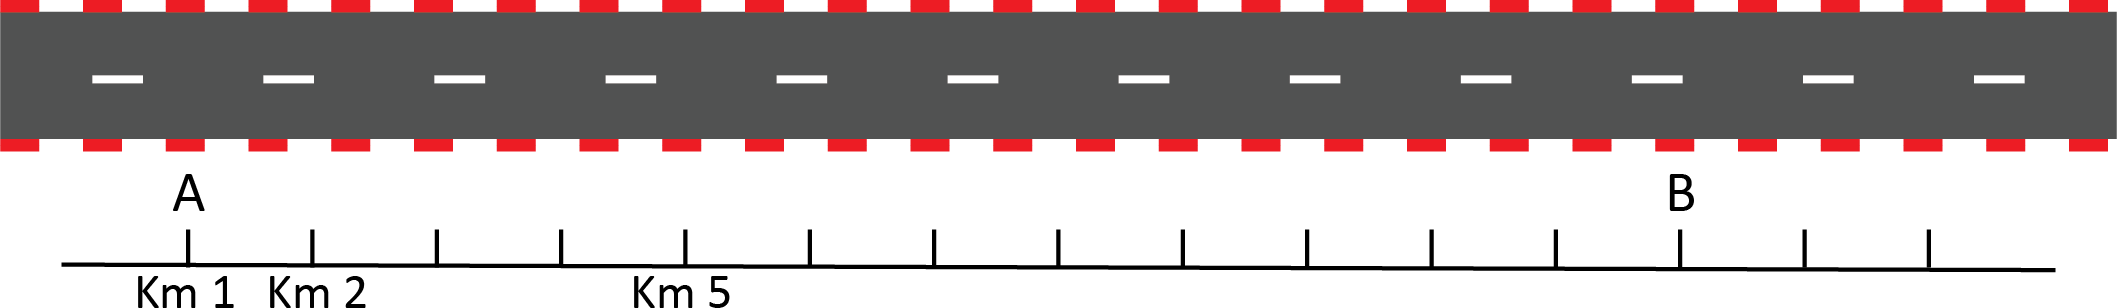
\includegraphics[width=\textwidth]{./media/image6.png}
\end{figure}

\vspace{1em}

Felipe desenhou uma linha reta para representar a distância de uma corrida de A até B. Ele também dividiu essa reta em intervalos de 1 km. 

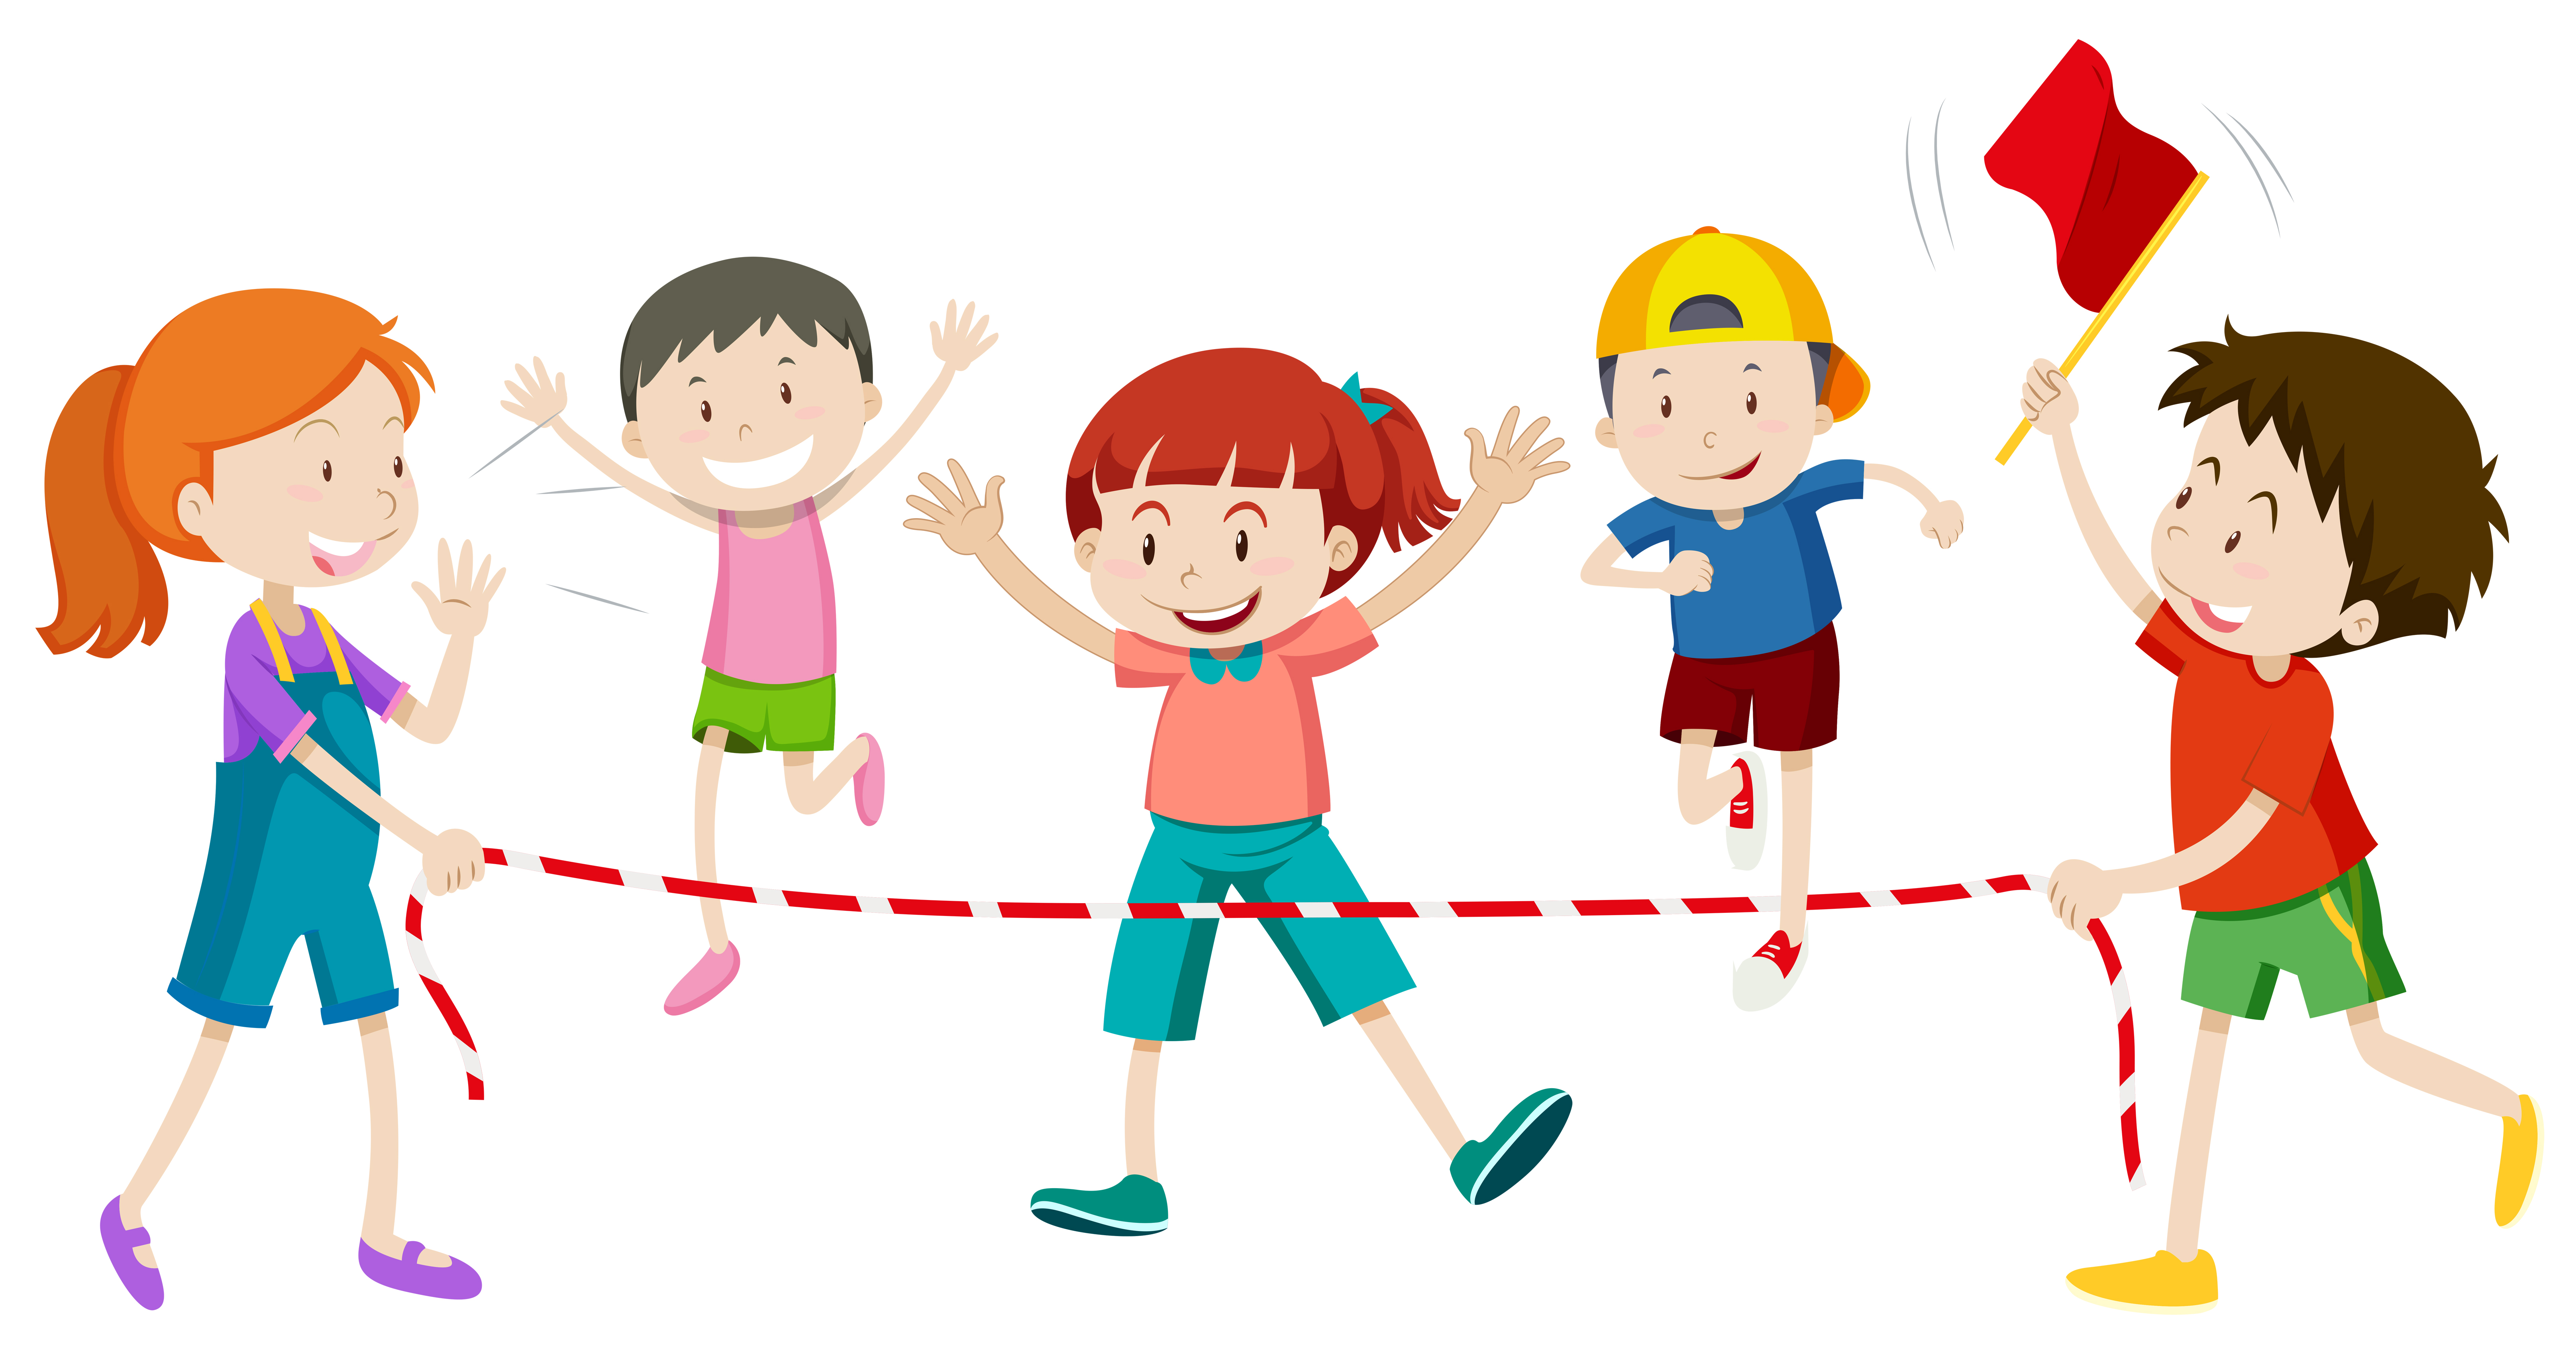
\includegraphics[width=\textwidth]{./media/image6a.jpeg}



\begin{escolha}
\item Calcule em que ponto Felipe parou na marcação, sabendo que ele completou a corrida.\\
\reduline{Km 12.\hfill}
\linhas{3}
\end{escolha}


\begin{comment}
%\sidetext{Felipe saiu do ponto A, que está em cima da marcação do quilômetro 0, e chegou ao
%ponto B, que está a 12 marcações de distância do ponto, podemos concluir
%que ele parou no km 12; ou seja, percorreu 12 km.

%Explore com os alunos a colocação dos números na reta numérica, considerando
%que é um conceito essencial em outros assuntos.}

\num{13} A bolas representadas na imagem abaixo fazem parte do jogo de sinuca. Observe os números e responda ao que se pede:

\begin{figure}[htpb!]
\centering
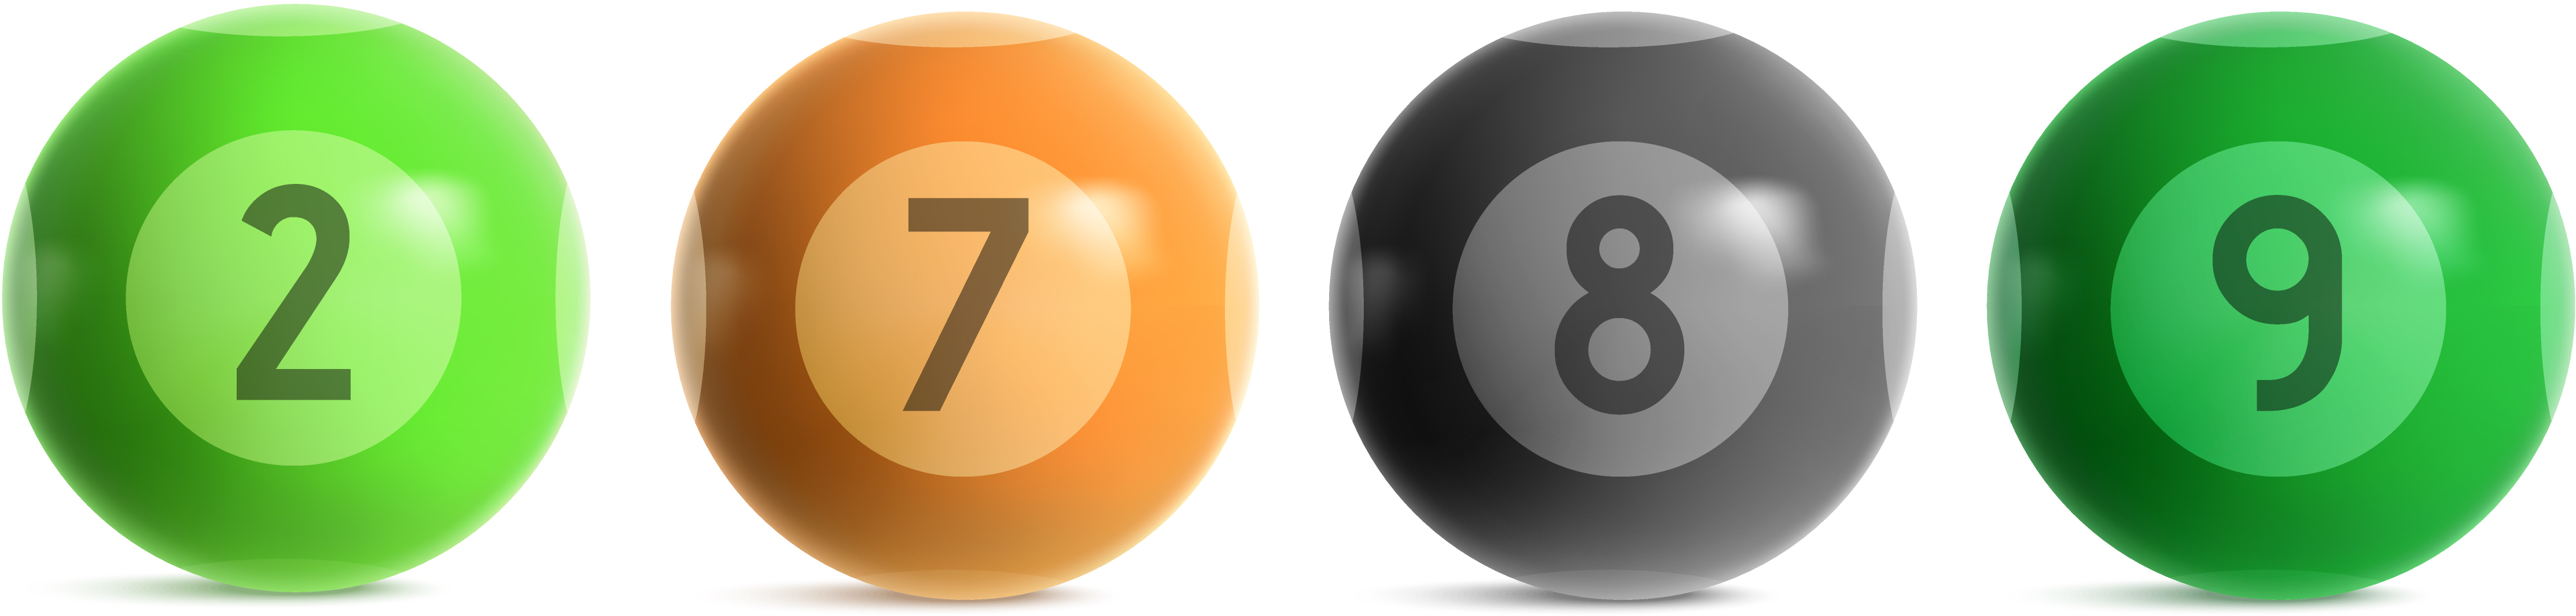
\includegraphics[width=\textwidth]{./media/image7.png}
\end{figure}
%NOTE. ICO. Montar na seguinte ordem ``7 9 2 8''.


\begin{escolha}
\item Qual a bola de maior número?
\reduline{A bola de número é a de número 9 (nove).\hfill}

\item Usando os números das bolas, forme o menor número de três ordens. 
\reduline{O número é 278 (duzentos e setenta e oito).\hfill}

\item Usando os números das bolas, forme o maior número par.
\reduline{9.872 (nove mil oitocentos e setenta e dois).\hfill}

\end{escolha}

%\coment{Explore mais exemplos com os alunos para estimular a criatividade
%e a formação de números.}
\end{comment}

\pagebreak

\section*{Treino}

\num{1} Amanda estava brincando no escritório de seu pai quando
encontrou um pedaço de papel com uma anotação: faturamento diário: 734 reais.

\begin{figure}[htpb!]
\centering

\includegraphics[width=0.6\textwidth]{./media/image6b.png}
\end{figure}

Lembrando-se das aulas de matemática, ela resolveu decompor o número escrito
no papel. Qual é a decomposição que Amanda deve fazer desse
número?

\begin{escolha}
\item
  700 + 30 + 4.
\item
  70 + 3 + 4.
\item
  700 + 40 + 3.
\item
  70 + 300 + 4.
\end{escolha}

\pagebreak

\num{2} Na reta numérica a seguir, o ponto P representa o número 540, e o ponto U representa o número 590.

\begin{figure}[htpb!]
\centering
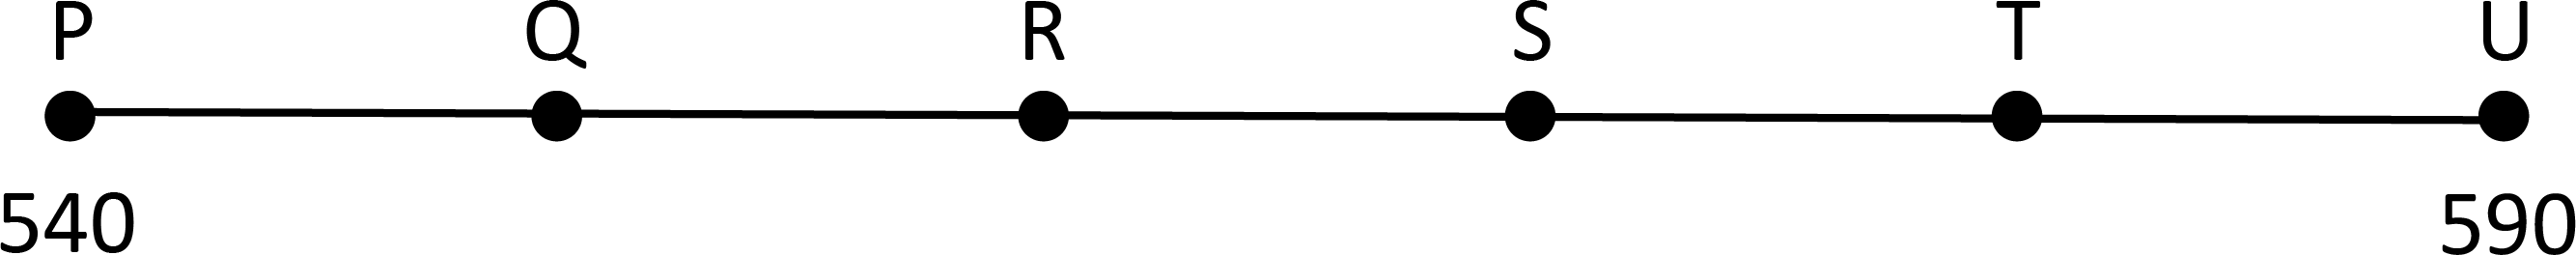
\includegraphics[width=\textwidth]{./media/image8.png}
\end{figure}

Indique o ponto correspondente à representação do número 570, sabendo que a
distância entre dois pontos consecutivos é de 10 unidades.

\begin{escolha}
  \begin{multicols}{2}
\item
  Q.
\item
  R.
\item
  S.
\item
  T.
  \end{multicols}
\end{escolha}

\num{3} Utilizando o material dourado, Ana Letícia montou um número.

\begin{figure}[htpb!]
\centering
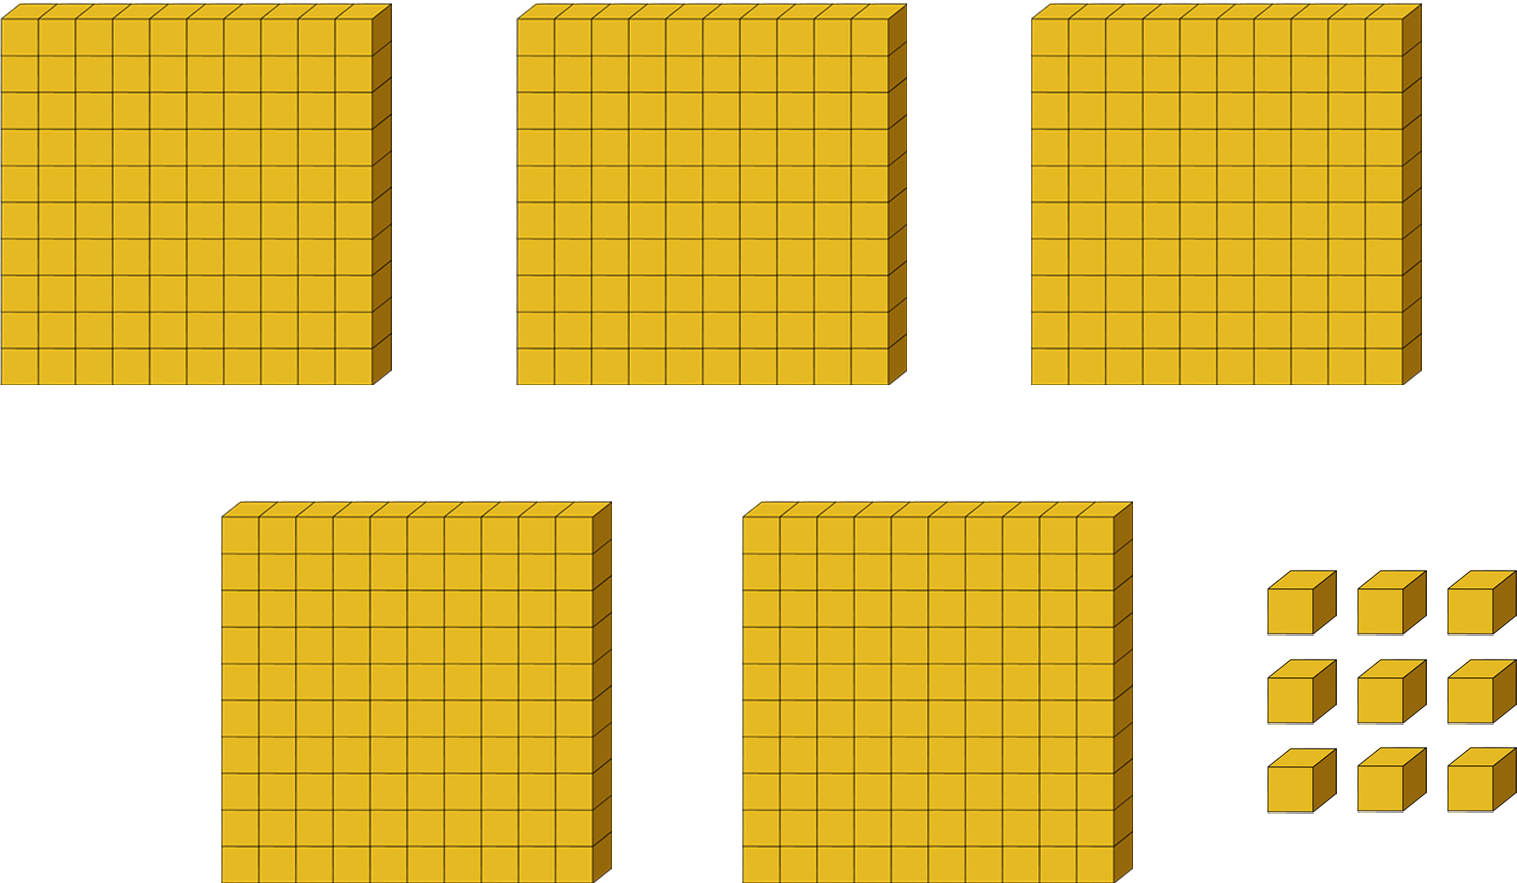
\includegraphics[width=\textwidth]{./media/image9.png}
\end{figure}

Qual é o número representado por Ana Letícia? 

\begin{escolha}
  \begin{multicols}{2}
\item
  59.
\item
  159.
\item
  509.
\item
  1.509.
  \end{multicols}
\end{escolha}

\chapter{Cálculos}
\markboth{Módulo 2}{}

\section*{Habilidades do SAEB}

\begin{itemize}
\item Calcular o resultado de adições ou subtrações, envolvendo números
naturais de até 6 ordens.

\item Calcular o resultado de multiplicações ou divisões, envolvendo números
naturais de até 6 ordens.

\item Associar o quociente de uma divisão com resto zero de um número
natural de até 6 ordens por 2, 3, 4, 5 e 10 às ideias de metade, terça,
quarta, quinta e décima parte.

\item Resolver problemas de adição ou de subtração, envolvendo números
naturais de até 6 ordens, com os significados de juntar, acrescentar,
separar, retirar, comparar ou completar.

\item Resolver problemas de multiplicação ou de divisão, envolvendo números
naturais de até 6 ordens, com os significados de formação de grupos
iguais (incluindo repartição equitativa e medida), proporcionalidade ou
disposição retangular.
\end{itemize}

\subsection{Habilidades da BNCC}

\begin{itemize}
\item EF03MA06, EF03MA07, EF03MA08.
\end{itemize}

%\conteudo{ Assim como todos os conteúdos que envolvem as quatro operações básicas, este módulo é essencial e seu estudo deve ser feito com tempo para bastante treino. Relembre com os alunos cada detalhe e os algoritmos de adição, subtração, multiplicação e divisão, dando  ênfase à divisão, que geralmente é o maior desafio enfrentado pelos alunos. }
\pagebreak

\conteudo{
\begin{itemize}
\item [ ] \textsc{Adição}
\end{itemize}
\begin{center}
\noindent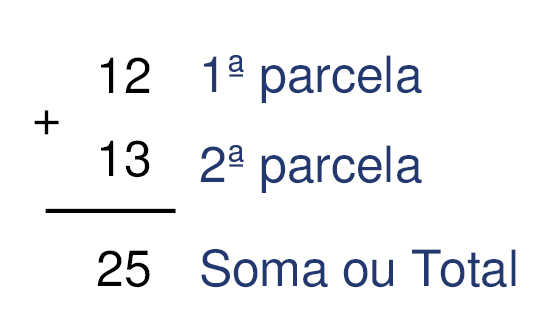
\includegraphics[width=.3\textwidth]{./media/image10.png}
\end{center}

\begin{itemize}
\item [ ] \textsc{Subtração}
\end{itemize}
\begin{center}
\noindent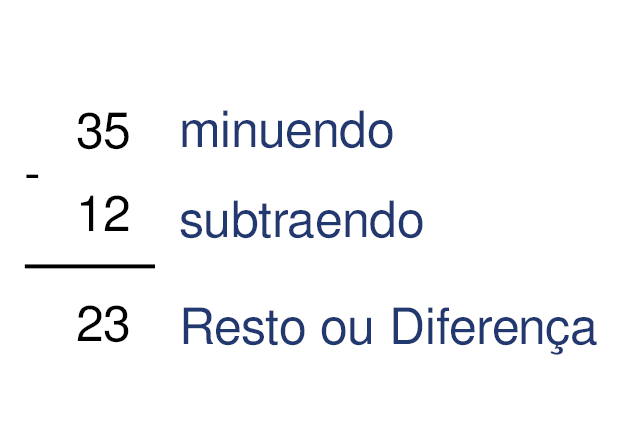
\includegraphics[width=.3\textwidth]{./media/image11.png}
\end{center}

\begin{itemize}
\item [ ] \textsc{Multiplicação}
\end{itemize}
\begin{center}
\noindent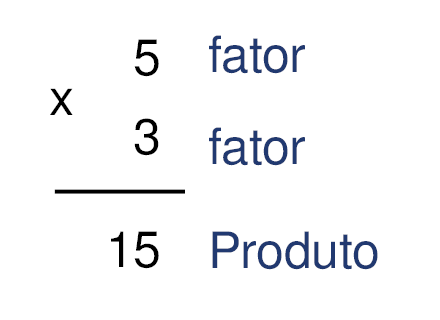
\includegraphics[width=.3\textwidth]{./media/image12.png}
\end{center}

\begin{itemize}
\item [ ] \textsc{Divisão}
\end{itemize}
\begin{center}
\noindent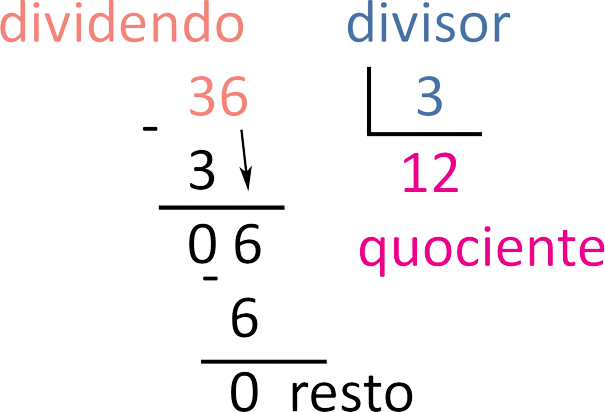
\includegraphics[width=.3\textwidth]{./media/image13.png}
\end{center}
}

\pagebreak 

\section*{Atividades}

\num{1} Adicione ou subtraia para obter o número desejado.

\begin{escolha}

\item
  Transforme 262 em 362.\\
\reduline{Adicionar 100.\hfill}
\linhas{2}

\item
  Transforme 1.100 em 1.000.\\
\reduline{Subtrair 100.\hfill}
\linhas{2}

\item
  Transforme 238 em 239.\\
\reduline{Adicionar 1.\hfill}
\linhas{2}
\end{escolha}

\num{2} Utilize os sinais menor que (\textbf{\textless{}}), maior que (\textbf{\textgreater{}}) ou igual a
(\textbf{=}) em cada situação para comparar as quantidades representadas.\bigskip

\begin{minipage}{.5\textwidth}
\begin{escolha}
\item
  7 \reduline{Menor que, \textless{}} 14
\item
  21 \reduline{Maior que, \textgreater{}} 5
\item
  1 + 3 \reduline{Igual a, =} 2 + 2
  \end{escolha}
  \end{minipage}
\begin{minipage}{.5\textwidth}
  \begin{escolha}[start=4]
\item
  5 + 2 \reduline{Maior que, \textgreater{}} 7 -- 1
\item
  20 -- 1 \reduline{Igual a, =} 19
\item
  Treze \reduline{Menor que, \textless{}} quinze
\end{escolha}
\end{minipage}

\pagebreak

\num{3} Ligue a operação na coluna 1 ao seu resultado na coluna 2.

\begin{multicols}{2}
84 + 12

60 -- 23

67 -- 58

50 -- 2 x (5 + 15) + 2

2 + 8 -- 2 x (1 + 2)

37

9

96

4

12
\end{multicols}
%\coment{Explore ao máximo com os alunos o conceito de quais operações devem ser realizadas primeiro e, assim, ajude na fixação desse conceito.
\coment{Respostas: 84 + 12 = 96; 60 - 23 = 37; 67 - 58 = 9; 50 - 2 x (5 + 15) + 2 = 50 - 40 + 2 = 12; 2 + 8 - 2 x (1 + 2) = 2 + 8 - 6 = 4}

\num{4} Observe atentamente a figura dada e, em seguida, responda ao que se pede em cada item.


\begin{figure}[htpb!]
\centering
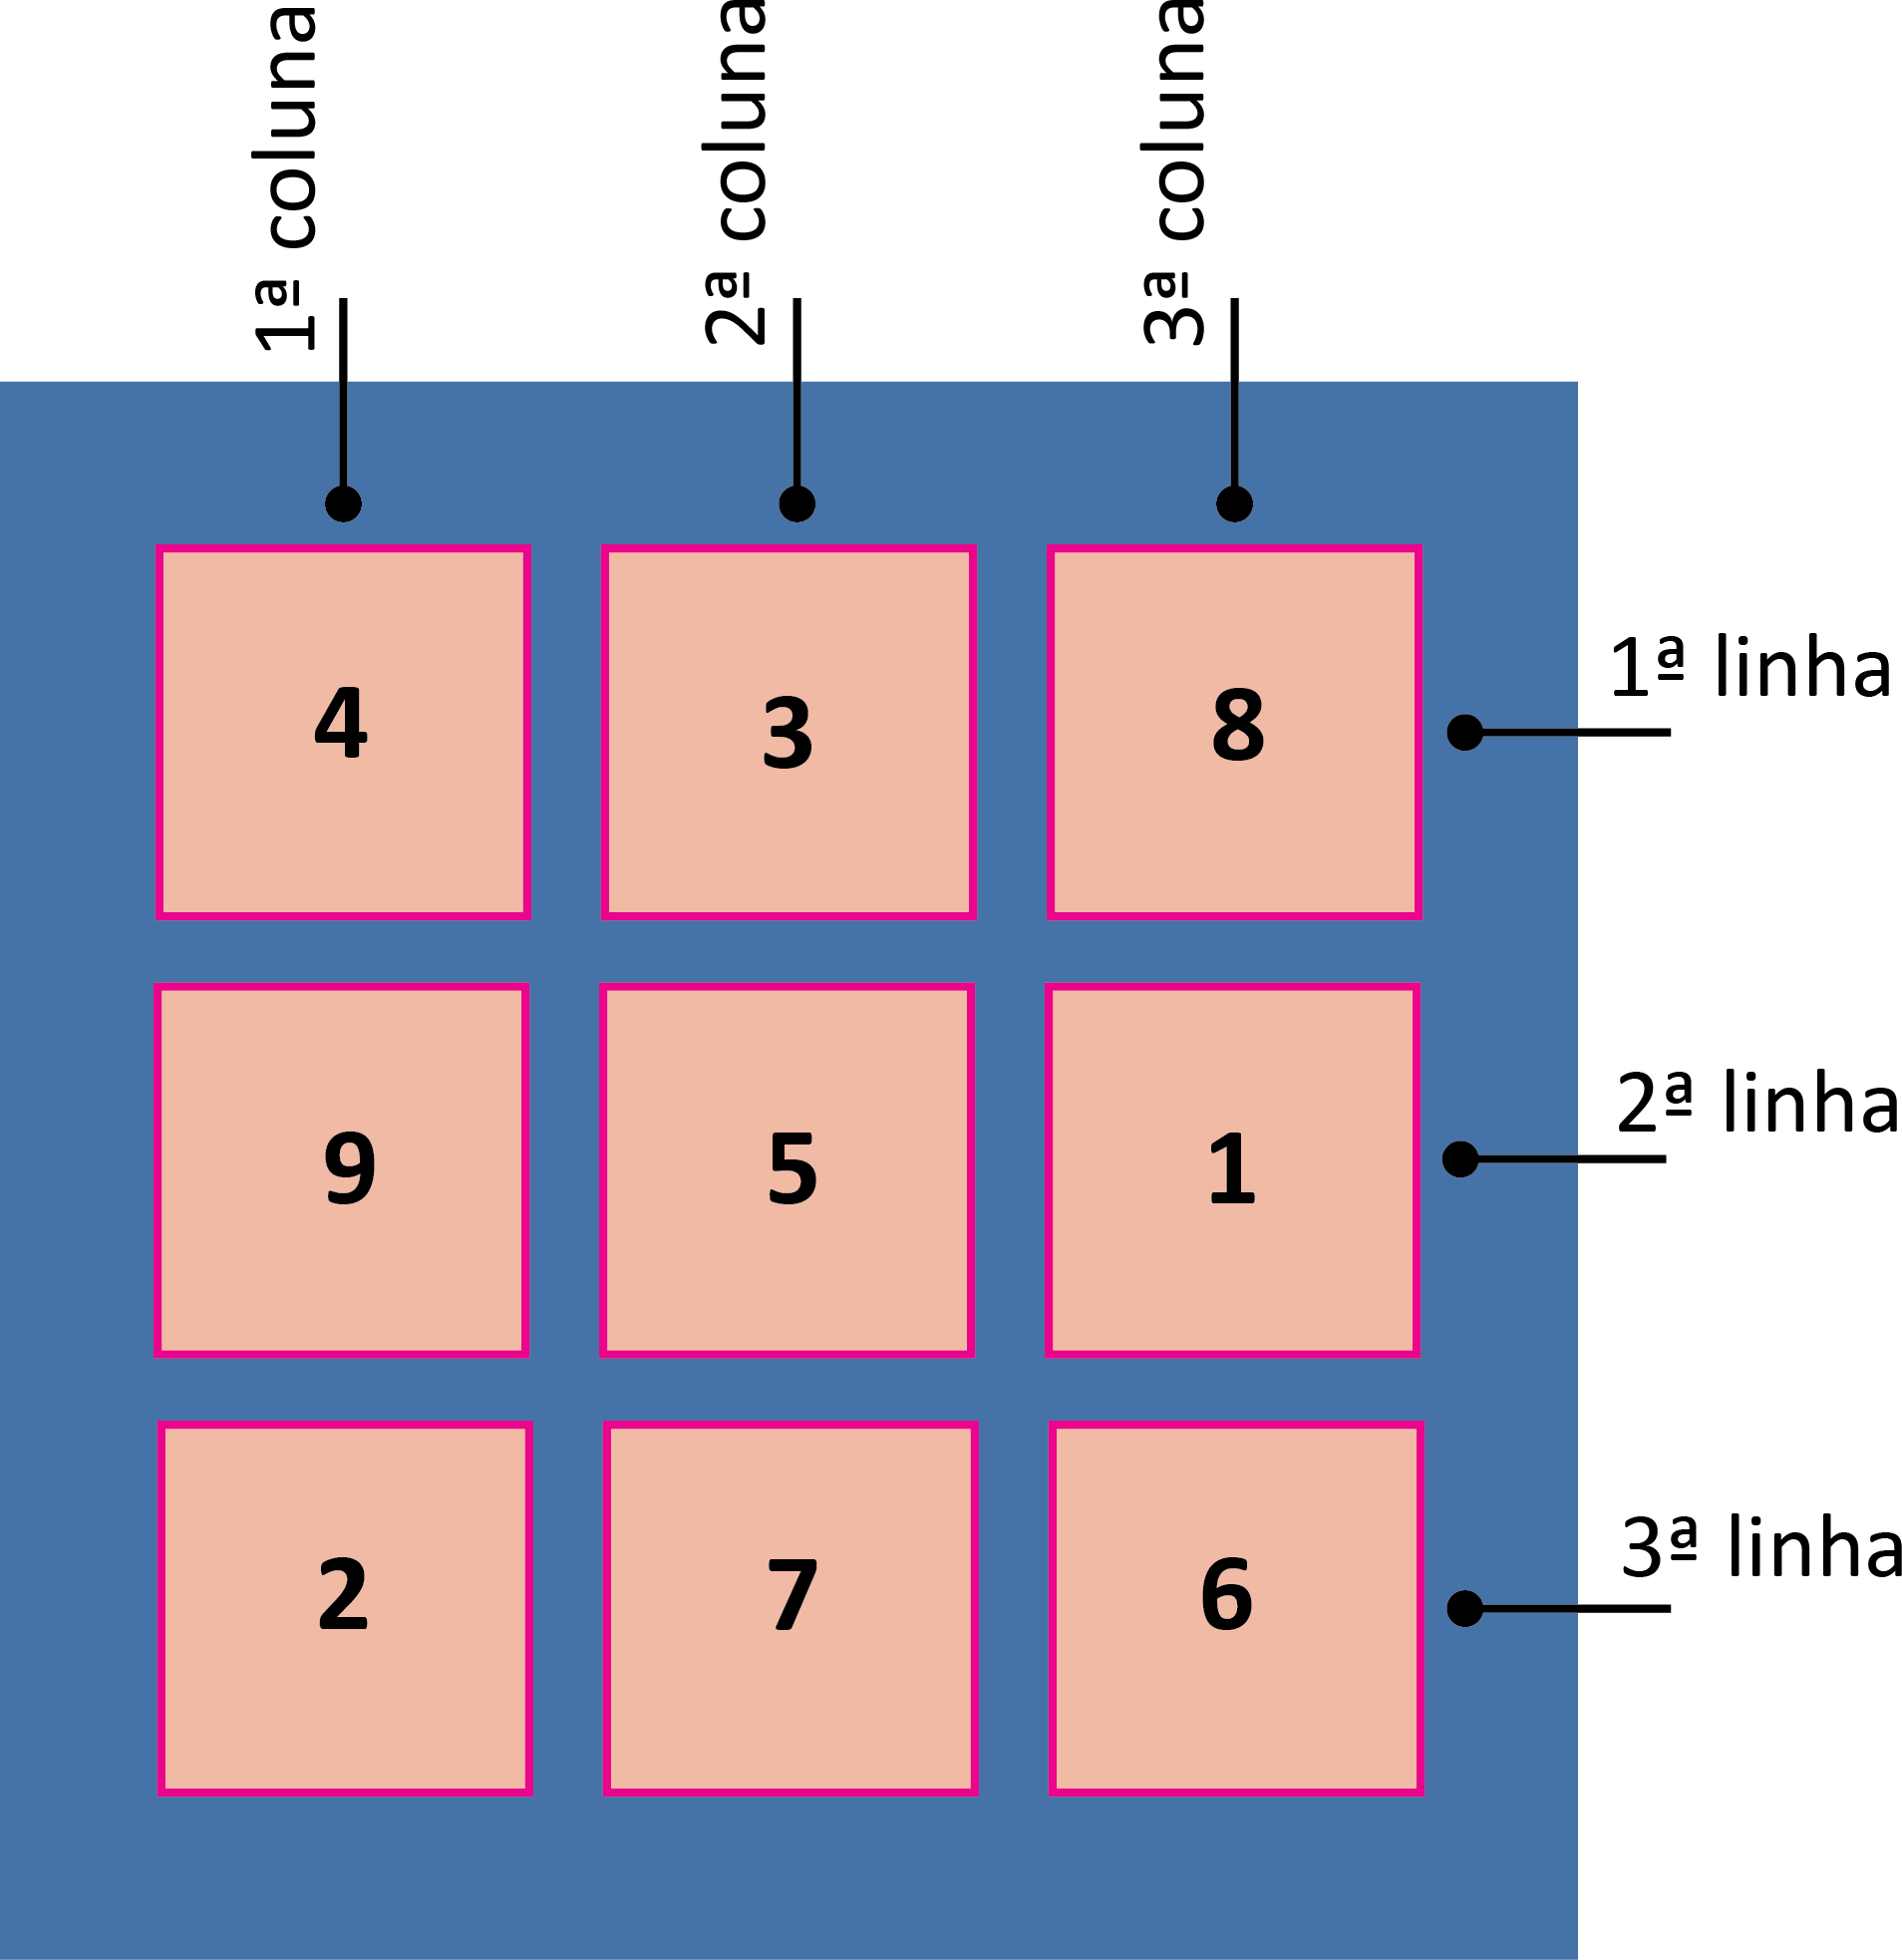
\includegraphics[width=.5\textwidth]{./media/image14.png}
\end{figure}

\begin{escolha}
\item Calcule a soma de todos os números que estão na 1ª coluna.
\reduline{4 + 9 + 2 = 15.\hfill}
\linhas{1}

\pagebreak
\item Calcule a soma de todos os números que estão na 2ª coluna.
\reduline{3 + 5 + 7 = 15.\hfill}
\linhas{1}

\item Calcule a soma de todos os números que estão na 3ª coluna.
\reduline{8 + 1 + 6 = 15.\hfill}
\linhas{1}

\item O que você percebe ao comparar os resultados das somas dos números de cada coluna?
\reduline{O resultado de todas as somas apresentam resultado igual a 15.\hfill}
\linhas{1}

\item Calcule a soma dos números que estão na 1ª linha.
\reduline{4 + 3 + 8 = 15.\hfill}
\linhas{1}

\item Calcule a soma dos números que estão na 2ª linha.
\reduline{9 + 5 + 1 = 15.\hfill}
\linhas{1}

\item Calcule a soma dos números que estão na 3ª linha.
\reduline{2 + 7 + 6 = 15.\hfill}
\linhas{1}

\item O que você percebe quando compara os resultados da soma dos números de cada linha?
\reduline{O resultado de todas as somas apresentam resultado igual a 15.\hfill}
\linhas{1}
\end{escolha}

\num{5} Vicente vendeu 6 sorvetes de chocolate, 8 de morango, 3
de groselha e 5 de creme. Quantas unidades de sorvete Vicente vendeu?
\begin{figure}[htpb!]
\centering
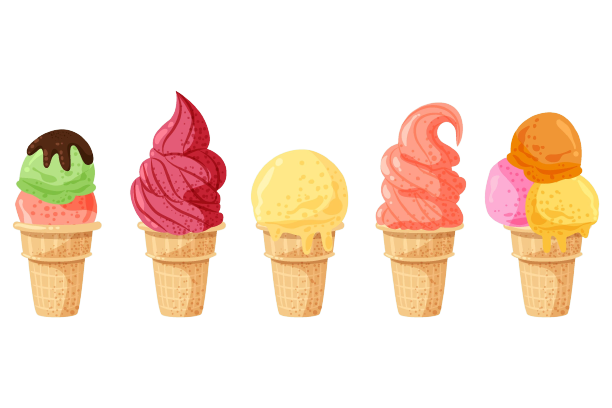
\includegraphics[width=.5\textwidth]{./media/image14a.png}
\end{figure}

\reduline{Vicente vendeu 6 + 8 + 3 + 5 = 22. \hfill}
\linhas{1}

\num{6} A receita de um bolo pede para colocar 260 g de
farinha de trigo e misturar com ovos, açúcar e leite. 
Em seguida, solicita o acréscimo de mais 135 g de farinha de trigo. 
Calcule a quantidade total de farinha utilizada nesta receita?

\begin{figure}[htpb!]
\centering
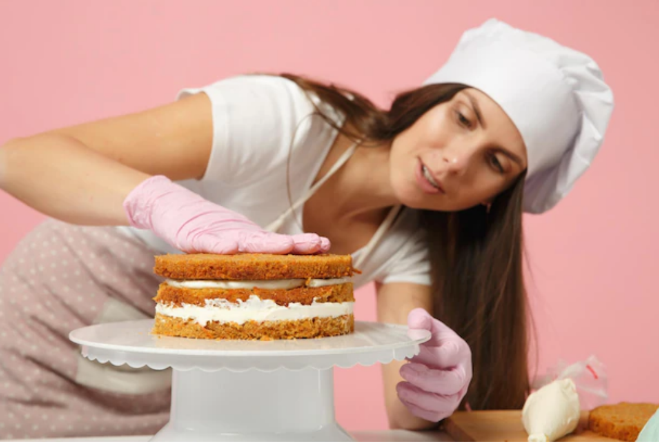
\includegraphics[width=.5\textwidth]{./media/image15.png}
\end{figure}
\reduline{260 + 135 = 395 g.\hfill}
\linhas{3}

\num{7} Raquel adora confeitaria. Por isso, 
decidiu começar uma pequena empresa de doces para festas. 
Para o próximo final de semana, ela recebeu a seguinte 
encomenda por mensagem de texto em seu celular:

\begin{myquote}
\centering
\textbf{Encomenda para a festa da Maria}

\begin{itemize}
\centering
\item [ ] 275 brigadeiros

\item [ ] 165 beijinhos

\item [ ] 245 cajuzinhos
\end{itemize}
\end{myquote}

Calcule o total de unidades de doces que Raquel terá que fazer para entregar essa encomenda.
\reduline{275 + 165 + 245 = 685.\hfill}
\linhas{3}

\num{8} Complete o quadro, transformando as adições em multiplicações. Em seguida, encontre o resultado.

\begin{longtable}[]{@{}lll@{}}
\toprule
\hline
\vspace{1ex}
\textbf{Adição de parcelas iguais} & \textbf{Multiplicação} & \textbf{Resultado}\tabularnewline
\midrule
\endhead
\hline
\vspace{1ex}
8 + 8 + 8 & 3 x 8 & 24\tabularnewline
\hline
\vspace{1ex}
10 + 10 + 10 + 10 + 10 & \rosa{5 x 10} & \rosa{50}\tabularnewline
\hline
\vspace{1ex}
6 + 6 + 6 + 6 & \rosa{6 x 4} & \rosa{24}\tabularnewline
\hline
\vspace{1ex}
5 + 5 + 5 + 5 + 5 + 5 + 5 & \rosa{5 x 7} & \rosa{35}\tabularnewline
\hline
\vspace{1ex}
12 + 12 + 12 + 12 + 12 & \rosa{12 x 5} & \rosa{60}\tabularnewline
\bottomrule
\end{longtable}

\pagebreak
\num{9} João possui uma distribuidora de ovos. Hoje, ele recebeu 15 caixas  
que contém individualmente 252 ovos. Para vendê-los, João utilizou embalagens de
12 unidades. Quantas embalagens são necessárias para que João venda 
todos os ovos que recebeu?

\begin{figure}[htpb!]
\centering
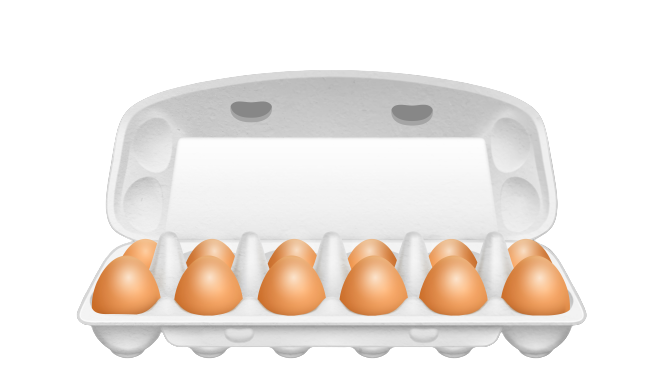
\includegraphics[width=.5\textwidth]{./media/image16a.png}
\end{figure}
\reduline{(15 x 252) : 12 = 315.\hfill}
%\reduline{É sempre recomendado escrever a expressão formada pela interpretação do enunciado, pois assim os alunos vão aprendendo a transformar textos em linguagem matemática.\hfill}

\num{10} A mãe de Beatriz comprou uma caixa de bombons para presentear os quatro filhos. 
Na caixa, os bombons estavam distribuídos em 8 fileiras de 9 unidades. 

\begin{figure}[htpb!]
\centering
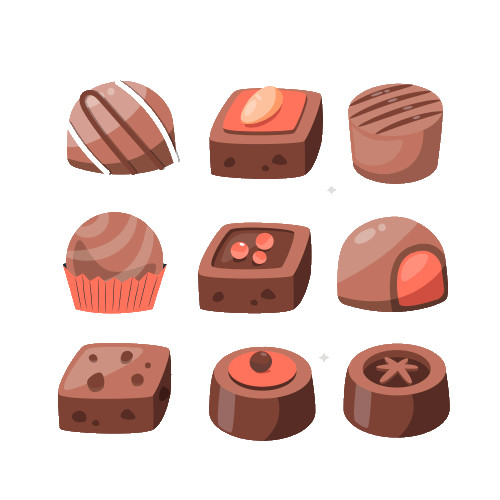
\includegraphics[width=.4\textwidth]{./media/image16b.jpeg}
\end{figure}

Calcule a quantidade de bombons que cada filho deve receber, caso todos ganhem a mesma quantidade.
\reduline{Beatriz receberá 18 bombons, assim como seus irmãos: (8 x 9) : 4 = 18.\hfill}
\linhas{1}


\num{11} Brenda se deparou com uma divisão em sua prova de matemática. 
Nela, o número 5.192 era o dividendo, e o número 22 era o divisor. 
Calcule o quociente, sabendo que Brenda acertou o cálculo.

\begin{figure}[htpb!]
\centering
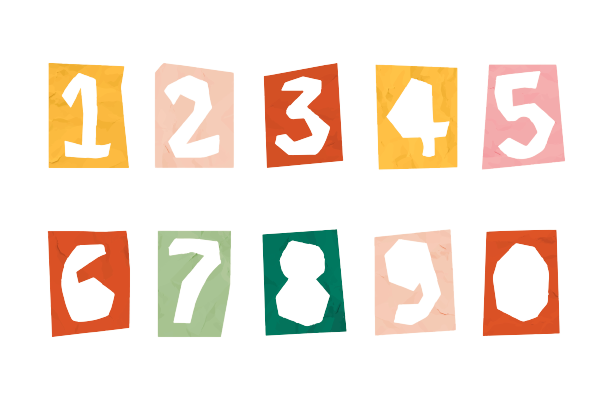
\includegraphics[width=.7\textwidth]{./media/image16c.png}
\end{figure}
%\coment{Explore também divisões com dividendos maiores.}
\reduline{5.192 : 22 = 236.\hfill}
\linhas{2}

\begin{comment}
\num{12} Observe a conversa entre Rebeca, Raquel e Renata no sítio do avô de Rebeca.

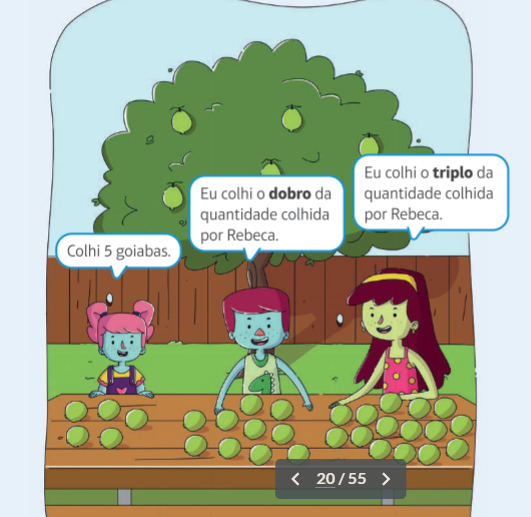
\includegraphics[width=4.42538in,height=4.30871in]{./media/image24.png}

%Fazer uma ilustração nos moldes dessa, colocando o nome de cada menina na lateral da mesa a frente delas. Na fala de Renata trocar Rebeca por Raquel. Trocar goiabas por maçãs no texto e nas frutas em cima da mesa. Trocar a palavra dobro na historinha por triplo e aumentar o número de frutas da mesa para 15 na frente dessa menina. Trocar a quantidade frutas na frente da terceira menina para 45.

\begin{escolha}
\item Qual a quantidade de maçãs que Rebeca colheu?
\reduline{5\hfill}
\linhas{2}

\item Calcule a quantidade de maçãs que Raquel colheu?
\reduline{3 x 5 = 15\hfill}
\linhas{2}

\item Qual a quantidade de maçãs que Renata colheu?
\reduline{3 x 15 = 45\hfill}
\linhas{2}
%Note. Conferir se a imagem final corresponde ao enunciado.
\end{escolha}
\end{comment}

\num{12} Complete cada frase com a palavra ``dobro'' ou com a palavra ``triplo''.

\begin{escolha}
\item
  O \reduline{dobro\hfill} de 10 é 20.
\item
  O \reduline{triplo\hfill} de 6 é 18.
\item
  O \reduline{dobro\hfill} de 7 é 14.
\item
  O \reduline{triplo\hfill} de 8 é 24.
\end{escolha}

\begin{comment}
\num{14} No quadro branco da professora Adriana, foram escritos os números a seguir:

%Construir uma figura conforme a abaixo. Os números importam e devem ser os mesmos.

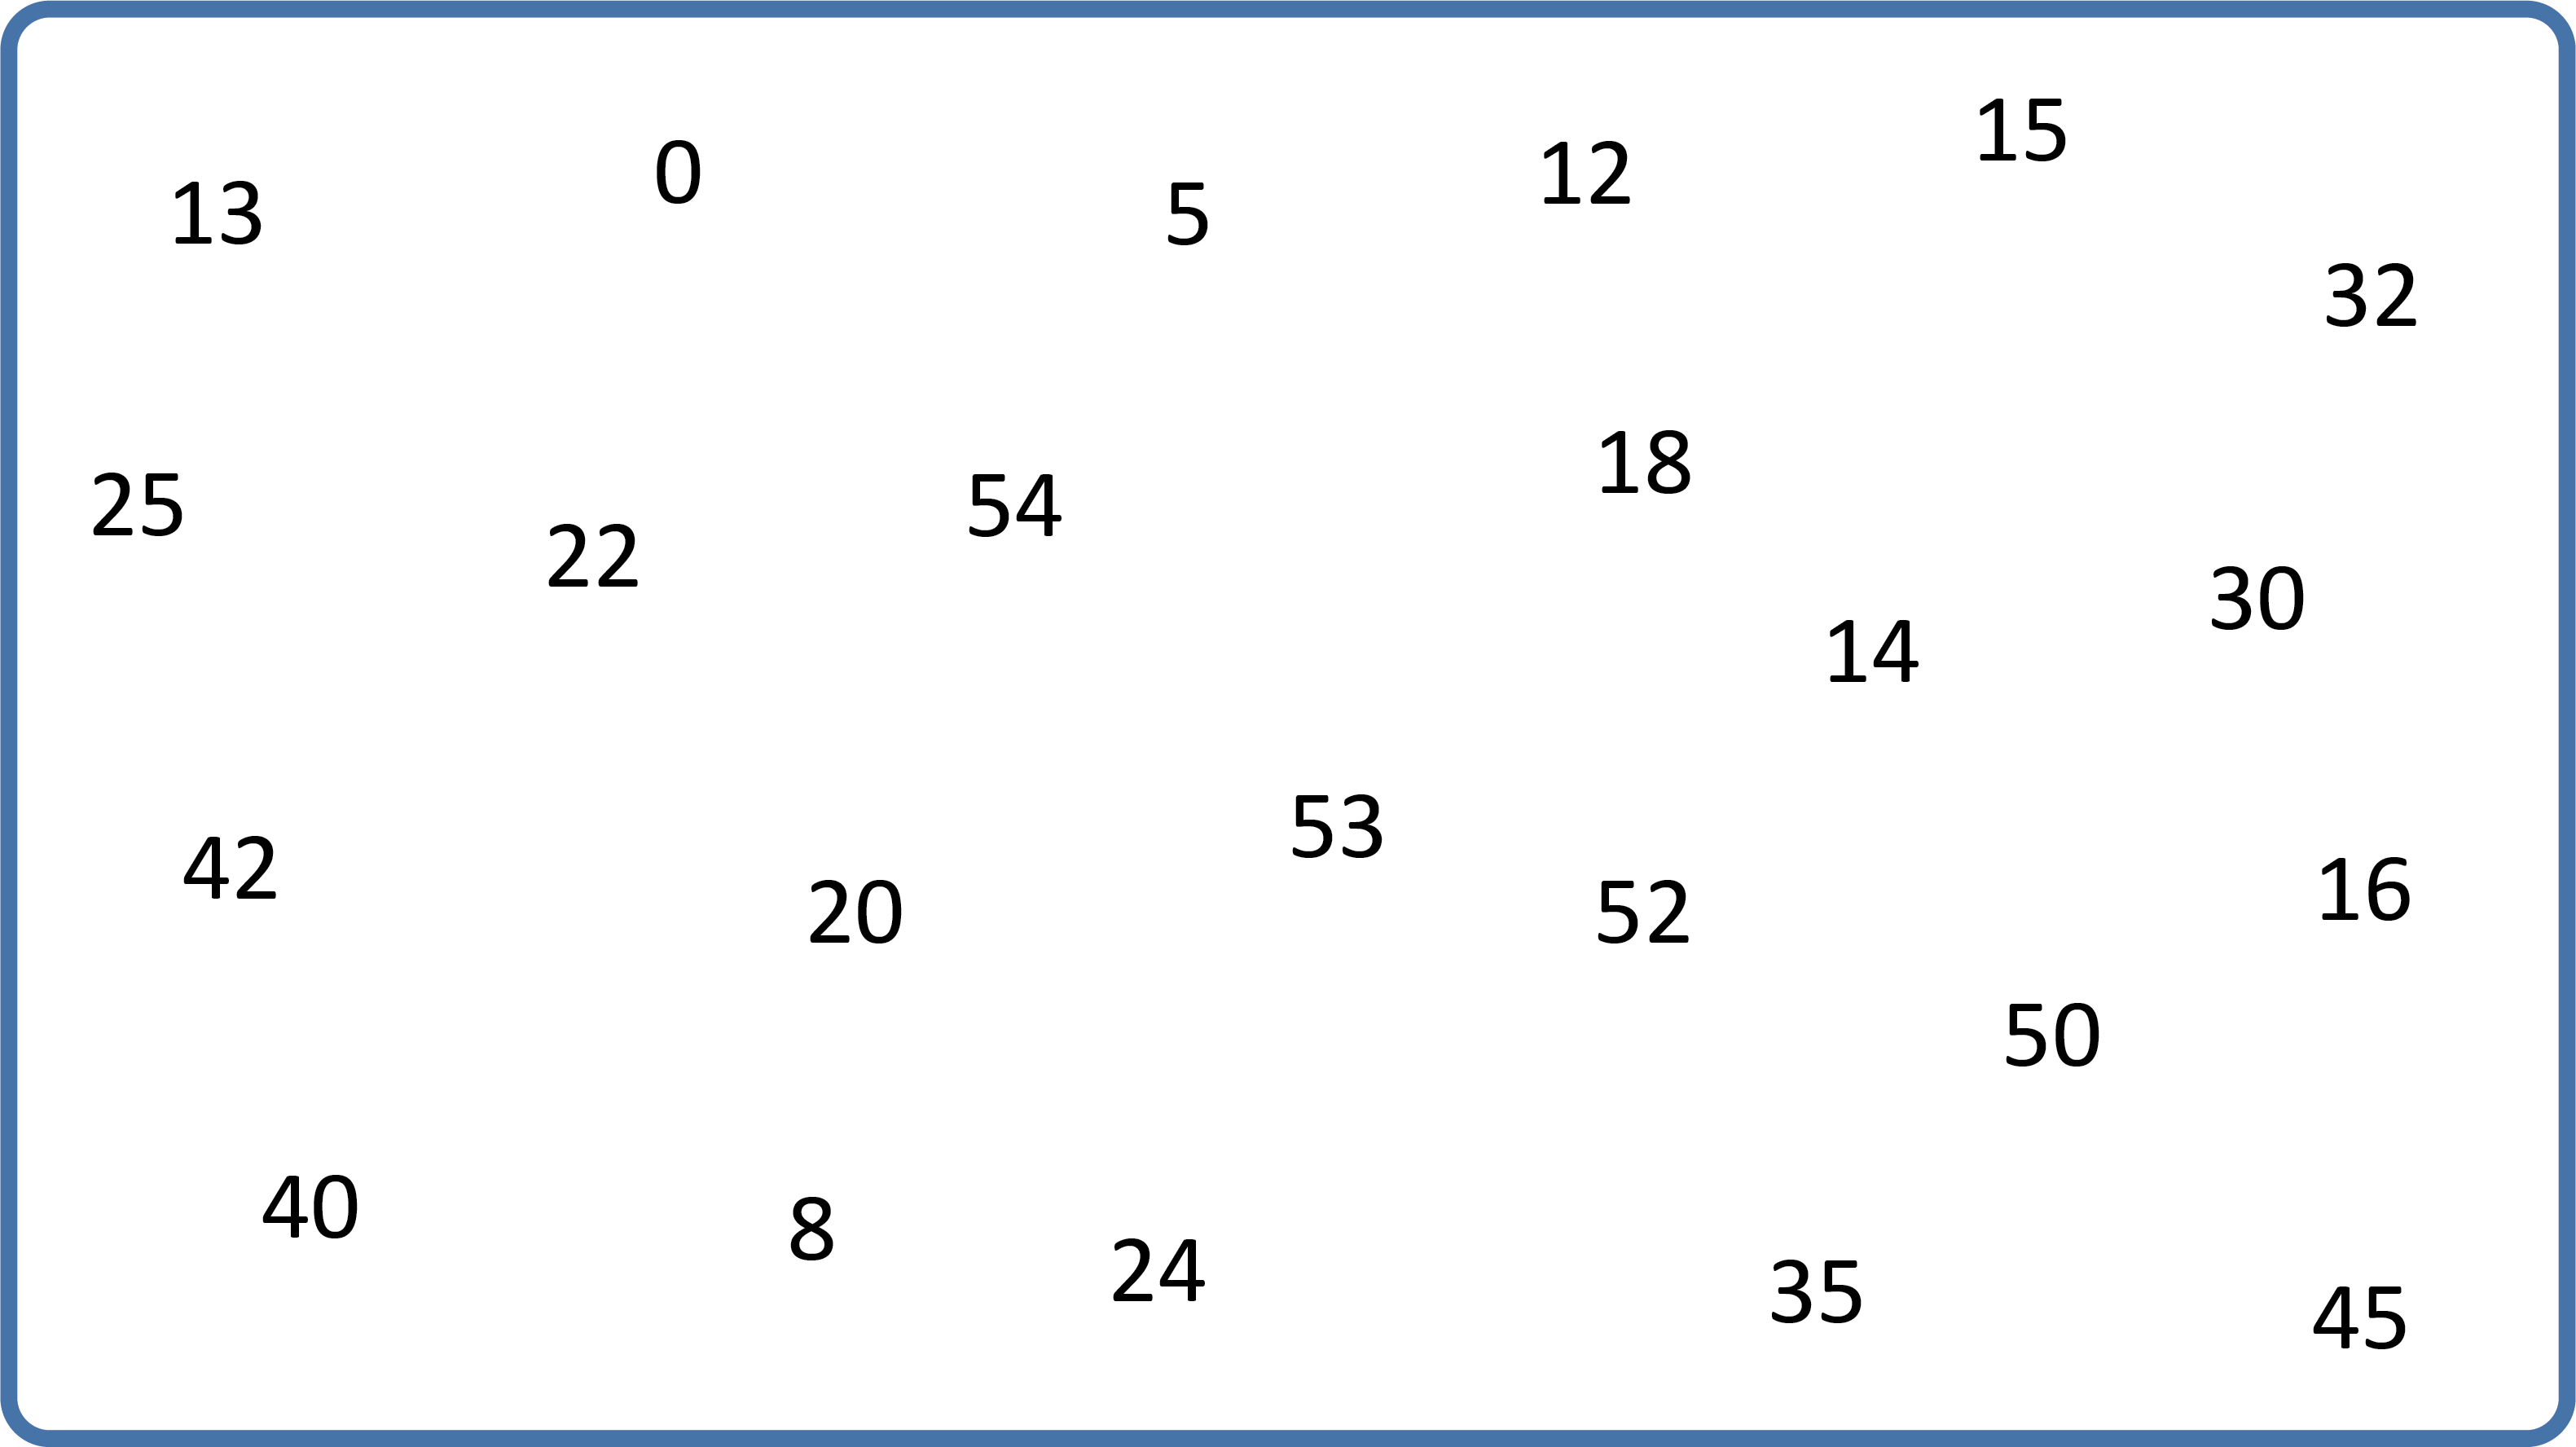
\includegraphics[width=4.51706in,height=2.09185in]{./media/image25.png}

Circule aqueles que fazem parte da tabuada do 3.

%Note. ICO. Conferir se imagem final corresponde ao texto da resposta da atidade.
\coment{12; 15; 54; 42; 24; 45.}
\end{comment}

\pagebreak

\section*{Treino}

\num{1} Uma costureira recebeu uma encomenda para colocar 6 botões em
cada uma das 9 camisas que José utiliza para trabalhar. Quantos botões
ela precisará no total para concluir a tarefa?

\begin{figure}[htpb!]
\centering
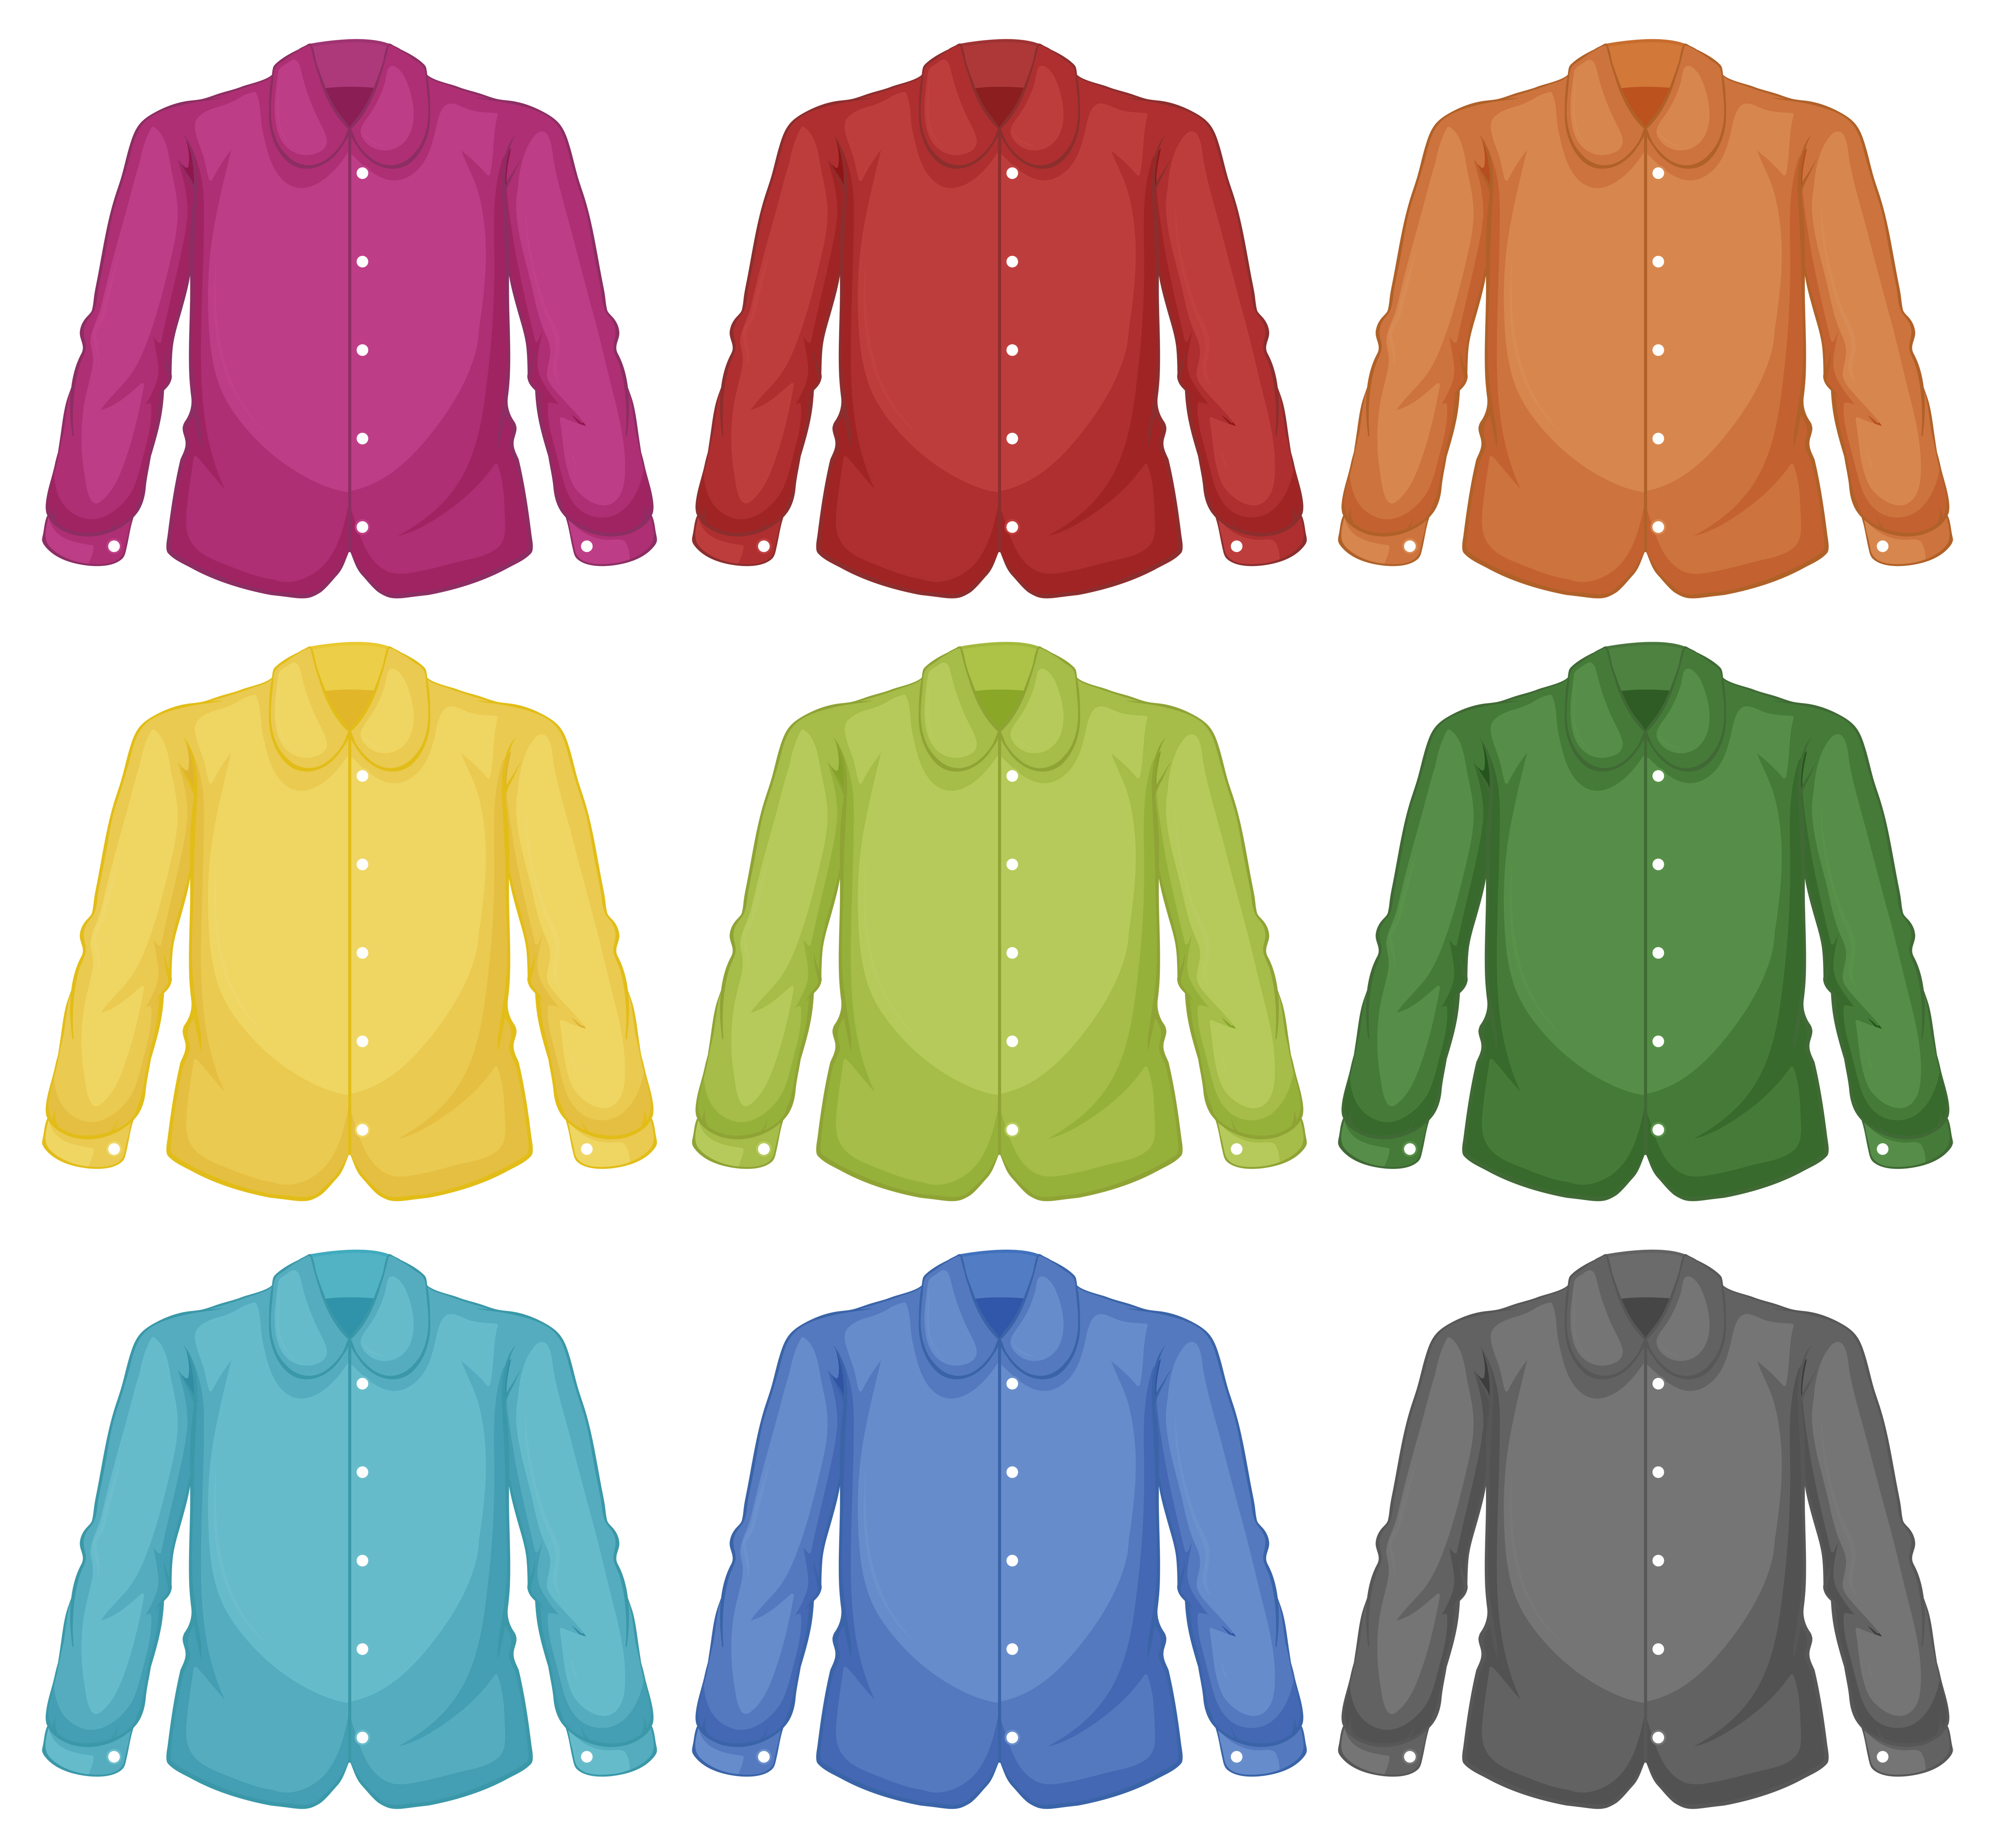
\includegraphics[width=.8\textwidth]{./media/image16d.jpeg}
\end{figure}

\begin{escolha}
    \item 6.
    \item 9.
    \item 15.
    \item 54.
\end{escolha}

\pagebreak

\num{2} Para uma festa familiar, a mãe de Josué comprou 12 fardos de
suco como os representados pela imagem a seguir. Quantas garrafas de suco foram compradas para a festa? 
%Incluir imagem disponível em https://br.freepik.com/vetores-gratis/latas-em-embalagens-plasticas_11684670.htm#query=six%20pack%20soda&position=0&from_view=search&track=robertav1_2_sidr

\begin{minipage}{.5\textwidth}
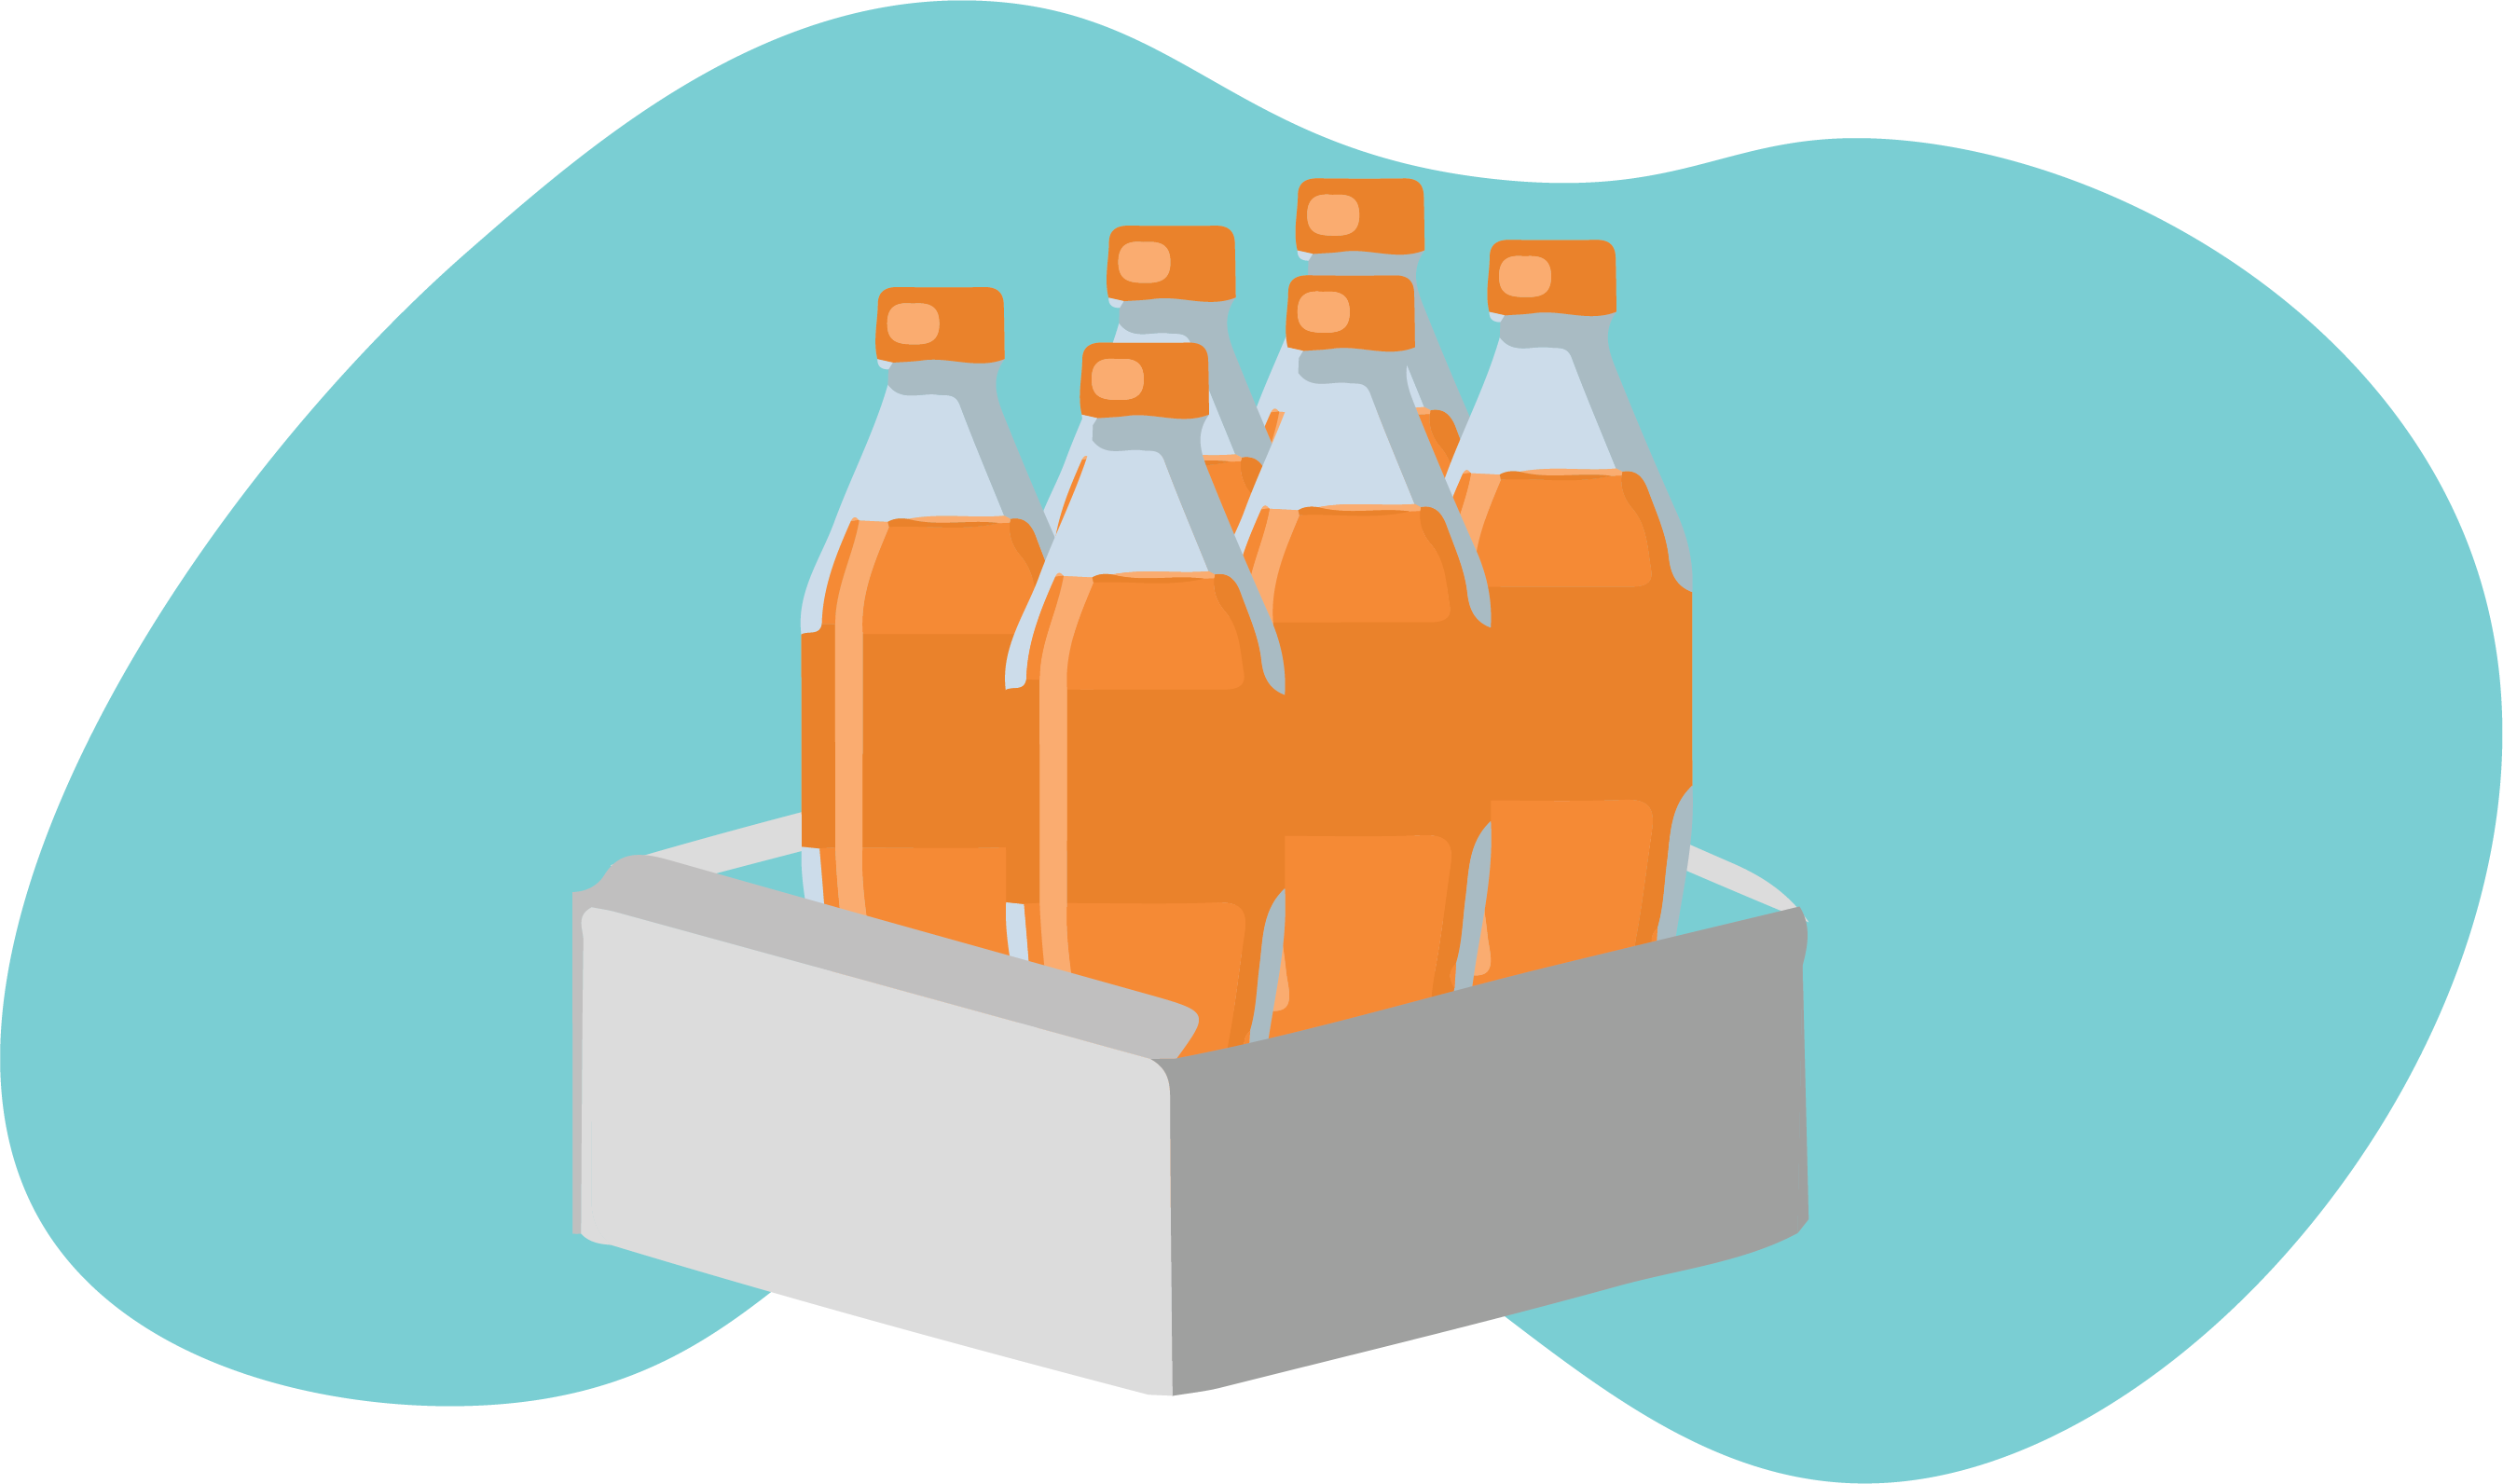
\includegraphics[width=\textwidth]{./media/image26.png}
\end{minipage}
\begin{minipage}{.5\textwidth}
\begin{escolha}
\item
  6 garrafas de suco.
\item
  12 garrafas de suco.
\item
  72 garrafas de suco.
\item
  144 garrafas de suco.
\end{escolha}
\end{minipage}

\num{3} Um campeonato interno de basquete será promovido na escola em que Carlos
estuda. Pelas regras, cada time deverá ter 5 jogadores titulares e mais 3 reservas. Considerando que serão formados 6 times, qual é a quantidade de alunos que poderão participar do campeonato?

\begin{figure}[htpb!]
\centering
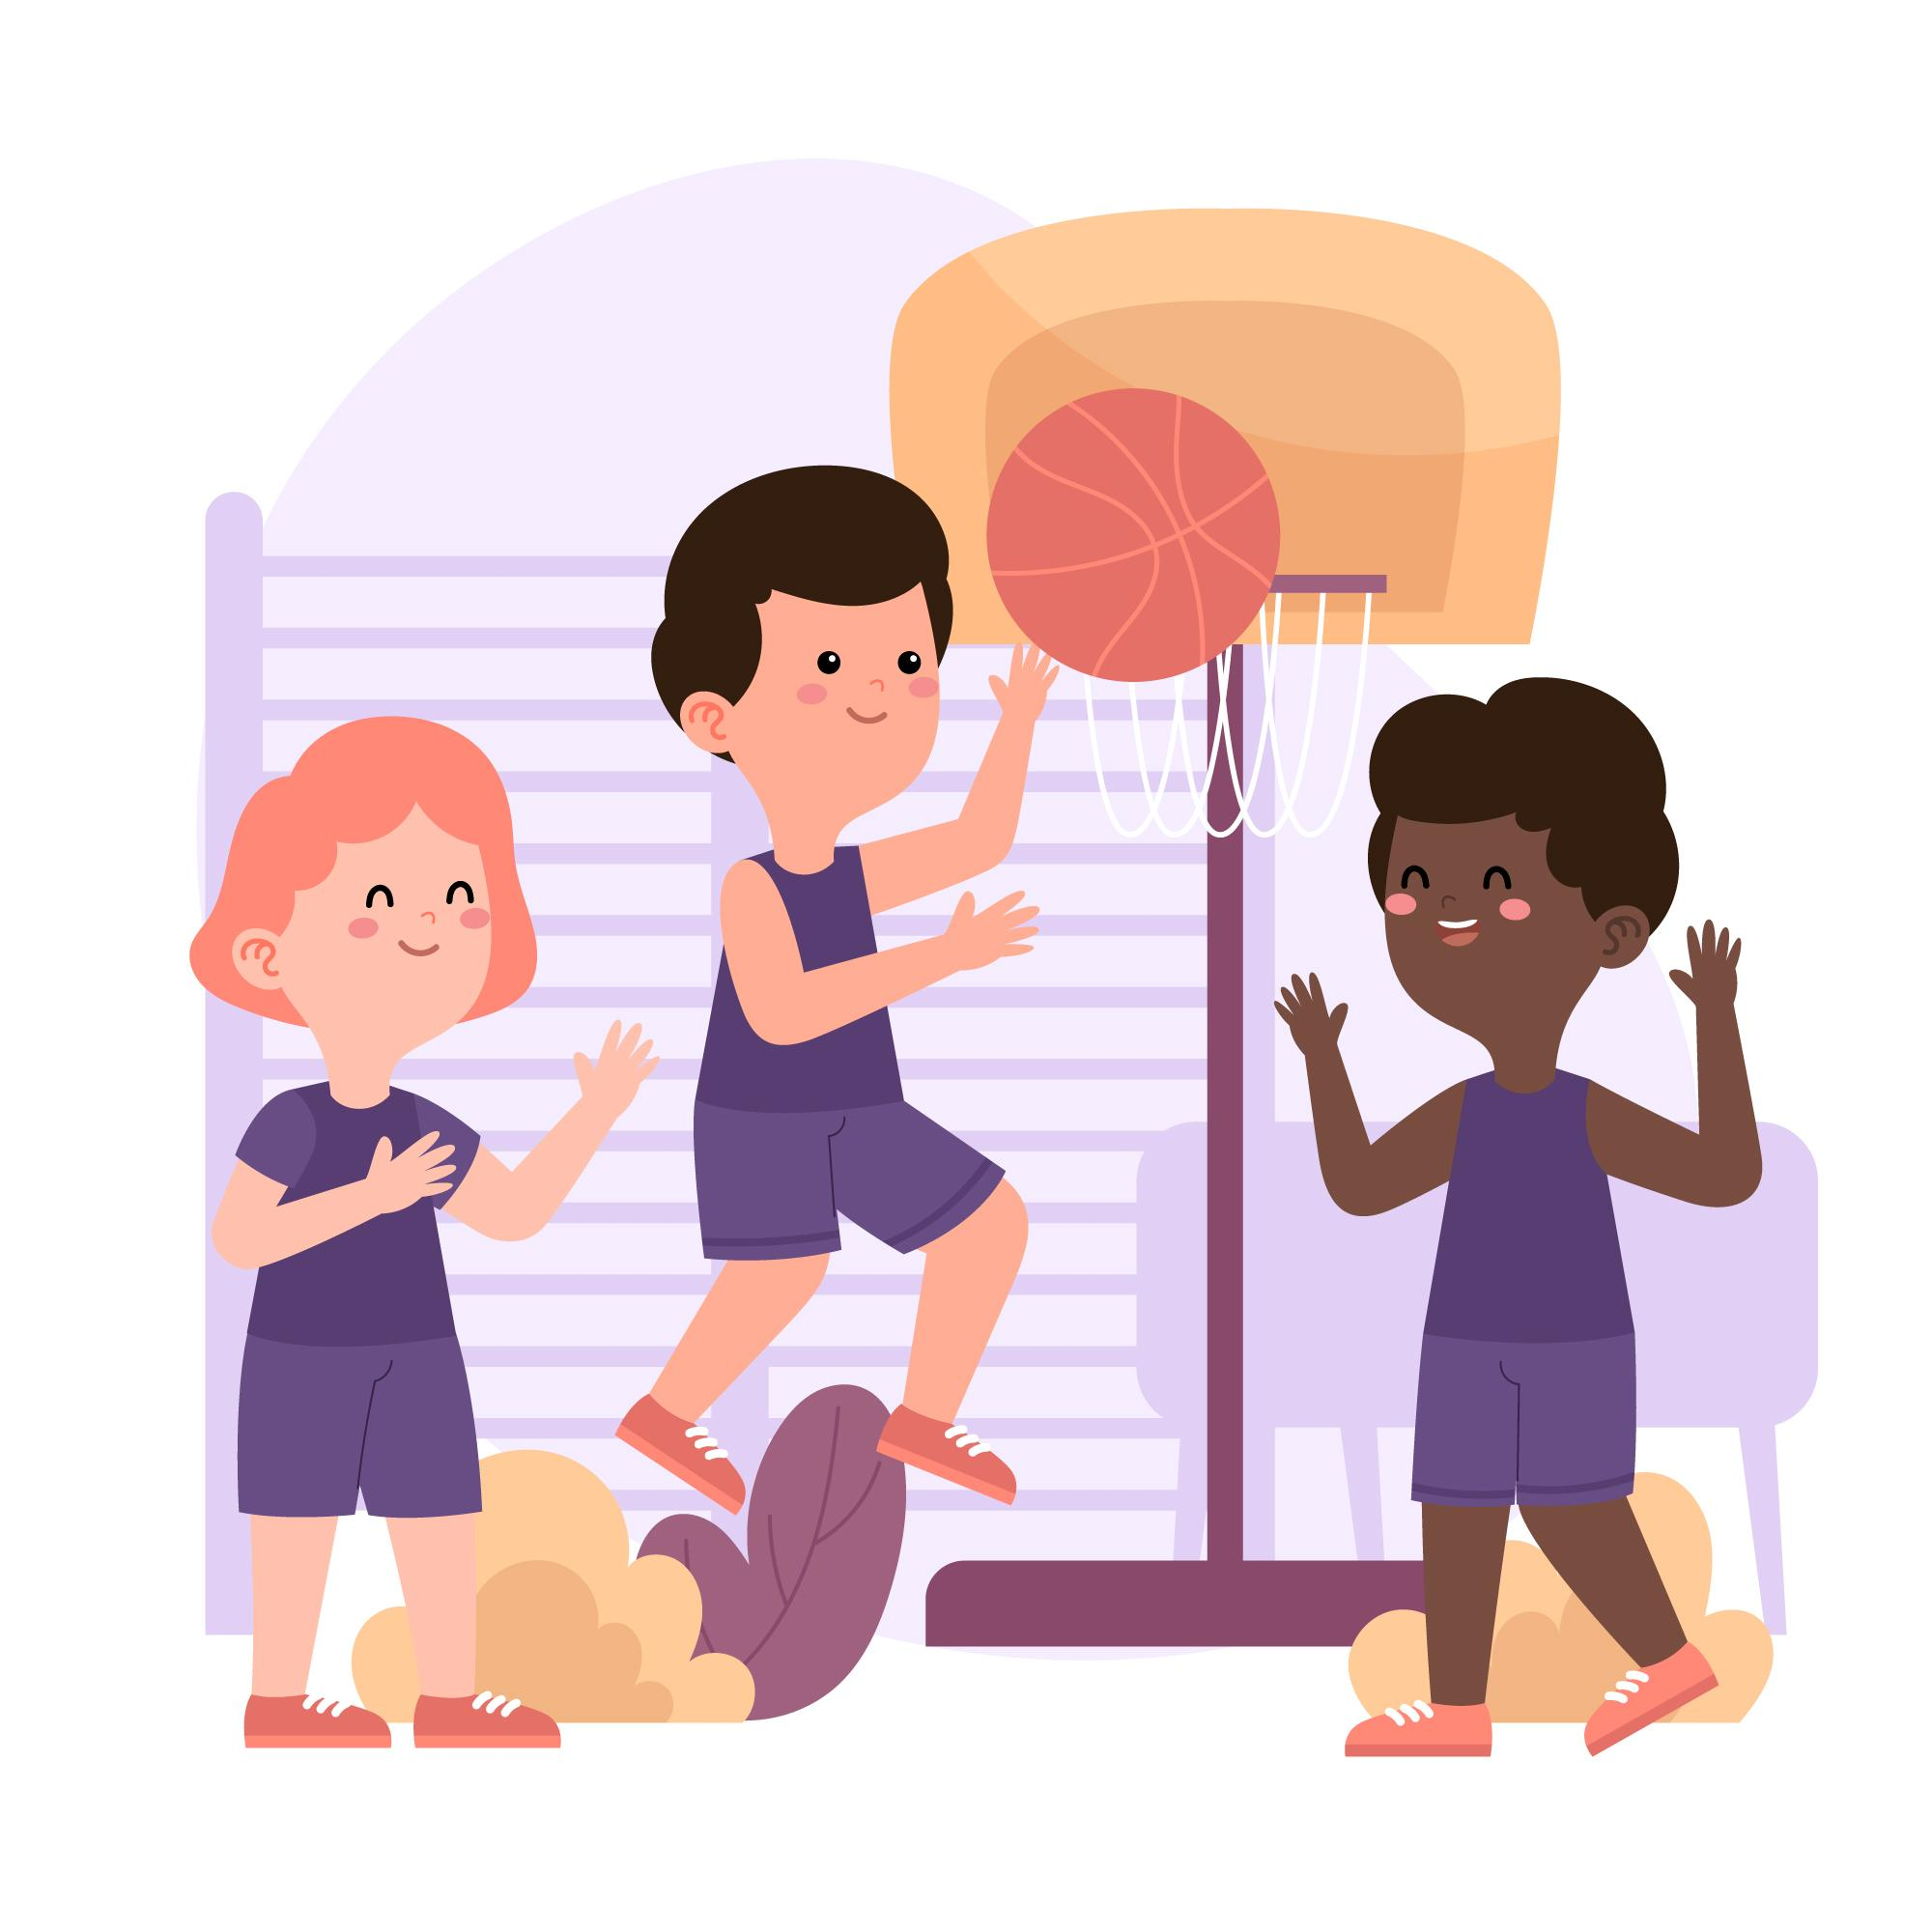
\includegraphics[width=.6\textwidth]{./media/image16e.jpeg}
\end{figure}

\begin{multicols}{2}
\begin{escolha}
\item
  18.
\item
  30.
\item
  36.
\item
  48.
\end{escolha}
\end{multicols}
\chapter{Descobertas e sequências}
\markboth{Módulo 3}{}\enlargethispage{\baselineskip}

\section*{Habilidades do SAEB}

\begin{itemize}
\item Inferir ou descrever atributos ou propriedades comuns que os elementos
que constituem uma sequência recursiva de números naturais apresentam.

\item Inferir o padrão ou a regularidade de uma sequência de números
naturais ordenados, objetos ou figuras.

\item Inferir os elementos ausentes em uma sequência de números naturais
ordenados, objetos ou figuras.
\end{itemize}

\subsection{Habilidade da BNCC}

\begin{itemize}
\item EF03MA10.
\end{itemize}

\conteudo{
\begin{center}
\textbf{Sequências}
\end{center}

Uma sequência ou sucessão é um conjunto numérico ordenado, no qual existe sempre uma lógica de formação.

Na sequência numérica dos números naturais, com exceção do zero, todos os termos possuem um antecessor. O antecessor é o número imediatamente anterior na sequência. 

Na sequência numérica dos números naturais, todos os termos possuem um sucessor. O sucessor de um número é aquele imediatamente posterior na sequência. 

Exemplos de sequências

\begin{itemize}
\item 
  A escalação de um time de futebol de salão pode ser ordenada pela primeira letra dos nomes dos jogadores, ou seja, em ordem alfabética:
\end{itemize}

\begin{myquote}
\centering
\textbf{Alan, Bruno, Fernando, Igor, Tácio.}
\end{myquote}

\begin{itemize}
\item 
  Uma sequência pode ser formada pelos números pares:
\end{itemize}

\begin{myquote}
\centering
\textbf{0; 2; 4; 6; 8; 10; 12; ...}
\end{myquote}

As sequências podem ser classificadas quanto ao número de elementos que apresentam ou podem apresentar.

\begin{itemize}
\item
  Sequência finita apresenta número definido de termos,
  ou seja, 10 termos, 20 termos, 8 termos.
\item
  Sequência infinita apresenta número infinito de termos, como a sequência dos números naturais.
\end{itemize}

Ainda podemos classificar as sequências em:

\begin{itemize}
\item
  Sequência crescente: aquela em que cada termo sucessor é maior que seu antecessor.
\end{itemize}

\begin{myquote}
\centering
\textbf{Exemplo: 5, 10, 15, 20, 25.}
\end{myquote}

\begin{itemize}
\item
  Sequência decrescente: aquela em que cada termo sucessor sempre é menor do que seu antecessor.
\end{itemize}

\begin{myquote}
\centering
\textbf{Exemplo: 9, 7, 5, 3.}
\end{myquote}
}

\section*{Atividades}

\num{1} A professora Mariana colocou seus alunos posicionados em uma fila, 
%iniciada pelo aluno de tênis azul e mochila alaranjada, 
como na imagem a seguir.

\begin{figure}[htpb!]
\centering
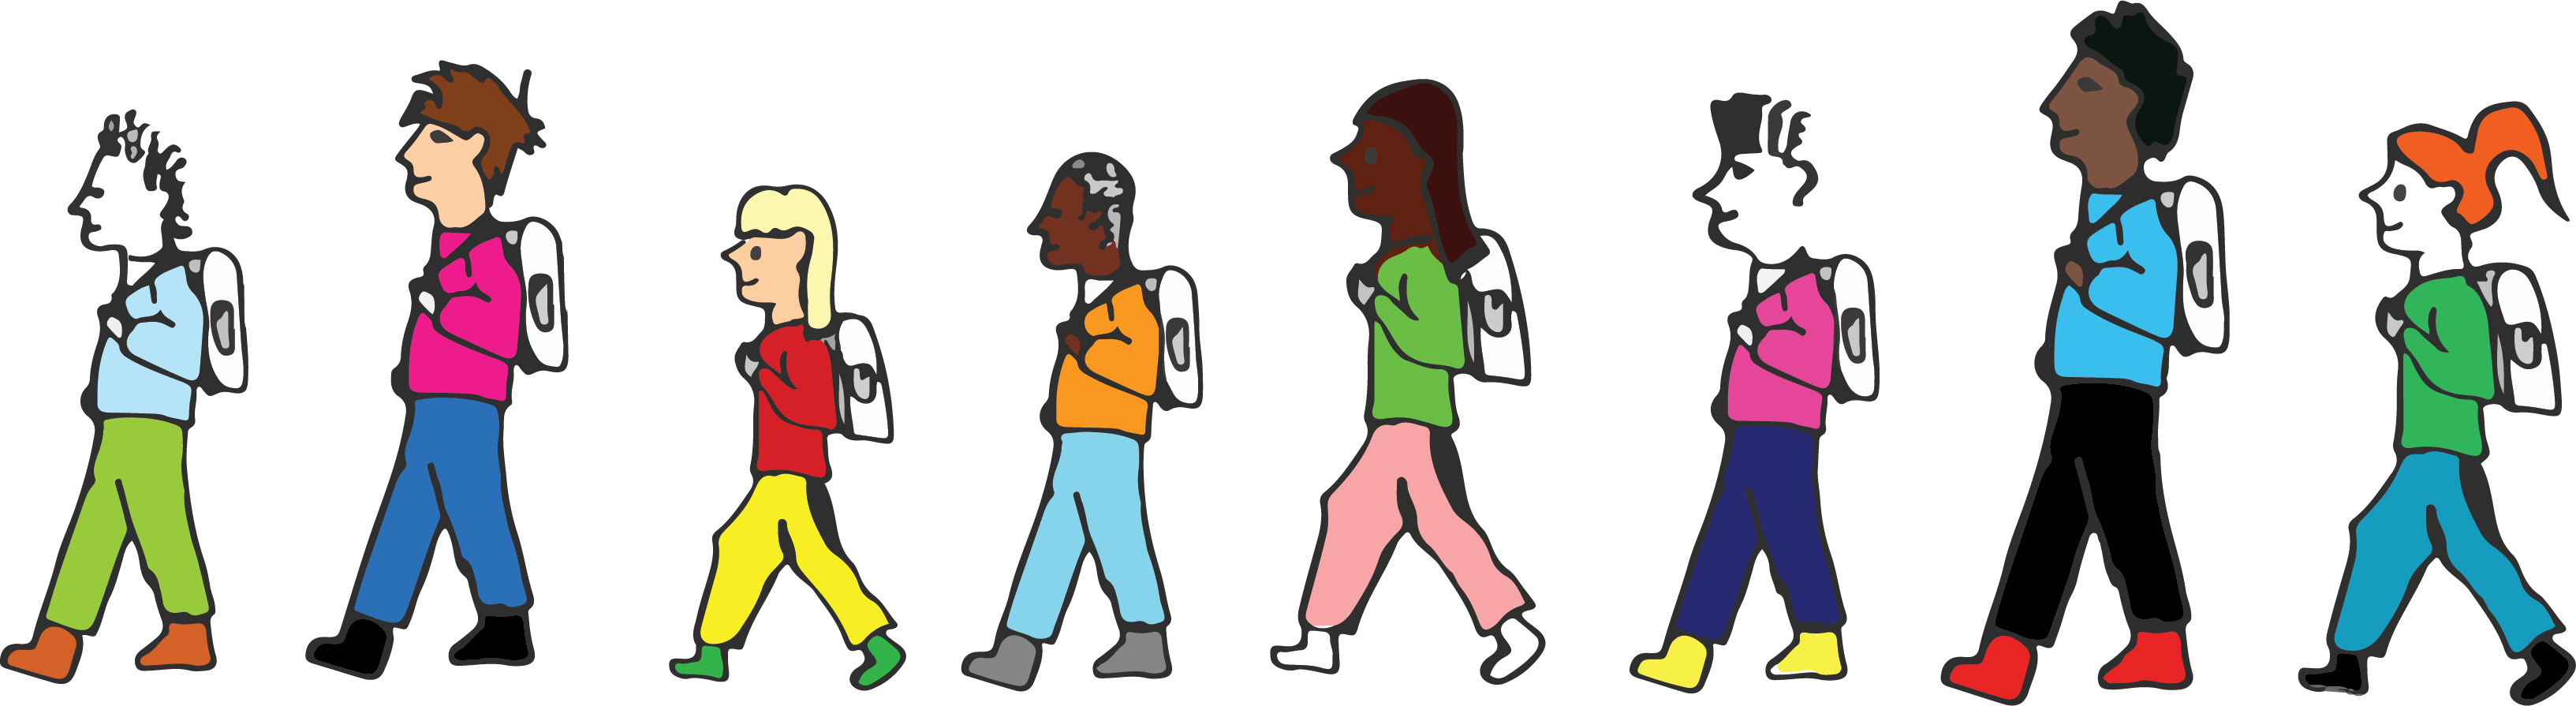
\includegraphics[width=\textwidth]{./media/image27.png}
\end{figure}

Observe atentamente a figura e responda ao que se pede.

\begin{escolha}
\item Qual a posição da criança mais baixa na fila? 
\reduline{A criança mais baixa está na 3º posição (terceira posição) na fila.\hfill}

\item Qual a posição da criança mais alta na fila? 
\reduline{A criança mais alta está na 7º posição (sétima posição) na fila.\hfill}
\end{escolha}

\num{2} O pai de Marcelo mostrou a ele uma sequência de bolinhas pintadas com
diversas cores.

\begin{figure}[htpb!]
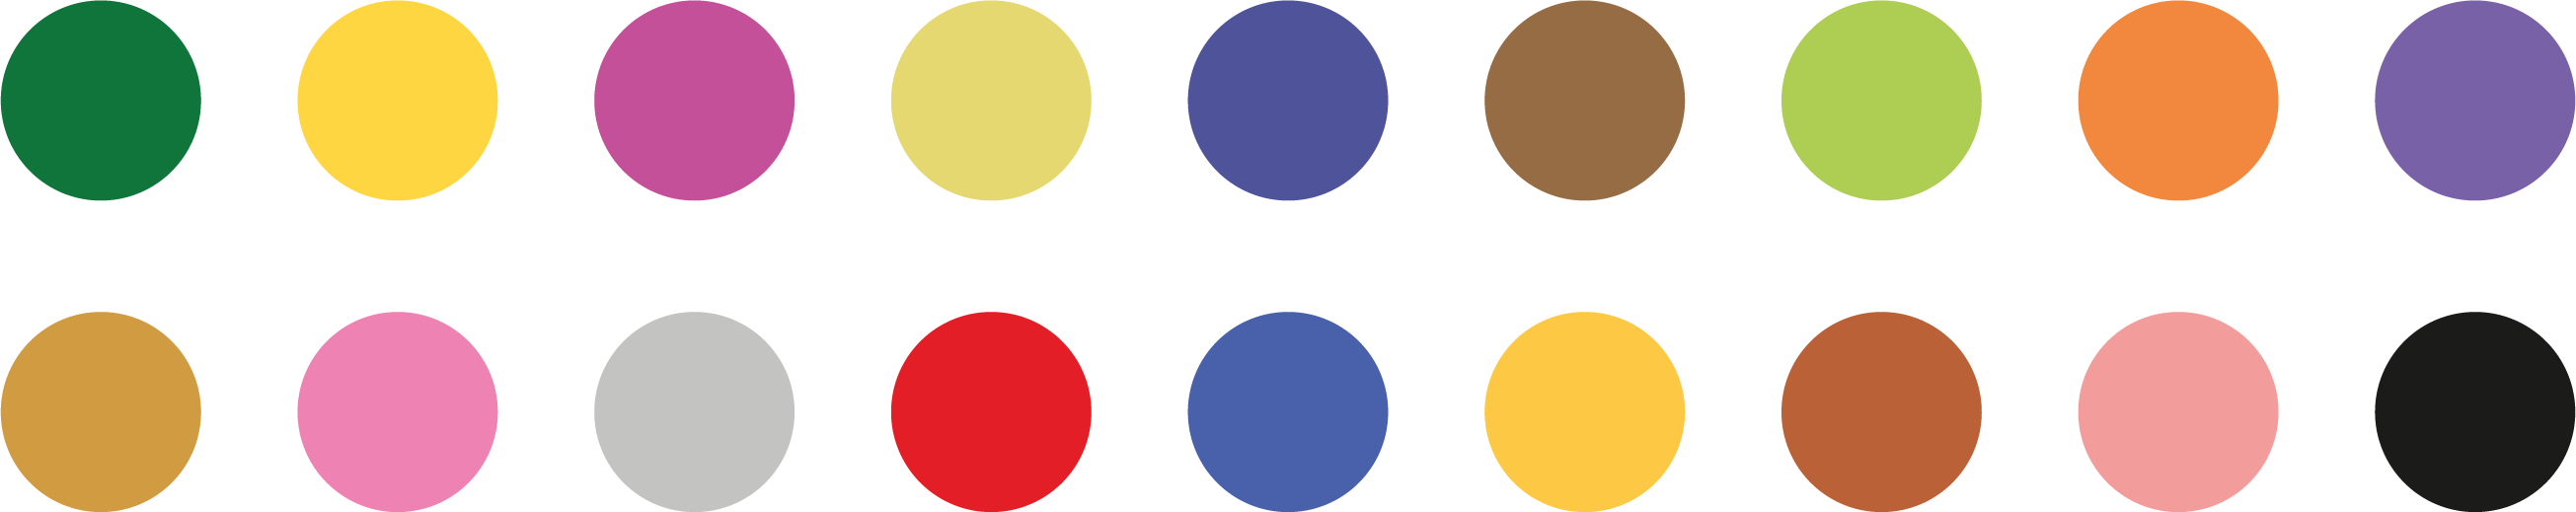
\includegraphics[width=\textwidth]{./media/image28.png}
\end{figure}

Observando essa sequência percebemos que a bolinha pintada com a cor
verde-escuro é a primeira, e a bolinha pintada com a cor preta é a
última.

Quais as posições das bolinhas pintadas com a cor azul?
\reduline{As bolinhas pintadas com a cor azul estão na 5º (quinta) posição e na
14º (décima quarta) posição.\hfill}


\num{3} Na prova de matemática que Manoela acabou de fazer estava o seguinte exercício:

\begin{myquote}
Escreva uma sequência de números de forma crescente, de 10 em 10, começando no número 705 até o sétimo termo.

%\begin{figure}[htpb!]
%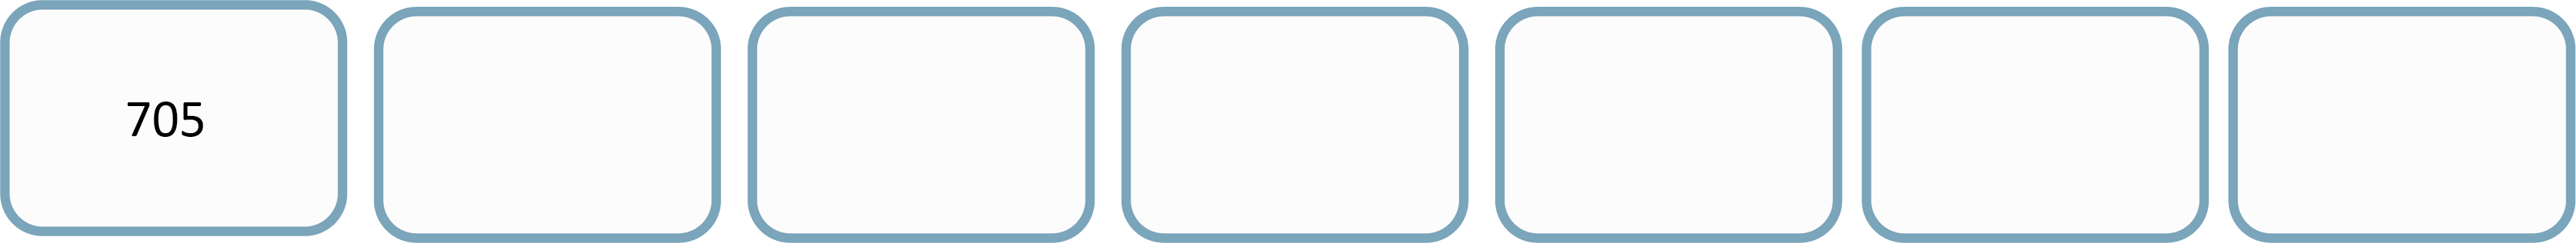
\includegraphics[width=\textwidth]{./media/image29.png}
%\end{figure}

\end{myquote}

Resolva a atividade proposta na prova de Manuela.
\reduline{705; 715; 725; 735; 745; 755; 765.\hfill}
\linhas{2}


\num{4} Rafaela foi a uma loja de brinquedos e, para ser atendida, pegou a senha de
número 32. Todos são atendidos pela ordem numérica das senhas.


%incluir imagem disponível em https://br.freepik.com/fotos-gratis/mulher-sorridente-segurando-o-cartao-de-visita-em-branco_24488868.htm#query=senha\%20de\%20atendimento\&position=41\&from_view=search\&track=robertav1_2_sidr

\begin{escolha}
\item Qual é o número da pessoa que foi atendida imediatamente antes de Rafaela?
\reduline{O número 31, pois é o antecessor de 32.\hfill}

\item Qual é o número da pessoa que será atendida imediatamente depois de Rafaela?
\reduline{O número 33, pois é o sucessor de 32.\hfill}
\end{escolha}

\pagebreak

\num{5} Alice organizou os nomes dos amigos que pretende convidar para sua
festa de aniversário em uma lista numerada.

\begin{figure}[htpb!]
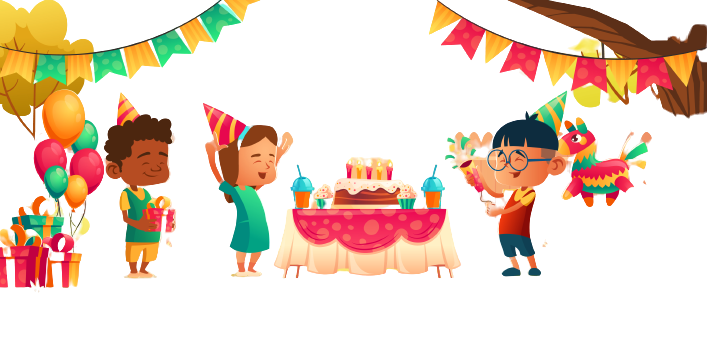
\includegraphics[width=\textwidth]{./media/image28a.png}
\end{figure}

\begin{myquote}
\begin{enumerate}
\begin{multicols}{2}
\item Ana

\item Ana Clara

\item Augusto

\item Bernardo

\item Camila

\item Daniel
\end{multicols}
\end{enumerate}
\end{myquote}

Observando a lista, responda ao que se pede.

\begin{escolha}
\item Qual o nome do amigo que aparece na posição do sucessor de 4?
\reduline{Camila, pois o sucessor do 4 é o 5.\hfill}

\item Qual o nome do amigo que aparece diante do antecessor de 3?
\reduline{Ana Clara, pois o antecessor do 3 é o 2.\hfill}

\item O número representado por Ana é antecessor de qual número?
\reduline{É antecessor de 2, já que Ana aparece no número 1.\hfill}
\end{escolha}

\pagebreak
\num{6} Observe o quadro que Roberta encontrou no caderno de seu irmão.

\begin{figure}[htpb!]
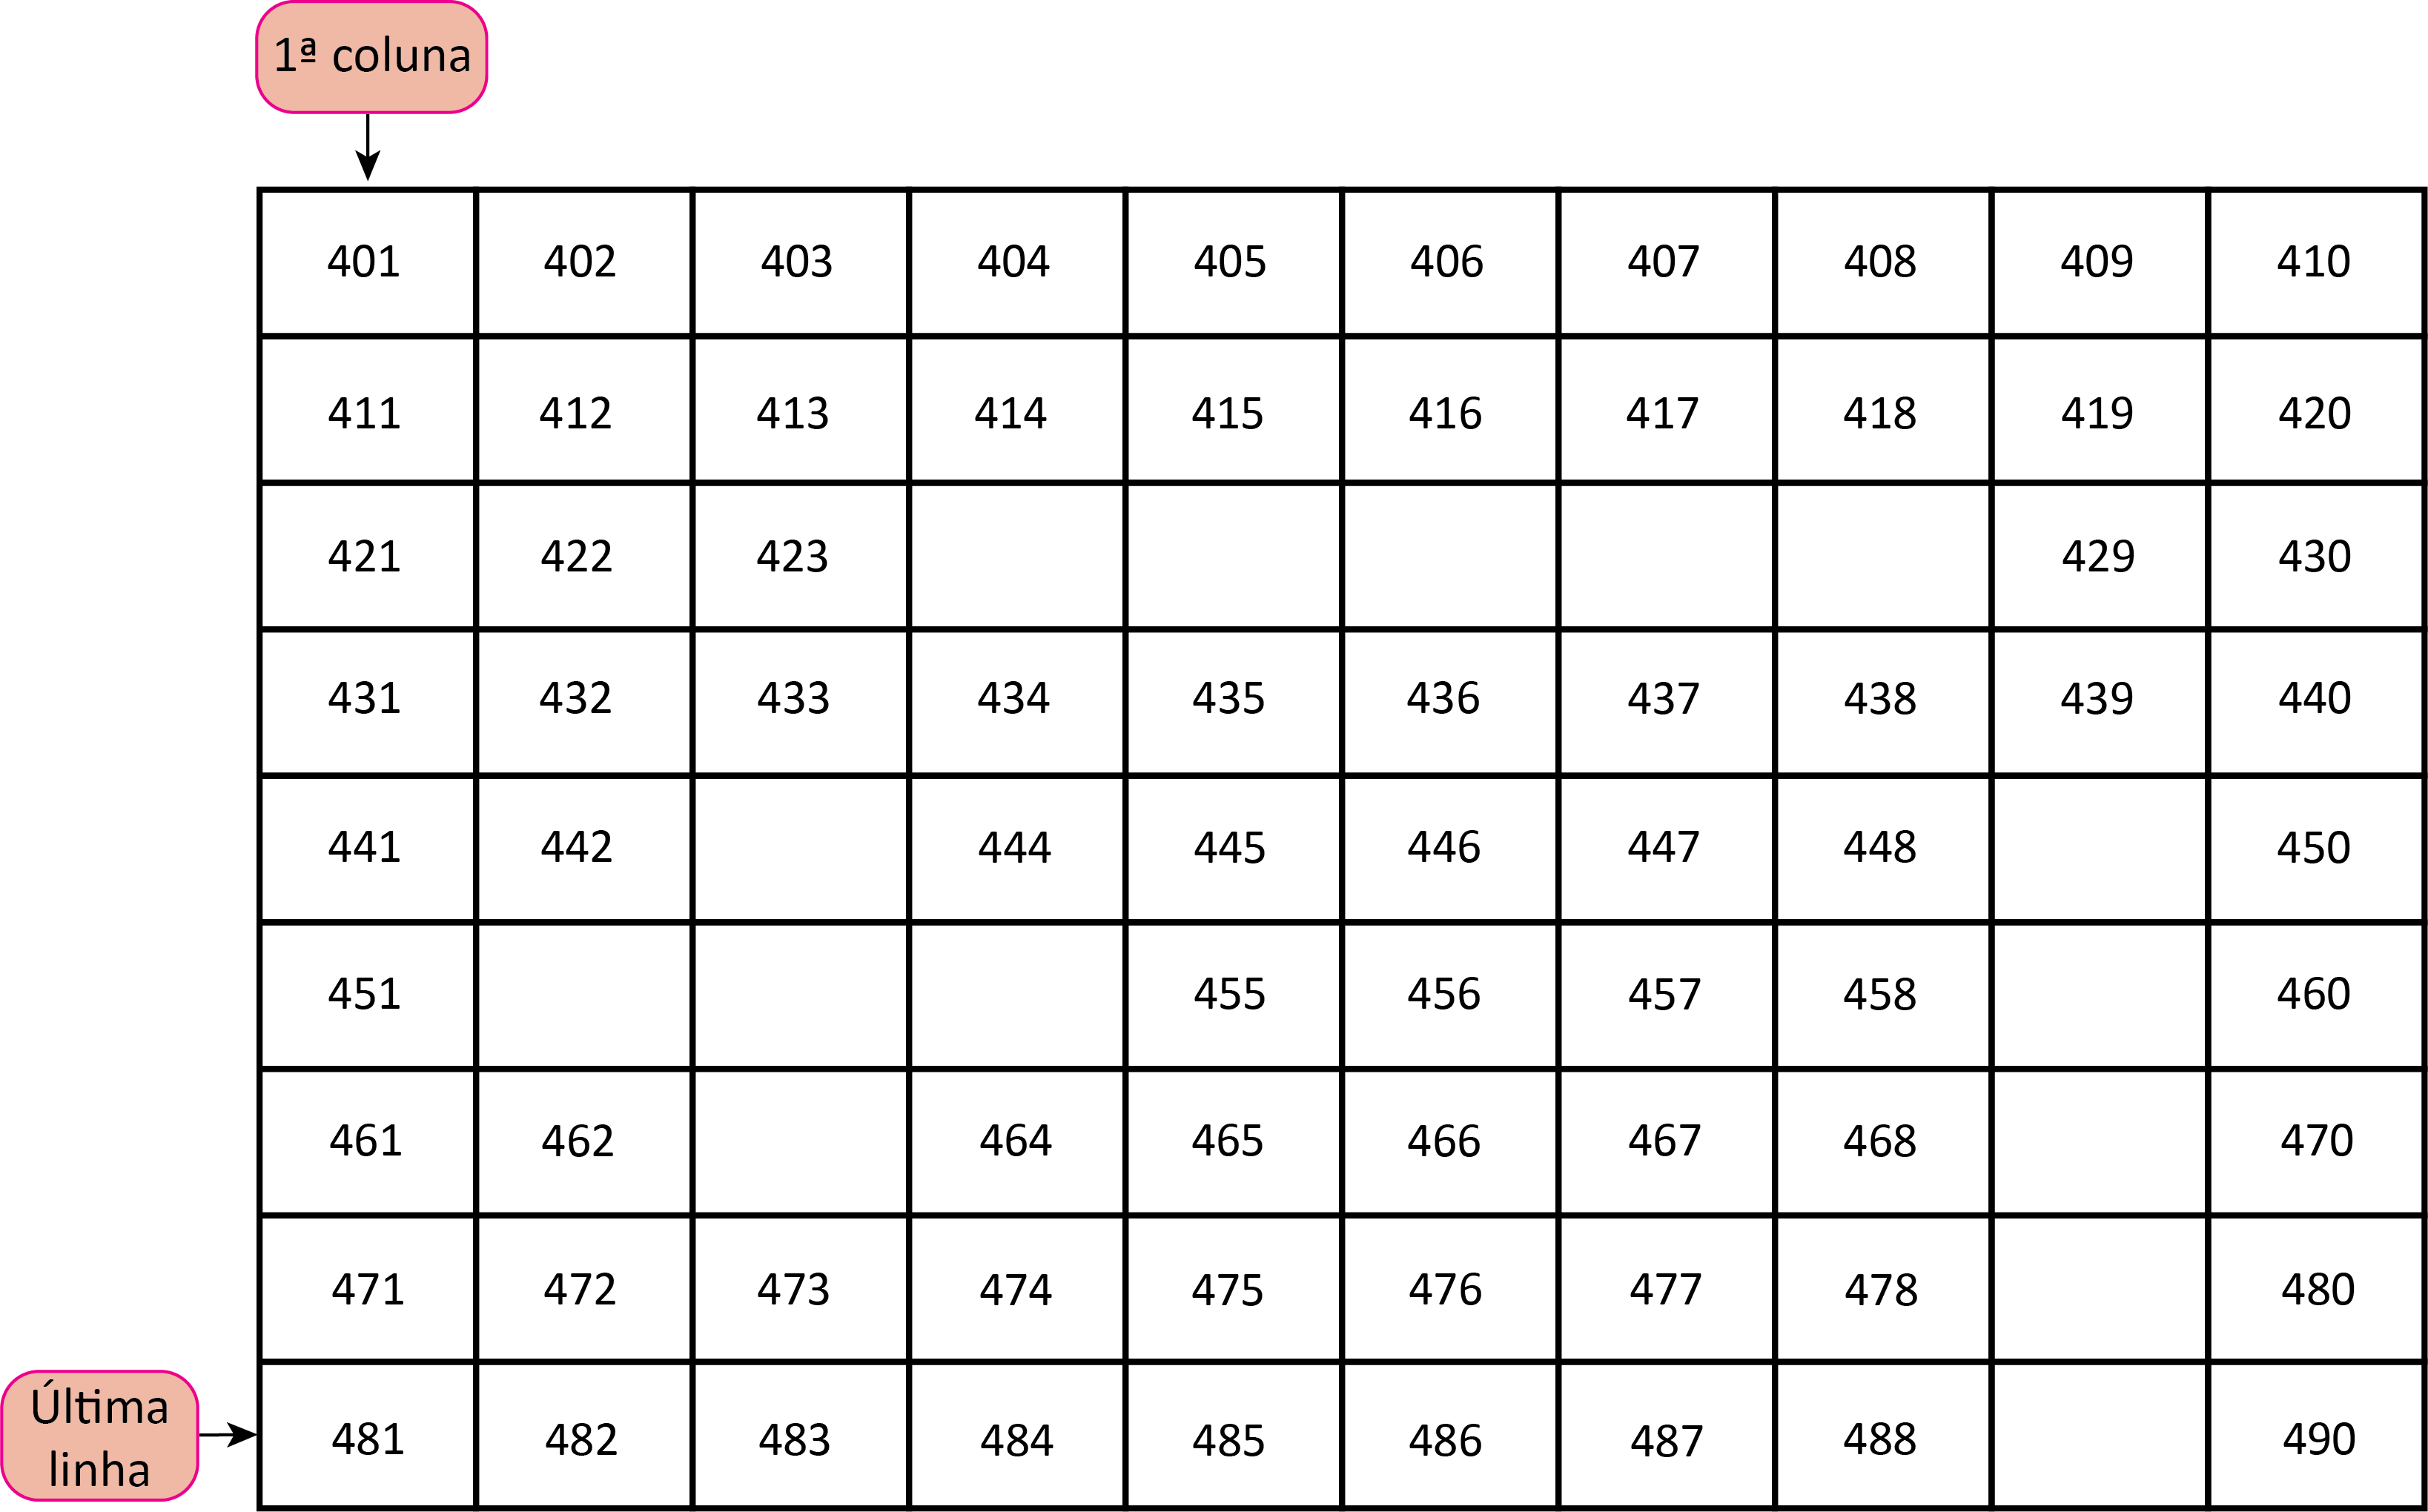
\includegraphics[width=\textwidth]{./media/image30.png}
\end{figure}

\begin{escolha}
\item Preencha os espaços vazios com os números que estão faltando.\coment{3ª linha: 424, 425, 426, 427, 428; 5ª linha: 443, 449; 6ª linha: 452, 453, 454, 459; 7ª linha: 463, 469; 8ª linha: 479; 9ª linha: 489.}

\item Qual é o número que está na 3ª coluna e na 4ª linha?
\reduline{433.\hfill}
\linhas{2}

\item Qual é a linha e a coluna em que o número quatrocentos e setenta e seis está?
\reduline{6ª coluna, 8ª linha.\hfill}
\linhas{2}
\end{escolha}

\vspace{-2ex}

\num{7} Observe a reta numérica que representa a sequência dos números naturais e responda a cada item a seguir.

\begin{figure}[htpb!]
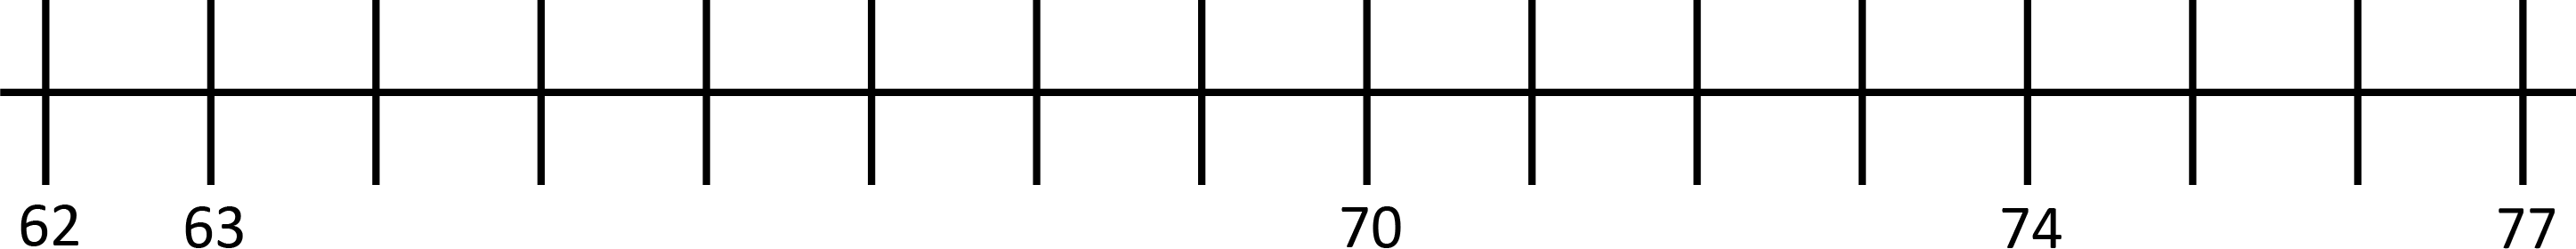
\includegraphics[width=\textwidth]{./media/image31.png}
\end{figure}

\begin{escolha}
\item Qual o número natural que será escrito imediatamente após o número 75?
\reduline{76, pois é o sucessor de 75.\hfill}

\item Qual o número natural que virá escrito antes do número 68 nessa reta numérica?
\reduline{67, pois é o antecessor de 68.\hfill}

\item Qual o antecessor do número setenta e sete?
\reduline{76.\hfill}

\item Qual o sucessor do número setenta e quatro?
\reduline{75.\hfill}
\end{escolha}

\num{8} Escreva os números naturais de cada item em ordem crescente.

\begin{escolha}
\item 30; 25; 10; 5; 20; 15
\reduline{5; 10; 15; 20; 25; 30.\hfill}

\item 7; 21; 14; 35; 28
\reduline{7; 14; 21; 28; 35.\hfill}

\item 16; 8; 12; 4; 24; 20
\reduline{4; 8; 12; 16; 20; 24.\hfill}
\end{escolha}

\num{9} Em cada item, indique se a sequência é crescente ou decrescente.

\begin{escolha}
\item 10; 8; 6; 4; 2; 0
\reduline{Decrescente.\hfill}

\item 10; 20; 30; 40; 50
\reduline{Crescente.\hfill}

\item 21; 19; 17; 15; 13
\reduline{Decrescente.\hfill}

%\item 6; 12; 18; 24; 30; 36
%\reduline{Crescente.\hfill}
\end{escolha}

\num{10} Observe as sequências dadas e determine, sem fazer desenhos, a
quantidade de bolinhas que a figura 8 de cada sequência terá.

\begin{escolha}
\item \reduline{3; 6; 9; 12; 15; 18; 21; 24; ou 3 x 8 = 24.\hfill} bolinhas

\begin{center}
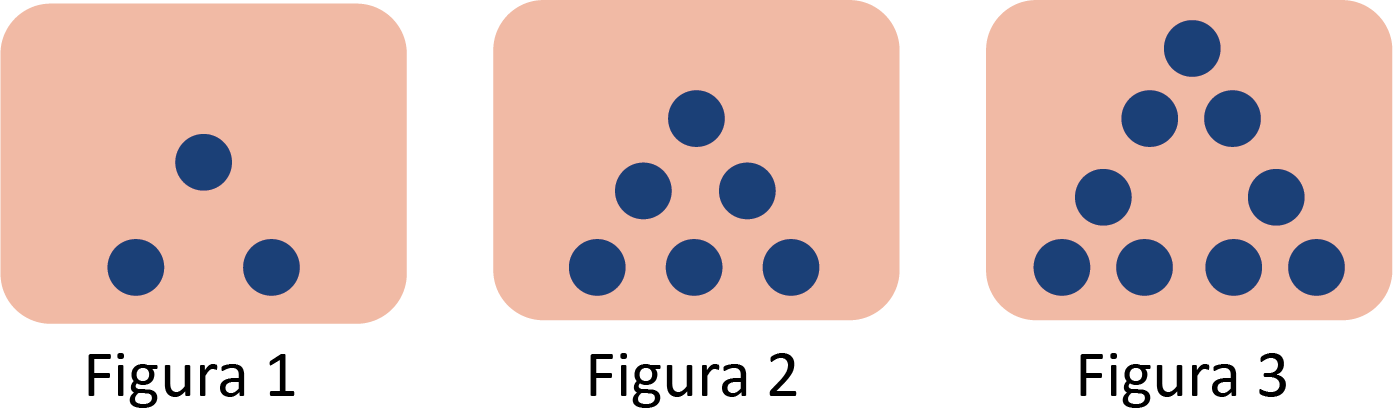
\includegraphics[width=.7\textwidth]{./media/image33.png}
\end{center}

\item \reduline{4; 8; 12; 16; 20; 24; 28; 32; ou 8 x 4 = 24.\hfill} bolinhas

\begin{center}
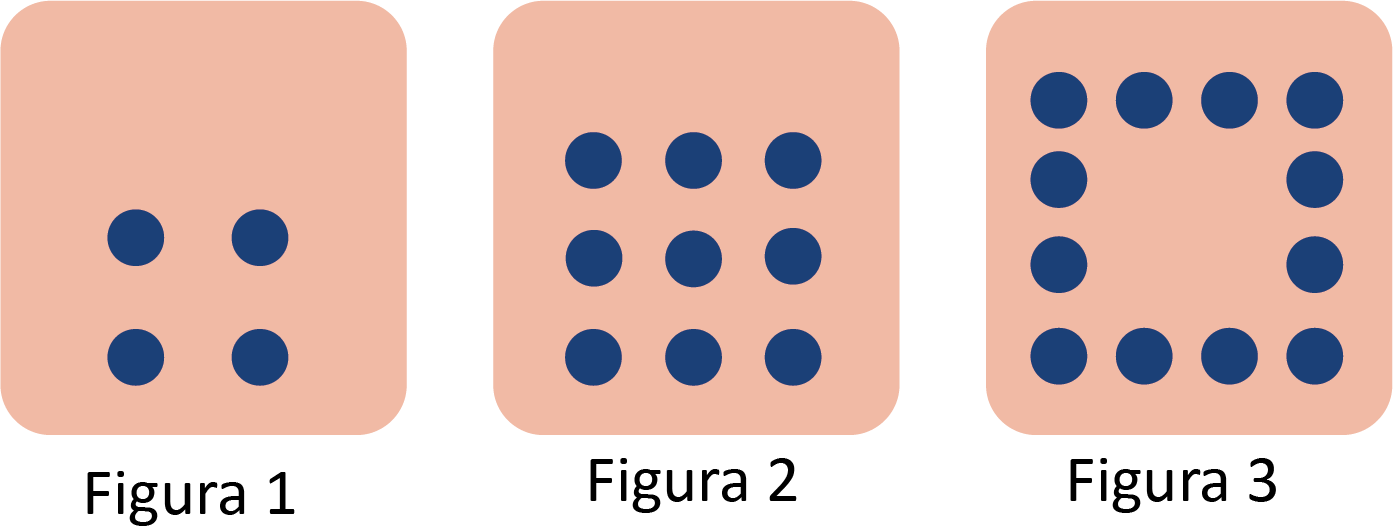
\includegraphics[width=.7\textwidth]{./media/image34.png}
\end{center}
\item \reduline{5; 10; 15; 20; 25; 30; 35 40; ou 5 x 8 = 40.\hfill} bolinhas

\begin{center}

\includegraphics[width=.7\textwidth]{./media/image35.png}
\end{center}
\end{escolha}

\begin{comment}
\num{11} Encontre o número pedido em cada item.

\begin{escolha}
\item O sucessor de 4.089 \reduline{4.090\hfill}

\item O antecessor de 4.302 \reduline{4.301\hfill}

\item O sucessor e o antecessor do número 5.259 \reduline{5.258 e 5.260.\hfill}
\end{escolha}

%\coment{Vale explorar bastante os conceitos de sucessor e antecessor com os alunos, pois isso facilitará muitos entendimentos em anos futuros.}

\num{12} Ana Clara encontrou um papel abaixo entre os cadernos de seu irmão mais velho, com as seguintes anotações:

\begin{myquote}
(21; 58; 95; 132; ...)
\end{myquote}

Ela ficou muito curiosa, pois entendeu que essa era uma sequência
numérica e queria encontrar o próximo número dessa sequência.

Ajude Ana Clara a descobrir qual é o próximo número da sequência e escreva-o no espaço disponível.

\reduline{A sequência foi montada sempre somando 37 ao número anterior para
encontrar o próximo. Portanto, o próximo número da sequência será: 132 + 37 = 169.\hfill}

\num{13} A professora de Camila decidiu propor um desafio à turma. Assim, apresentou uma sequência de figuras e pediu que os alunos descobrissem qual seria a próxima imagem. 

%Usar recortes da imagem disponível em https://br.freepik.com/vetores-gratis/cartoes-de-jogo-de-memoria-desenhados-a-mao_37451777.htm#query=sequ%C3%AAncias%20de%20figuras&position=0&from_view=search&track=robertav1_2_sidr  
%para construir a seguinte sequência:bola-quadrado-quadrado-losango-triângulo-triângulo-triângulo-oval-bola-quadrado-quadrado-losango-triângulo

Quem acertou o desafio foi o colega de Camila, Gabriel. Qual foi a resposta dele?

\reduline{Gabriel respondeu que a próxima figura seria um triângulo.\hfill}

\reduline{É possível que o aluno continue a sequência com desenhos até chegar à resposta. Não há problemas na utilização dessa técnica.\hfill}
\linhas{1}


\num{14} Observe as sequências e complete-as com os números que estão faltando.

\begin{escolha}
\item 102 \quad \reduline{104}\quad 106 \quad \reduline{108} 110 \quad \reduline{112}

\item 85 \quad \reduline{90} \quad \reduline{95} \quad 100 \quad 105 \quad \reduline{110}
\end{escolha}
\end{comment}

\pagebreak

\section*{Treino}

\num{1} Se os números escritos a seguir foram colocados em ordem crescente, qual
é o número que fica imediatamente antes de 63?

\begin{myquote}
\centering
\textbf{95; 63; 25; 76; 54; 68; 48.}
\end{myquote}

\begin{escolha}
\begin{multicols}{2}
% Conteúdo da primeira coluna
\item 25.

\item 48.
\end{multicols}

% Conteúdo entre as duas colunas

\begin{multicols}{2}
% Conteúdo da segunda coluna
\item 54.

\item 68.
\end{multicols}
\end{escolha}

\num{2} Observe a sequência e marque a alternativa que corresponde ao número de bolinhas que a figura 6 terá.

\vspace{1em}
%\begin{figure}[htpb!]
%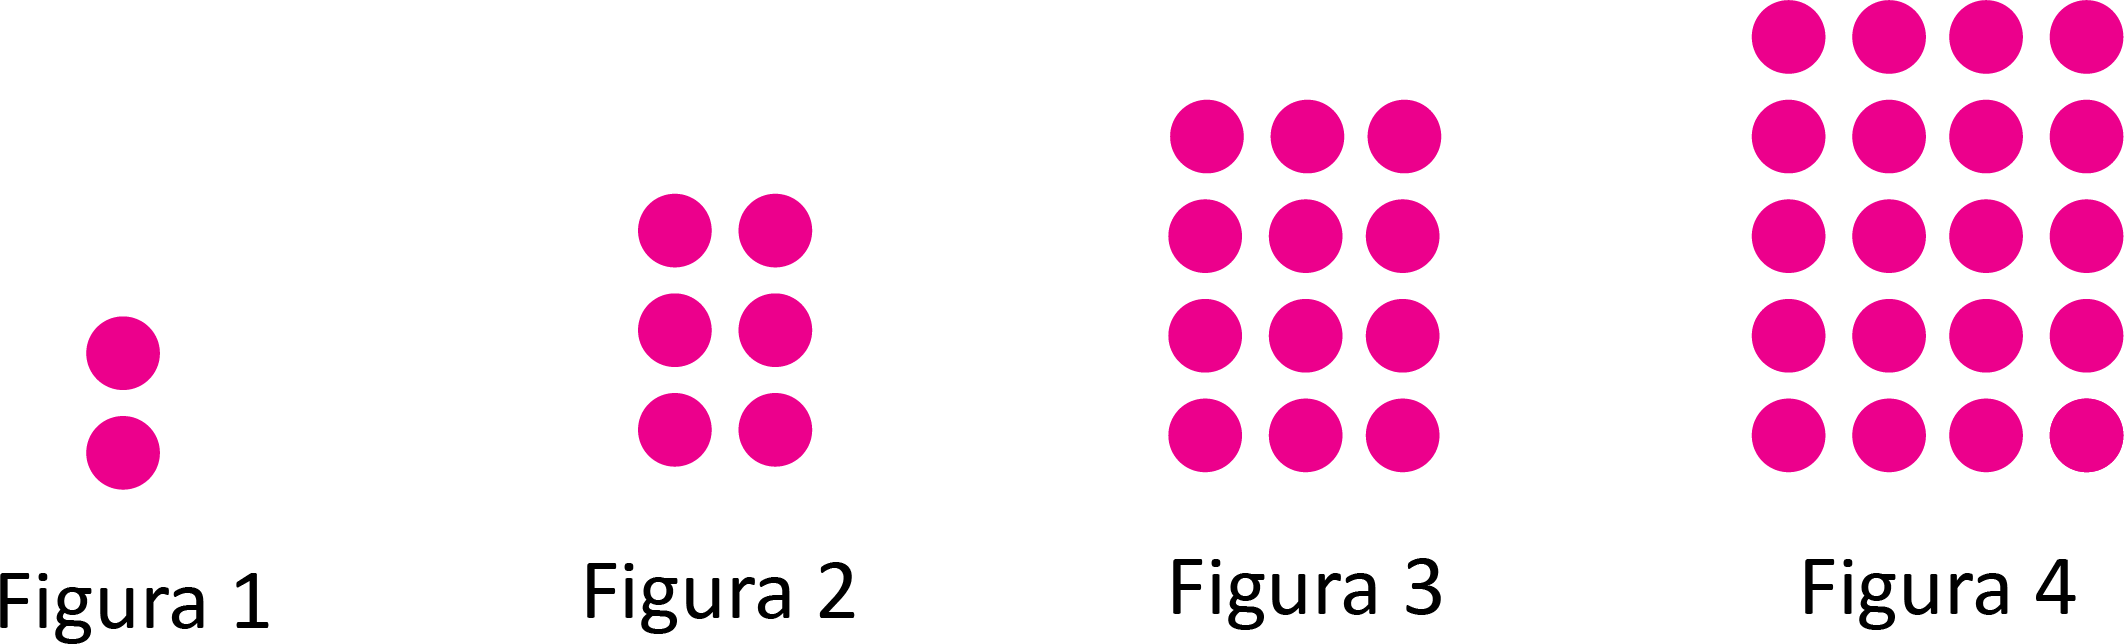
\includegraphics[width=\textwidth]{./media/image37.png}
%\end{figure}

%\item \reduline{4; 7; 10; 13; 16; 19; 22; 25; ou (8 x 3) + 1 = 25.\hfill} bolinhas

\begin{center}
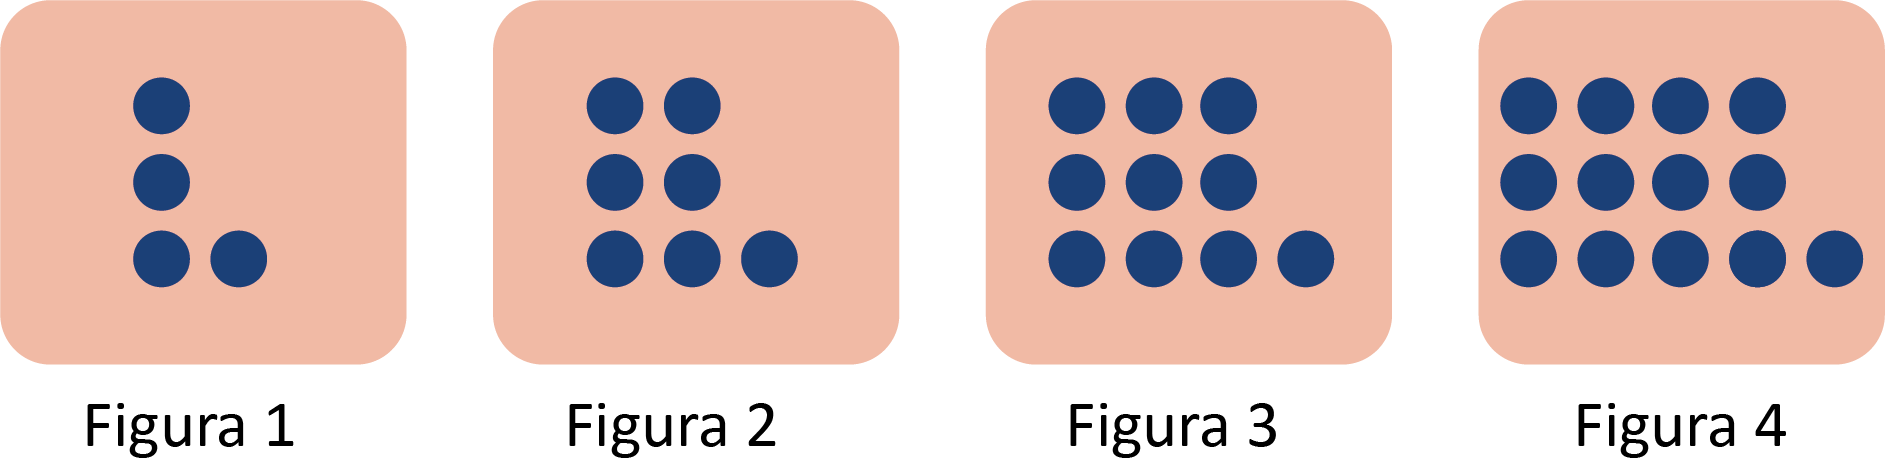
\includegraphics[width=.7\textwidth]{./media/image32.png}
\end{center}

\begin{escolha}

\begin{multicols}{2}
% Conteúdo da primeira coluna

\item 9.

\item 16.
\end{multicols}

% Conteúdo entre as duas colunas

\begin{multicols}{2}
% Conteúdo da segunda coluna

\item 12.

\item 19.
\end{multicols}
\end{escolha}

\num{3} Assinale a alternativa que possui uma sequência que traz um antecessor, um número e seu sucessor.

\begin{escolha}
\item 450; 455; 460.

\item 526; 626; 726.

\item 436; 446; 456.

\item 488; 489; 490.
\end{escolha}

\chapter{Medindo tudo}
\markboth{Módulo 4}{}

\enlargethispage{3\baselineskip}

\section*{Habilidades do SAEB}

\begin{itemize}
\item Reconhecer a unidade de medida ou o instrumento mais apropriado para
medições de comprimento, área, massa, tempo, capacidade ou temperatura.

\item Estimar/inferir medida de comprimento, capacidade ou massa de objetos,
utilizando unidades de medida convencionais ou não ou medir comprimento,
capacidade ou massa de objetos.

\item Explicar que o resultado de uma medida depende da unidade de medida
utilizada.

\item Resolver problemas que envolvam medidas de grandezas (comprimento,
massa, tempo e capacidade) em que haja conversões entre as unidades mais
usuais.

\item Determinar o horário de início, o horário de término ou a duração de
um acontecimento.
\end{itemize}

\subsection{Habilidades da BNCC}

\begin{itemize}
\item EF03MA19, EF03MA20.
\end{itemize}



%\conteudo{
%\noindent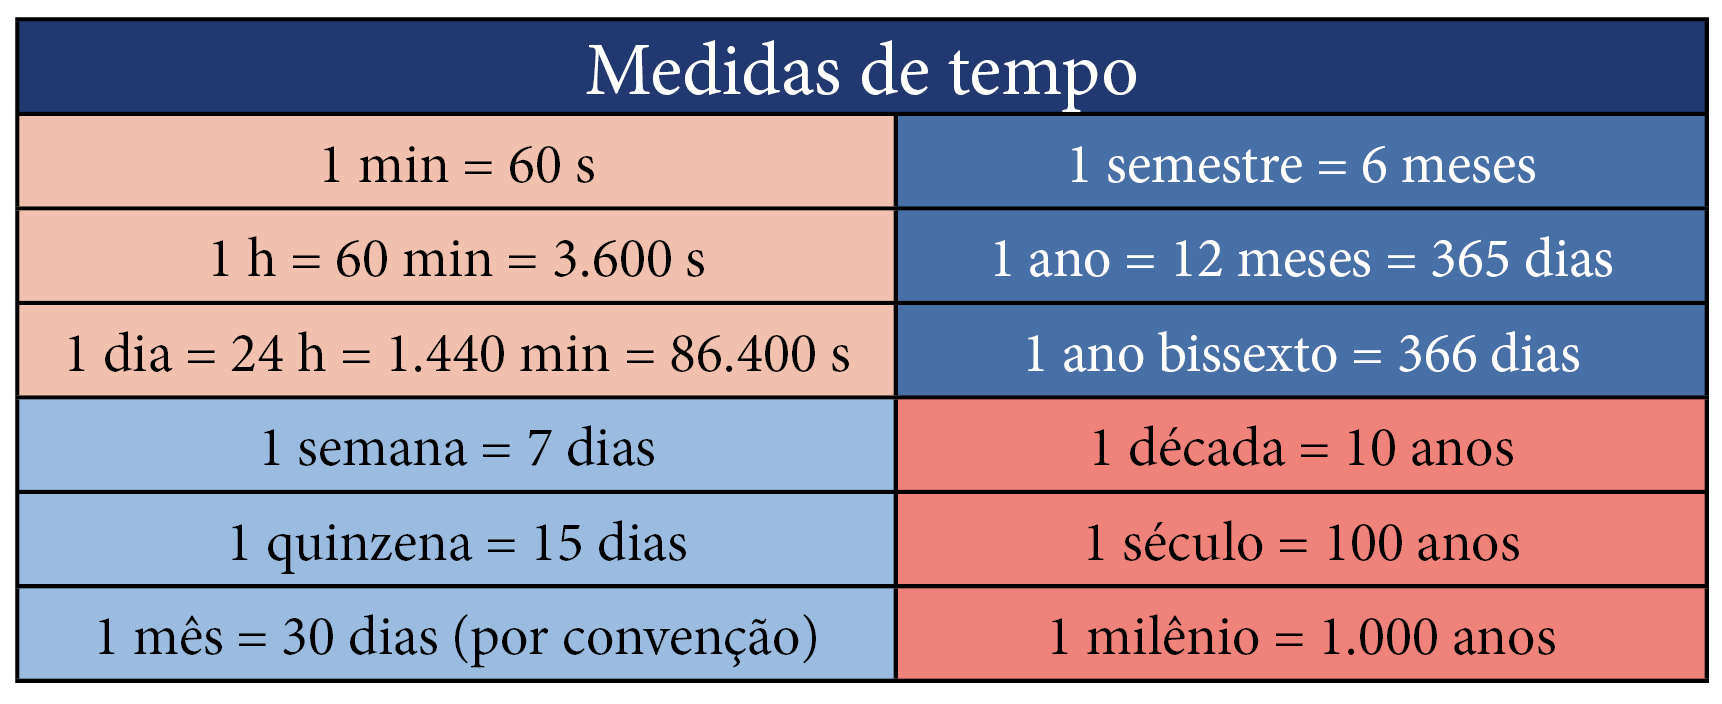
\includegraphics[width=\textwidth]{./media/image39.png}
%} 

\conteudo{
Unidade de medida é uma referência estabelecida para que todos possam medir e comparar grandezas físicas, obtendo os mesmos resultados. Por exemplo, hora, período, dia, semana, mês, ano, década, século, milênio são unidades de medida de tempo.

Observe a tabela a seguir para lembrar das unidades de medida de comprimento, massa e volume.    

\noindent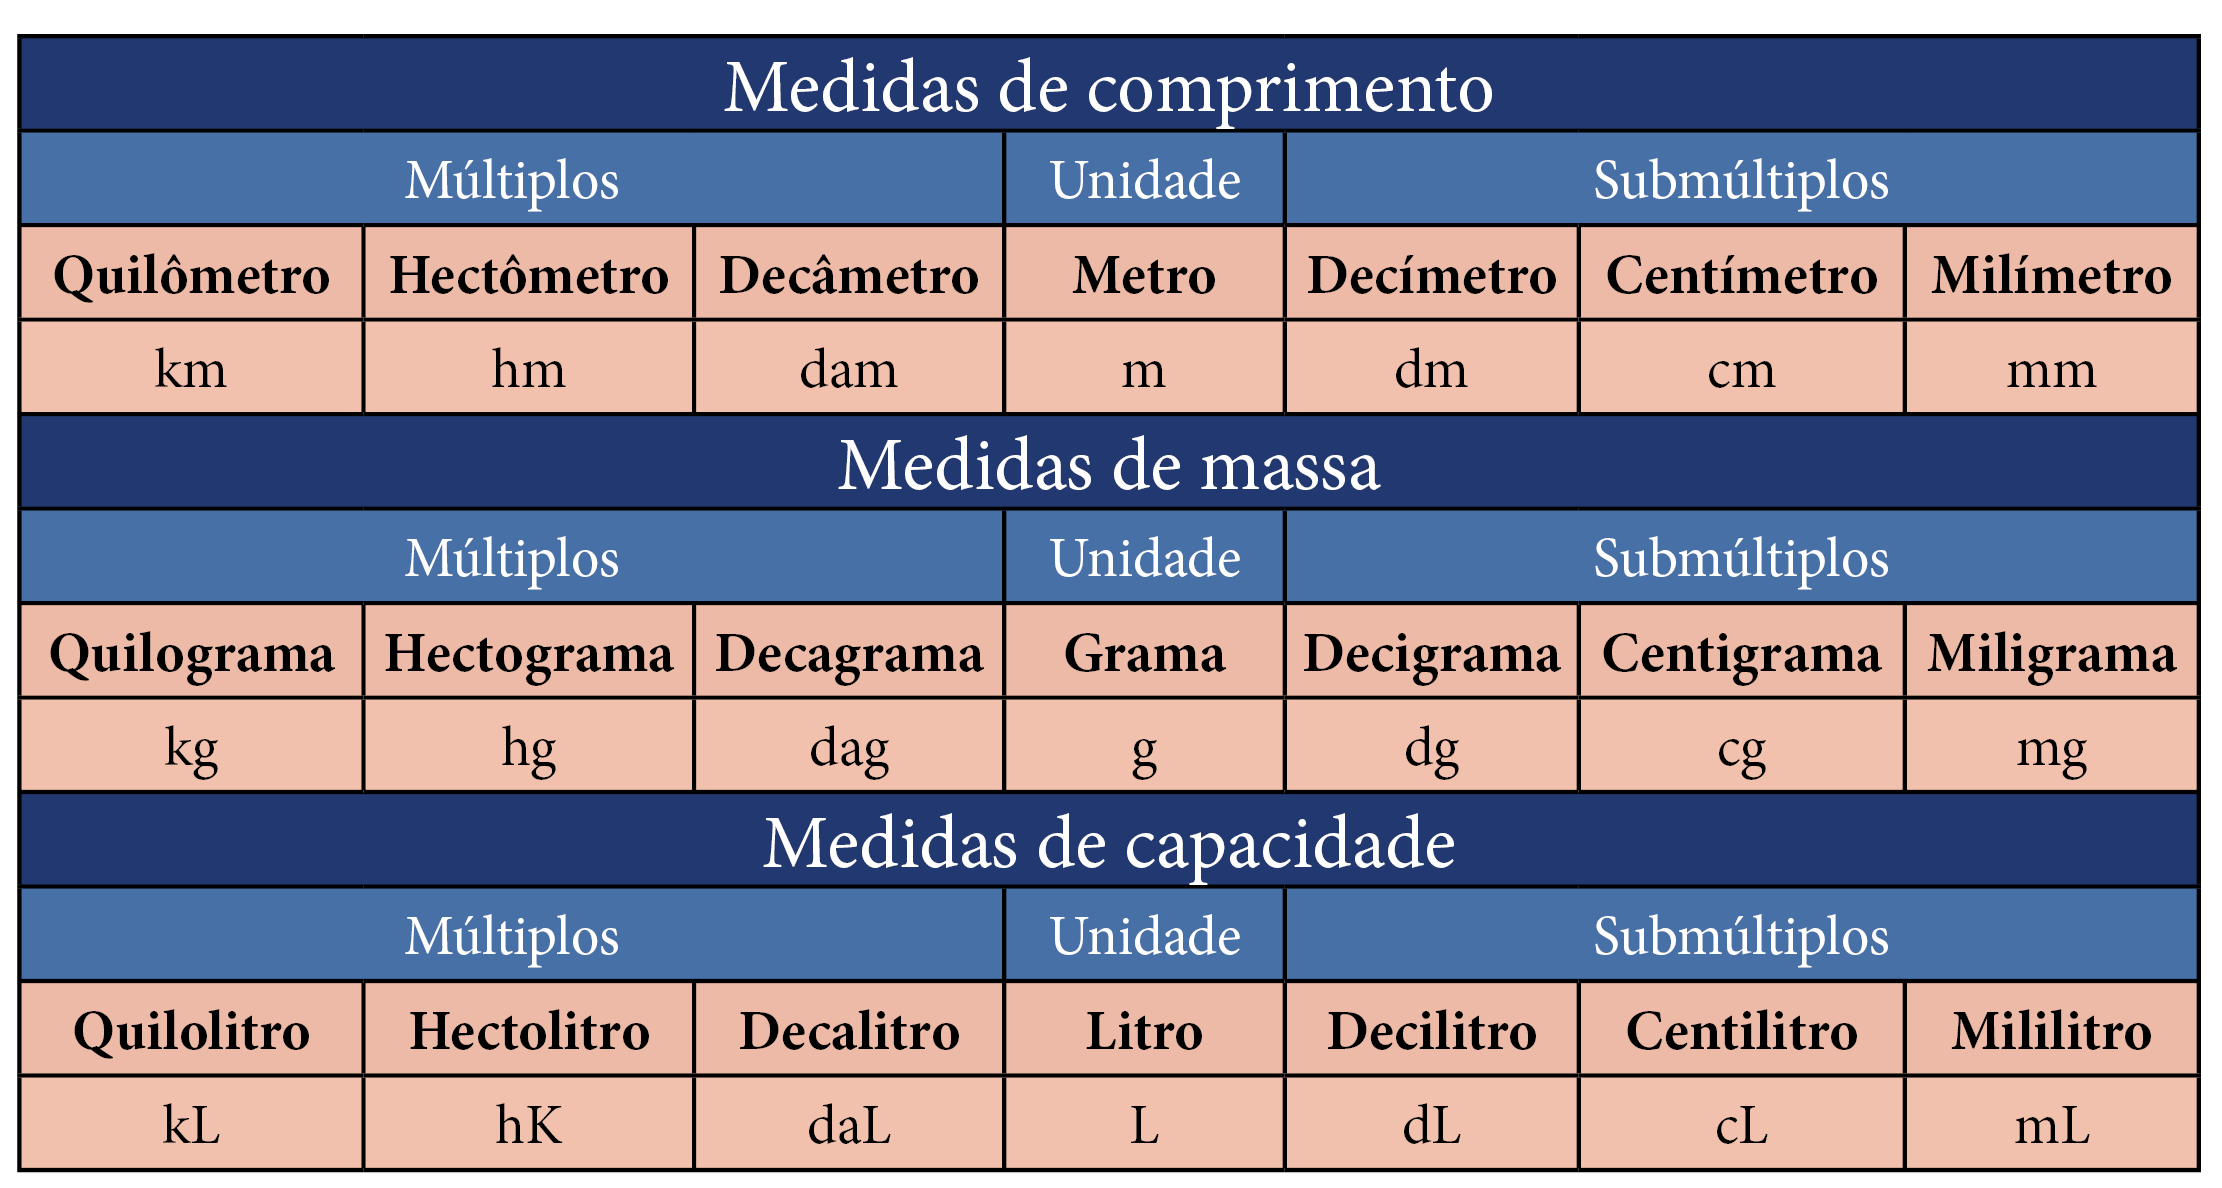
\includegraphics[width=\textwidth]{./media/image38.png}
}

\section*{Atividades}

\num{1} A régua é utilizada para medir comprimento.

\begin{figure}[htpb!]
\centering
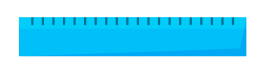
\includegraphics[width=.7\textwidth]{./media/image41a.png}
\end{figure}

\begin{escolha}
\item Escreva o nome de dois objetos da sala de aula que você acredita
  medirem menos de 1 metro.
\reduline{Resposta pessoal.\hfill}
\linhas{2}

\item Escreva o nome de dois objetos da sala de aula que você acredita
  medirem mais de 1 metro.
\reduline{Resposta pessoal.\hfill}
\linhas{2}
\end{escolha}

\num{2} Utilize sua régua para responder aos itens a seguir.

\begin{escolha}
\item Quantos centímetros tem o comprimento da sua borracha?
\reduline{Resposta pessoal.\hfill}

\item Qual é a largura, em centímetros, da carteira que você utiliza na sala de aula?
\reduline{Resposta pessoal.\hfill}

\item Qual é o comprimento, em centímetros, do seu lápis?
\reduline{Resposta pessoal.\hfill}

\item Qual é a altura aproximada de um dos seus colegas?
\reduline{Resposta pessoal.\hfill}
\end{escolha}

\num{3} Relacione a primeira com a segunda coluna, levando em conta qual é valor que 
pode corresponder à cada medida.


\begin{multicols}{2}\parindent=0em
A. Altura aproximada\\
de uma porta\bigskip

B. Comprimento aproximado\\
de um lápis\bigskip

C. Comprimento médio\\
de um quarteirão\bigskip

D. Comprimento aproximado de\\
uma quadra de basquete

\columnbreak

(\hspace{2em}) 20 cm\bigskip

(\hspace{2em}) 90 m\bigskip

(\hspace{2em}) 30 m\bigskip

(\hspace{2em}) 2 m
\end{multicols}


\coment{Resposta: B, C, D, A.}

\pagebreak

\num{4} Complete a frase com o número que representa quanto mede cada um dos
objetos indicados a seguir.

\begin{escolha}

\item O lápis mede \reduline{9 cm.\hfill}

\begin{center}
\noindent
\includegraphics[width=0.8\textwidth]{./media/image42.png}
\end{center}

\item A borracha mede \reduline{6 cm.\hfill}

\begin{center}
\noindent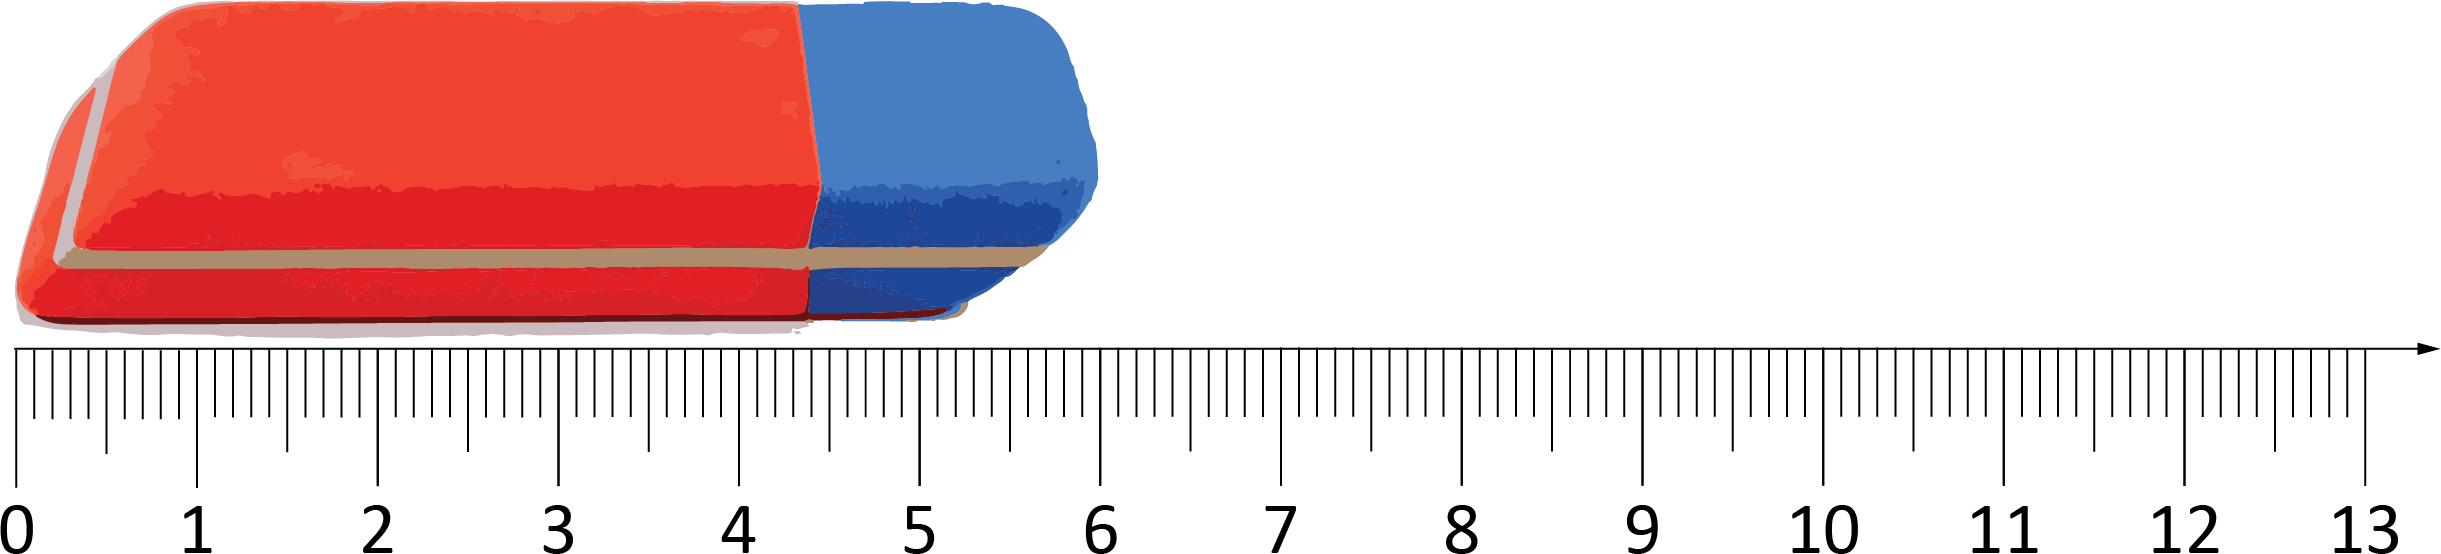
\includegraphics[width=0.6\textwidth]{./media/image43.png}
\end{center}

\item O apontador mede \reduline{4 cm.\hfill}

\begin{center}
\noindent
\includegraphics[width=0.6\textwidth]{./media/image44.png}
\end{center}

\item A tesoura mede \reduline{11 cm.\hfill}

\begin{center}
\noindent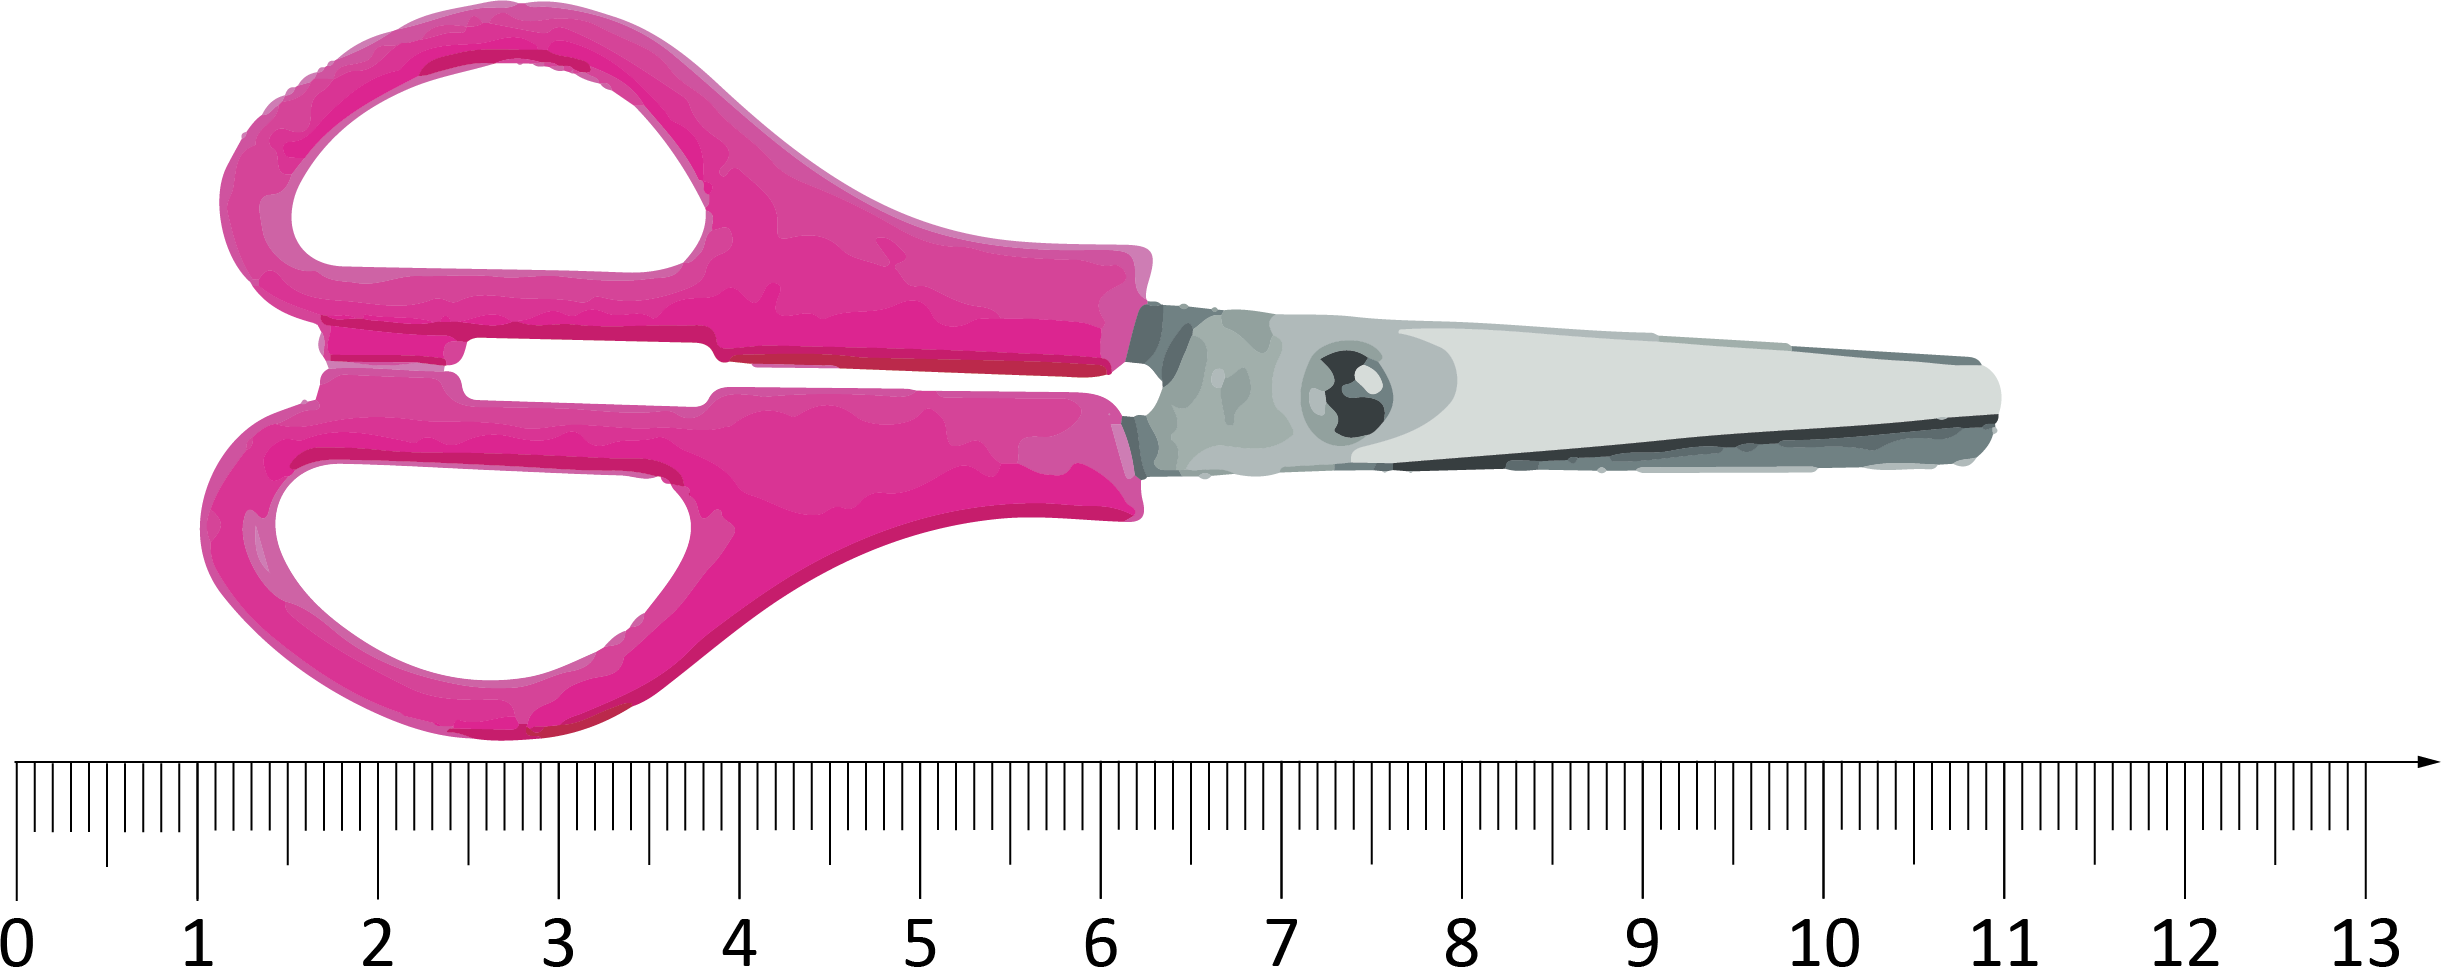
\includegraphics[width=0.6\textwidth]{./media/image45.png}
\end{center}
\end{escolha}

%\coment{Vale a pena explorar bastante essa questão de medir com o auxílio da reta numérica, principalmente quando o início não é no zero. Esse conceito é muito útil para entendimento de assuntos que virão em outros anos e trabalhar bastante agora pode ajudar muito o aluno em anos posteriores.}

\pagebreak
\num{5} Débora decidiu estimar a medida do seu lápis com sua borracha.

\begin{figure}[htpb!]
\centering
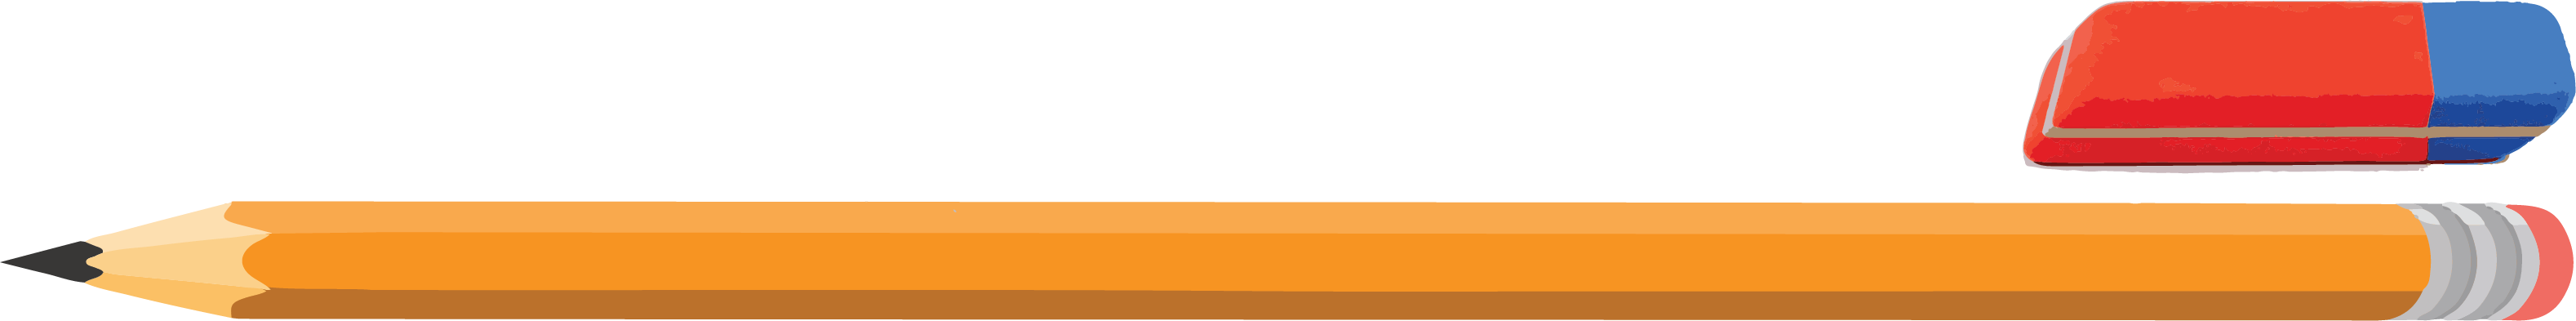
\includegraphics[width=.5\textwidth]{./media/image46.png}
\end{figure}

Quantas borrachas, aproximadamente, mede o lápis de Débora, considerando a figura dada?

\reduline{ Por comparação, pode-se estimar que no comprimento do lápis cabem cerca de 4 a 5 borrachas, conforme a figura dada.\hfill}
\linhas{2}

\num{6} Um dos brinquedos do parque de diversões permanente de uma cidade proíbe
que crianças com altura menor que 1,30 m possam brincar nessa
atração. Manoel mediu sua altura e ele está com 93 cm. Quanto ele
precisa crescer para poder realizar seu sonho de andar nesse brinquedo?
\reduline{1,30 m = 130 cm; 130 -- 93 = 33 cm. Portanto, ele ainda precisará crescer 33 cm para poder usar o brinquedo.\hfill}
\linhas{2}

\num{7} Roberto está com sintomas de dor de garganta, e sua mãe o levou ao
médico. Quando chegou ao consultório, sua temperatura foi medida, como indicado na fotografia a seguir.

\begin{figure}[htpb!]
\centering
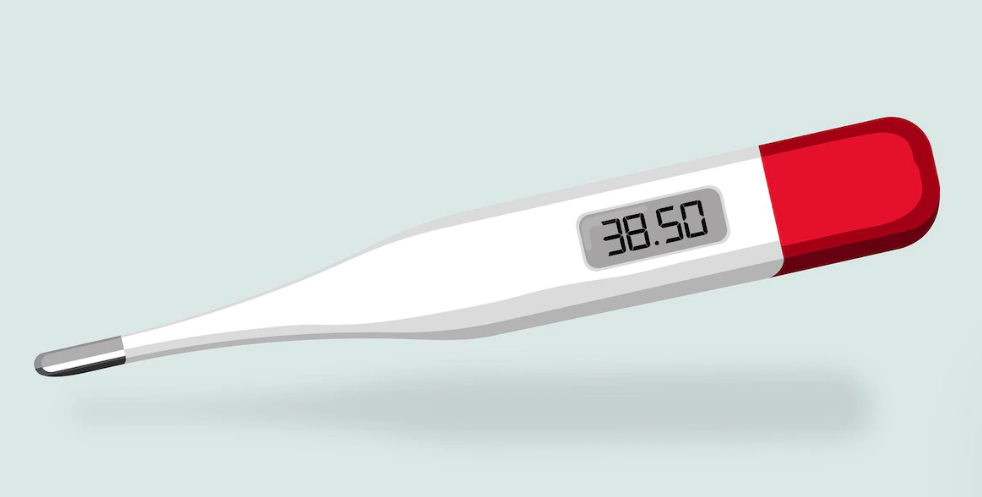
\includegraphics[width=.5\textwidth]{./media/image47.png}
\end{figure}

\begin{escolha}
\item Analisando a imagem do termômetro, qual a temperatura de Roberto nesse instante?
\reduline{38,5º C.\hfill}
\end{escolha}

\num{8} O pai de Arthur encomendou 24 garrafas de
refrigerante para a festa de aniversário do filho. Dessas garrafas, 10 tinham capacidade de 3 litros cada uma delas. As demais garrafas tinham capacidade de 2 litros cada. Com base nessas
informações, responda ao que se pede a seguir.

\begin{figure}[htpb!]
\centering
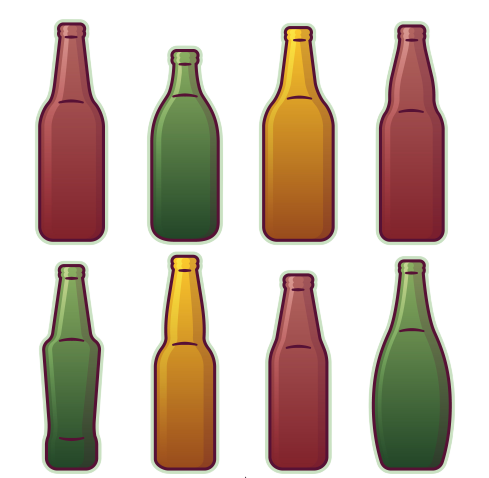
\includegraphics[width=.6\textwidth]{./media/image47a.png}
\end{figure}

\begin{escolha}
\item Qual a quantidade, em mililitros, encomendada pelo pai de Arthur?
\reduline{(10 x 3) + (14 x 2) = 30 + 28 = 58 L = 58.000 ml\hfill}
\linhas{1}

\item Se cada pessoa consumiu exatamente 400 mililitros de refrigerante e
  todo o refrigerante foi consumido durante a festa, quantas pessoas
  foram ao aniversário de Arthur?
\reduline{58.000 : 400 = 145 pessoas compareceram à festa.\hfill}
\linhas{2}
\end{escolha}

\num{9} O comprimento de uma escrivaninha é de 1,6 m. 

\begin{figure}[htpb!]
\centering
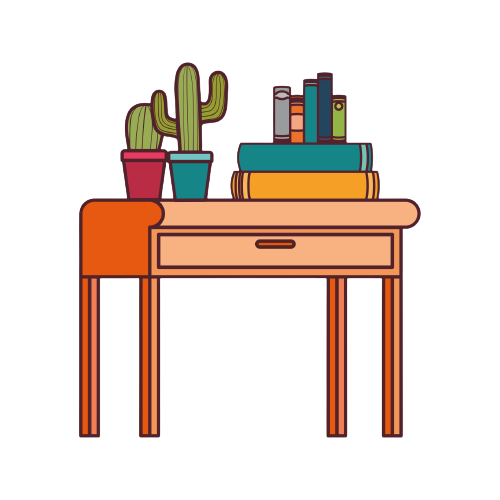
\includegraphics[width=.5\textwidth]{./media/image47b.png}
\end{figure}

\begin{escolha}
\item Quantos palmos,
aproximadamente, mede a escrivaninha se, em média, um palmo tem 23 cm?
\reduline{1,6 m = 160 cm; 160 : 23 = 6,95 palmos. Aproximadamente 7 palmos.\hfill}\linhas{2}
\end{escolha}

\num{10} Os episódios de uma série de televisão têm 45 minutos de duração.
Se Jorge terminou de assistir a um episódio às 17 horas, qual foi o
horário em que ele começou a assistir ao episódio, considerando que não houve interrupções?
\reduline{Jorge começou a assistir ao episódio às 16h15.\hfill}\linhas{1}
\linhas{2} 

\pagebreak
\section*{Treino}

\num{1} Reinaldo foi contratado por uma empresa que exige que se cumpra os horários exatamente como mostra o contrato. No período da manhã, ele deve
cumprir 4 horas e 30 minutos de trabalho. Qual será o horário que
Reinaldo sairá para almoçar?

\begin{longtable}[]{@{}lll@{}}
\toprule
& \textbf{Entrada} & \textbf{Saída}\tabularnewline
\midrule
\endhead
\hline
\textbf{Manhã} & 8:00 & ?\tabularnewline
\hline
\textbf{Tarde} & 14:00 & 17:30\tabularnewline
\hline
\bottomrule
\end{longtable}

\begin{escolha}
\begin{multicols}{2}
% Conteúdo da primeira coluna

\item 11h00.

\item 11h30.
\end{multicols}

% Conteúdo entre as duas colunas

\begin{multicols}{2}
% Conteúdo da segunda coluna

\item 12h00.

\item 12h30.
\end{multicols}
\end{escolha}


\num{2} Júlia está com tosse, e sua avó preparou para ela um chá de menta com mel, ótimo para resolver o problema. A avó colocou o chá na geladeira em garrafinhas de 500 mL. Se Júlia tomar um copinho de 40 mL, 4 vezes ao dia, por dez dias, quantas garrafinhas precisarão ser preparadas pela avó?

\begin{escolha}
\begin{multicols}{2}
% Conteúdo da primeira coluna

\item 1.

\item 2.
\end{multicols}

% Conteúdo entre as duas colunas

\begin{multicols}{2}
% Conteúdo da segunda coluna

\item 3.

\item 4.
\end{multicols}
\end{escolha}


\num{3} Luana foi visitar sua avó, que mora em outro estado. Seu voo
saiu do aeroporto às 8 horas e 15 minutos e chegou ao seu destino às 11
horas e 30 minutos. Calcule o tempo de duração do voo.

\begin{escolha}
\begin{multicols}{2}
% Conteúdo da primeira coluna

\item 3 horas e 15 minutos.

\item 2 horas.
\end{multicols}

% Conteúdo entre as duas colunas

\begin{multicols}{2}
% Conteúdo da segunda coluna

\item 2 horas e 45 minutos.

\item 3 horas e 50 minutos.
\end{multicols}  
\end{escolha}

\chapter{Tempo e comprimento}
\markboth{Módulo 5}{}\enlargethispage{6\baselineskip}

\vspace*{-1.5cm}

\section*{Habilidades do SAEB}

\begin{itemize}
\item Medir ou comparar perímetro ou área de figuras planas desenhadas em malha quadriculada.

\item Identificar horas em relógios analógicos ou associar horas em relógios analógicos e digitais.

\item Resolver problemas que envolvam perímetro de figuras planas.

\item Resolver problemas que envolvam área de figuras planas.
\end{itemize}

\subsection{Habilidades da BNCC}

\begin{itemize}
 \item  EF03MA22, EF03MA23.
\end{itemize}


\conteudo{
Um dia dura 24 horas.

Uma semana é composta por 7 dias.   

\begin{myquote}
Os dias da semana são:
\begin{flushleft}
\textbf{domingo, segunda-feira, terça-feira, quarta-feira, quinta-feira, sexta-feira e sábado.}
\end{flushleft}
\end{myquote}

Um ano é composto por 12 meses. O nome dos meses e suas respectivas quantidades de dias estão na tabela a seguir.

\pagebreak

\begin{myquote}
\begin{small}
\begin{longtable}[]{@{}ll@{}}
\toprule
\textbf{Meses que compõem o ano} & \textbf{Número de dias dos meses}\tabularnewline
\midrule
\endhead
Janeiro & 31\tabularnewline
Fevereiro & 28 (em ano bissexto tem 29 dias)\tabularnewline
Março & 31\tabularnewline
Abril & 30\tabularnewline
Maio & 31\tabularnewline
Junho & 30\tabularnewline
Julho & 31\tabularnewline
Agosto & 31\tabularnewline
Setembro & 30\tabularnewline
Outubro & 31\tabularnewline
Novembro & 30\tabularnewline
Dezembro & 31\tabularnewline
\bottomrule
\end{longtable}
\end{small}
\end{myquote}
}

\conteudo{
O relógio analógico é um instrumento de medição de tempo. 
Ele recebe esse nome porque originalmente seu mecanismo 
era movido por corda. Atualmente, muitos relógios de ponteiros 
utilizam energia de uma bateria para funcionar. 
Ele pode indicar unidades de tempo como dia, hora, minuto e segundo.

O mostrador do relógio analógico é dividido em partes iguais, numeradas de 1 a 12. Esses números representam as horas. 

O espaço entre um número e o próximo número representa os minutos e corresponde a 5 minutos.  


Em geral, o ponteiro menor indica as horas; o ponteiro médio, os minutos; e o ponteiro maior, os segundos.  

Para ler as horas no relógio analógico, siga a ordem: primeiro, o ponteiro das horas, e, depois, o ponteiro dos minutos. 
\begin{myquote}
\begin{itemize}

\item Observe o exemplo a seguir. O ponteiro menor está no 11, e o ponteiro maior, no 12. Então, são onze horas. 

\end{itemize}
\end{myquote}

\begin{center}
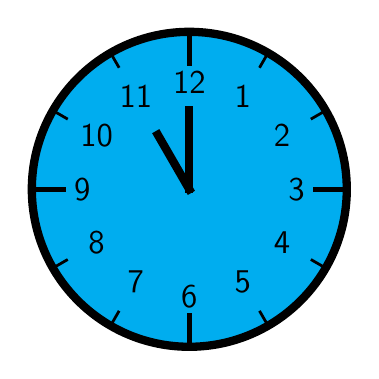
\begin{tikzpicture}[line cap=rect,line width=3pt]
\filldraw [fill=cyan] (0,0) circle [radius=2cm];
\foreach \angle [count=\xi] in {60,30,...,-270}
{
  \draw[line width=1pt] (\angle:1.8cm) -- (\angle:2cm);
  \node[font=\large] at (\angle:1.36cm) {\textsf{\xi}};
}
\foreach \angle in {0,90,180,270}
  \draw[line width=2pt] (\angle:1.6cm) -- (\angle:2cm);
\draw (0,0) -- (120:0.8cm);
\draw (0,0) -- (90:1cm);
\end{tikzpicture}
\end{center}
}

\section*{Atividades}

\num{1} Observe os horários nos relógios representados.

\begin{figure}[htpb!]
\includegraphics[width=\textwidth]{./media/image51.png}
\end{figure}

Qual o horário cada relógio está marcando?
\reduline{Estão representadas sete horas no primeiro relógio; sete e meia ou sete horas e trinta minutos no segundo relógio; e meio-dia e quinze minutos ou doze horas e quinze minutos no terceiro relógio.\hfill}
\linhas{2}

\pagebreak

\num{2} Observe o horário que os relógios digitais estão marcando:

\begin{figure}[htpb!]
\includegraphics[width=\textwidth]{./media/image52.png}
\end{figure}

Como se lê cada um dos horários marcados?
\reduline{Estão representadas nove e meia ou nove horas e trinta minutos no primeiro relógio; meio-dia ou doze horas no primeiro relógio; e cinco horas no terceiro relógio.\hfill}
\linhas{1}

\num{3} A professora de Francisco colocou como primeira questão da prova a seguinte imagem:

\begin{figure}[htpb!]
\centering
\includegraphics[width=\textwidth]{./media/image53.png}
\end{figure}

Ajude Francisco a completar os retângulos em branco com indicação de
minutos que cada um deles aponta.

\coment{20 minutos; 35 minutos; 40 minutos; 45 minutos; 55 minutos; 60 minutos.}

\pagebreak

\num{4} Observe o calendário e em seguida responda aos itens propostos.

\begin{figure}[htpb!]
\centering
\includegraphics[width=\textwidth]{./media/image54.png}
\end{figure}

\pagebreak
\begin{escolha}
\item Circule no calendário o dia de seu aniversário.
%\reduline{Resposta pessoal.\hfill}

\item Agora, com um retângulo, marque o dia do aniversário de três colegas da sua sala.
%\reduline{Resposta pessoal.\hfill}

\item Marque com um triângulo o dia do aniversário de seu professor.
%\reduline{Resposta pessoal.\hfill}

\item Quantos anos você tem?
\reduline{Resposta pessoal.\hfill}

\item Você tem mais ou menos de 450 meses?
\reduline{Resposta pessoal.\hfill}
\end{escolha}

\num{5} O pai de Rafael estava conversando com um contador sobre o seu
faturamento semestral. Rafael escutou toda a conversa e depois fez os
seguintes questionamentos a seu pai:

O que é um semestre? 
Quantos semestres temos em um ano?

Diante de tantas perguntas, o pai de Rafael sentou-se com seu filho e
começou a responder aos questionamentos do filho.

Ajude o pai de Rafael a responder corretamente a todas as perguntas que o filho lhe fez.
\reduline{Um semestre é um período composto por 6 meses e em um ano temos 2 semestres.\hfill}

\num{6} Marque, desenhando no relógio analógico abaixo, os ponteiros das horas e o dos
minutos na posição exata em que estarão para representar o horário em que
suas aulas começam.

\begin{figure}[htpb!]
\centering
\includegraphics[width=0.3\textwidth]{./media/image54b.png}
\end{figure}

\coment{Resposta circunstancial. Dependerá do horário de início das aulas.}

\pagebreak

\num{7} Aos finais de semana, Renato anda de bicicleta ao redor da praça do bairro onde mora.

\begin{figure}[htpb!]
\centering
\includegraphics[width=.4\textwidth]{./media/image55.png}
\end{figure}

Se ele der duas voltas completas ao redor da praça, qual é a distância que ele percorrerá?

\reduline{(2 x 30 + 2 x 50) x 2 = 320 m. Sempre que possível, estimule a montagem da expressões, para que os alunos comecem a se acostumar.\hfill}
\linhas{1}

\num{8} As figuras a seguir foram desenhadas em uma malha quadriculada.

\begin{figure}[htpb!]
\centering
\includegraphics[width=0.5\textwidth]{./media/image56.png}
\end{figure}

Quantos quadradinhos pintados cada figura possui?
\reduline{Verde: 21 quadradinhos; azul: 24 quadradinhos; e laranja: 9 quadradinhos.\hfill}
\linhas{1}

\num{9} Na malha quadriculada, cada quadrado representa uma área de 10 metros quadrados.

\begin{figure}[htpb!]
\centering
\includegraphics[width=.6\textwidth]{./media/image60.png}
\end{figure}

Qual é a área que a figura ocupa na malha quadriculada?
\reduline{Realizando a contagem de quadradinhos que preenchem a figura, chega-se à conclusão de que, para o preenchimento dela, são necessários 16 quadradinhos. Portanto, 16 x 10 = 160 metros quadrados.\hfill}

\vspace{2em}

\begin{comment}
\num{10} Os desenhos representados foram feitos com o auxílio de uma malha
quadriculada na qual cada lado de quadradinho mede 1 cm.

\begin{figure}[htpb!]
\includegraphics[width=\textwidth]{./media/image57.png}
\end{figure}

\begin{escolha}
\item Qual a medida, em centímetros, do contorno da figura azul?
\reduline{18 cm\hfill}

\item Qual a medida, em centímetros, do contorno da figura amarela?
\reduline{12 cm\hfill}

\item Qual a medida, em centímetros, do contorno da figura verde?
\reduline{22 cm\hfill}
\end{escolha}
\end{comment}

\num{10} Utilizando sua régua, una pontos e faça uma figura na malha, representada apenas pelos pontinhos. Em seguida, mostre sua
figura para um colega e veja se ele descobre o que você representou.

\begin{figure}[htpb!]
\includegraphics[width=\textwidth]{./media/image58.png}
\end{figure}

\coment{Resposta pessoal.}

\begin{comment}
\num{11} Observe atentamente as figuras.

\begin{figure}[htpb!]
\centering
\includegraphics[width=.6\textwidth]{./media/image59.png}
\end{figure}

Quais delas possuem a mesma quantidade de quadradinhos? Justifique sua resposta.
\reduline{Todas são compostas pelo mesmo número de quadradinhos.\hfill}
\linhas{2}
\end{comment}

\section*{Treino}

\num{1} Paulo resolveu ir a uma exposição e, no momento, encontra-se na
bilheteria. Quanto ele precisará andar para chegar à exposição,
considerando o caminho destacado, sabendo-se que o lado de cada
quadradinho da malha tem medida de 3m?

\begin{figure}[htpb!]
\includegraphics[width=\textwidth]{./media/image61.png}
\end{figure}

\begin{escolha}
\item
  5 m.
\item
  10 m.
\item
  12 m.
\item
  15 m.
\end{escolha}

\pagebreak

\num{2} Amanda quer fazer seu nome em letras bem grandes em um papel colorido para enfeitar sua festa de aniversário. Para as letras terem tamanhos equivalentes, resolveu, primeiro, desenhá-las em um papel quadriculado. Veja o A que ela fez.

Quantos quadrados, de forma aproximada, esse A ocupa?

\begin{figure}[htpb!]
\centering
\includegraphics[width=.8\textwidth]{./media/image62.png}
\end{figure}

\begin{escolha}
\item
  3.
\item
  9.
\item
  26.
\item
  120.
\end{escolha}

\pagebreak
\num{3} Leia a notícia.

\begin{quote}
A cidade de Tombalina ganhará uma nova praça. A praça atual, com a famosa pista de corrida de 25 metros, será substituída por outra, com pista de corrida e caminhada de 125 metros de comprimento.

A nova praça será construída no centro da cidade, em uma área verde que atualmente não está sendo utilizada. A prefeitura investirá na criação de um espaço amplo e agradável para a população, com áreas de lazer e convivência.

\vspace{1em}
\begin{center}
\includegraphics[width=0.5\textwidth]{./media/image62a.jpeg}
\end{center}
\vspace{1em}

De acordo com o prefeito da cidade, a nova praça é um importante espaço de lazer para a cidade. ``Estamos investindo em espaços públicos de qualidade para a população, que poderá desfrutar de um ambiente agradável e seguro para passear, praticar atividades físicas e aproveitar o tempo livre'', afirmou ele.

A obra está prevista para começar em breve e deve ser concluída em alguns meses. A prefeitura pede a colaboração da população para evitar o desperdício de água e para cuidar do novo espaço, para que todos possam desfrutar de um local agradável e bonito por muitos anos.

\fonte{Texto escrito especialmente para o material.}
\end{quote}

Lendo a notícia, pode-se concluir que a nova pista será \_\_\_\_\_\_\_ em relação à anterior.

\begin{escolha}
\begin{multicols}{2}
\item
  2 vezes maior
\item
  3 vezes maior
\item
  4 vezes maior
\item
  5 vezes maior
  \end{multicols}
\end{escolha}

\chapter{Nosso dinheiro}
\markboth{Módulo 6}{}

\section*{Habilidades do SAEB}

\begin{itemize}
\item Relacionar valores de moedas e/ou cédulas do sistema monetário
brasileiro, com base nas imagens desses objetos.

\item Resolver problemas que envolvam moedas e/ou cédulas do sistema
monetário brasileiro.
\end{itemize}

\subsection{Habilidade da BNCC}

\begin{itemize}
  \item 
 EF03MA24.
\end{itemize}

\conteudo{
\begin{center}
\includegraphics[width=.5\textwidth]{./media/image64.png}
\end{center}}
%NOTE. IMAGEM COM FUNDO.

\pagebreak

\section*{Atividades}

\begin{comment}
\num{1} Complete o quadro, relacionando o valor das cédulas e moedas do
sistema monetário brasileiro com seu valor e com como se lê esse valor.

\begin{longtable}[]{@{}lll@{}}
\toprule
\hline
\vspace{1em}
\textbf{Cédula ou moeda} & \textbf{Valor} & \textbf{Como se lê}\tabularnewline
\hline
\midrule
\endhead
\vspace{1em}
Nota de 200 reais & \rosa{R\$ 200,00} & Duzentos reais\tabularnewline
\hline
\vspace{1em}
Nota de 100 reais & \rosa{R\$ 100,00} & \rosa{Cem reais}\tabularnewline
\hline
\vspace{1em}
Nota de 50 reais & \rosa{R\$ 50,00} & \rosa{Cinquenta reais}\tabularnewline
\hline
\vspace{1em}
Nota de 20 reais & R\$ 20,00 & \rosa{Vinte reais}\tabularnewline
\hline
\vspace{1em}
Nota de 10 reais & \rosa{R\$ 10,00} & \rosa{Dez reais}\tabularnewline
\hline
\vspace{1em}
Nota de 5 reais & \rosa{R\$ 5,00} & Cinco reais\tabularnewline
\hline
\vspace{1em}
Nota de 2 reais & \rosa{R\$ 2,00} & \rosa{Dois reais}\tabularnewline
\hline
\vspace{1em}
Moeda de 1 real & \rosa{R\$ 1,00} & \rosa{Um real}\tabularnewline
\hline
\vspace{1em}
Moeda de 0,50 centavos & R\$ 0,50 & \rosa{Cinquenta
centavos}\tabularnewline
\hline
\vspace{1em}
Moeda de 0,25 centavos & \rosa{R\$ 0,25} & \rosa{Vinte e cinco
centavos}\tabularnewline
\hline
\vspace{1em}
Moeda de 0,10 centavos & \rosa{R\$ 0,10} & \rosa{Dez centavos}\tabularnewline
\hline
\vspace{1em}
Moeda de 0,05 centavos & \rosa{R\$0,05} & Cinco centavos\tabularnewline
\hline
\bottomrule
\end{longtable}
\end{comment}

\num{1} André foi ao banco efetuar um saque (retirada de dinheiro de sua conta
bancária) e, ao pegar o valor pretendido, recebeu as seguintes cédulas e moedas:

\begin{figure}[htpb!]
\centering
\includegraphics[width=\textwidth]{./media/image65.png}
\end{figure}

Qual o valor que André retirou de sua conta bancária?
\reduline{1 x 50 + 4 x 20 + 1 x 10 + 3 x 5 + 2 x 2 + 2 x 1 + 5 x 0,50 = 50 + 80 +
10 + 15 + 4 + 2 + 2,5 = R\$ 163,50.\hfill}
\linhas{4}

\pagebreak
\num{2} A mãe de Leonardo foi ao supermercado. Ela comprou um pacote de açúcar mascavo, três unidades de suco, um pacote de arroz integral, um queijo, uma manteiga e um pacote de café.

Observando o preço de cada produto e a quantidade que ela adquiriu, qual é o valor que ela gastou? 

\begin{figure}[htpb!]
\centering
\includegraphics[width=\textwidth]{./media/image66.png}
\end{figure}

\reduline{Açúcar mascavo: 1 x R\$: 5,00; suco: 3 x R\$ 3 = R\$ 9,00; arroz integral: 1 x R\$ 10,00; queijo: 1 x R\$ 19,00; manteiga: R\$ 15,00; café: R\$ 9,00. Valor total: 5 + 9 + 10 + 19 + 15 + 9 = R\$ 67,00.}

\num{3} Uma grande rede de lojas realizou uma promoção de vendas após o Natal.
Veja os produtos que estavam em promoção e seus respectivos preços.

\begin{figure}[htpb!]
\centering
\includegraphics[width=.73\textwidth]{./media/image67.png}
\end{figure}

\pagebreak

Observavdo a figura, responda a cada item.

\begin{escolha}
\item Se uma pessoa comprar um fogão e um liquidificador, quanto irá pagar?
\reduline{1.300 + 250 = R\$ 1.550,00.\hfill}

\item Se uma pessoa conseguir um desconto de R\$ 50,00 para pagamento à
  vista na compra do microondas, qual será o valor que ela pagará?
\reduline{480 - 50 = R\$ 430,00.\hfill}
\end{escolha}

\num{4} O quadro a seguir mostra a pesquisa de preços que José está fazendo
de um jogo de videogame e um controle bluetooth.

\begin{longtable}[]{@{}lll@{}}
\toprule
\hline
\textbf{Produto} & \textbf{Loja A} & \textbf{Loja B}\tabularnewline
\hline
\midrule
\endhead
\textbf{Jogo de videogame} & R\$ 200,00 & R\$ 176,00\tabularnewline
\hline
\textbf{Controle bluetooth} & R\$ 616,00 & R\$ 654,00\tabularnewline
\hline
\hline
\textbf{Total} & \textbf{R\$} & \textbf{R\$}\tabularnewline
\bottomrule
\end{longtable}

\begin{figure}[htpb!]
\centering
\includegraphics[width=.6\textwidth]{./media/image67a.png}
\end{figure}

\begin{escolha}
\item Se José comprar os dois itens na loja A, pagará quanto?
\reduline{200 + 616 = R\$ 816,00\hfill}

\item Se optar por comprar tuda na loja B, qual o valor que pagará?
\reduline{176 + 654 = R\$ 830,00\hfill}

\item Se ele quer pagar o menor preço possível, determine em qual loja ele
  deverá comprar cada item e calcule qual o valor que pagará.
\reduline{Ele deverá comprar o jogo na loja B por R\$ 176,00 e o controle na
  loja A por R\$ 616,00. Com isso, pagará R\$ 792,00.\hfill}
\end{escolha}

\num{5} Marta foi à papelaria comprar uma caneta de que estava precisando para
continuar seus estudos. Ela comprou uma caneta que custava 7 reais e 75
centavos. Sabendo-se que ela pagou com uma nota de 10 reais, quais
cédulas e moedas ela recebeu de troco?
\reduline{Como o enunciado indica que são cédulas e moedas, ela deve ter recebido
de troco uma nota de 2 reais e 1 moeda de 25 centavos.
%Existem outras opções que podem ser exploradas.
%Explorar com os alunos outras situações para que treinem um
%pouco esse conceito. Além disso, converse um pouco com os alunos sobre
%outras moedas que existem no mundo e qual o seu valor em relação ao real
%e vice-versa.
\hfill}

\num{6} Caíque queria economizar  dinheiro. Para isso, decidiu comprar um videogame usado
que custava R\$ 3.490,00 à vista. Ele ainda conversou com o vendedor e pediu
um desconto. O vendedor concedeu  uma redução de R\$ 350,00. Quanto ele pagou pelo videogame?
\reduline{R\$ 3.490,00 -- R\$ 350,00 = R\$ 3.140,00\hfill}
\linhas{2}

\num{7} Em muitas compras a prazo, é exigida uma entrada que é paga no ato da
compra, e o restante do valor pode ser dividido em um número combinado de
parcelas mensais. Veja o exemplo.

\begin{figure}[htpb!]
\centering
\includegraphics[width=\textwidth]{./media/image68.png}
\end{figure}

\begin{escolha}
\item Qual o valor que será dividido em 24 vezes?
\reduline{24 x 1.200 = R\$ 28.800,00\hfill}

\item Qual o valor que cada parcela terá?
\reduline{Lendo atentamente o texto, sabe-se que cada parcela será de R\$ 1.200,00\hfill}

\item Se a loja fornece um desconto à vista de R\$ 2.580,00, quem optar por
  comprar dessa forma pagará quanto pelo carro?
\reduline{25.000 + (24 x 1.200) - 2.580 = R\$ 51.220,00\hfill}
\end{escolha}

%\coment{Incentive os alunos a fazer a montagem da expressão, mesmo que encontrem outra saída de resolução. É importante não inibir outras resoluções, mas sim mostrar várias formas e, dentre elas, a montagem da expressão.}

\num{8}  Complete os quadros com as quantidades de cada nota para que se
obtenham os valores estipulados.

\begin{figure}[htpb!]
\centering
\includegraphics[width=\textwidth]{./media/image69.png}
\end{figure}

\begin{figure}[htpb!]
\centering
\includegraphics[width=\textwidth]{./media/image70.png}
\end{figure}

%\coment{
%Podem surgir outras combinações para a resposta. Incentive e estimule essa criatividade.
%A) Uma possibilidade para R\$ 966,00 podem ser 48 notas de 20 reais e 3
%  notas de 2 reais.
%B) Uma possibilidade para R\$ 3.940,00 podem ser 15 notas de 200 reais, 9
% notas de 100 reais e 2 notas 20 reais.}

\pagebreak
\num{9} Bianca foi a uma loja comprar um presente para sua filha e se deparou
com os seguintes objetos e seus respectivos preços:

\begin{figure}[htpb!]
\centering
\includegraphics[width=\textwidth]{./media/image72.png}
\end{figure}

Observe atentamente a figura e, em seguida, responda a cada um dos itens.

\begin{escolha}
\item Qual dos três objetos é o mais barato?
\reduline{O mais barato é o pião mecânico, no valor de R\$ 50,00.\hfill}
\linhas{1}

\item Se Bianca resolveu comprar o patinete e o relógio, quanto ela gastou?
\reduline{250 + 154 = R\$ 404,00\hfill}
\linhas{1}
\end{escolha}

\num{10} Jonas recebe pelo seu trabalho R\$ 550,00 por semana. Na segunda-feira, usou R\$ 100,00 para pagar a conta de luz. Na terça-feira, desembolsou R\$ 50,00 reais no transporte. E, na quarta-feira, empregou R\$ 120 reais em alimentação. Quanto ele ainda dispõe para passar o restante da semana?
\reduline{550 -- 100 -- 50 -- 120 = 350 -- 270 = R\$ 280,00\hfill}

\pagebreak
\section*{Treino}

\num{1} Felipe, vendo alguns anúncios de televisores na internet, encontrou um que dizia:

\begin{figure}[htpb!]
\centering
\includegraphics[width=.8\textwidth]{./media/image73.png}
\end{figure}

Uma pessoa que quiser aproveitar o desconto oferecido irá pagar nessa TV

\begin{escolha}
\item
  R\$ 985,00.
\item
  R\$ 75,00.
\item
  R\$ 910,00.
\item
  R\$ 1.060,00.
\end{escolha}

\num{2} Na lanchonete a que Augusto costuma ir com seus amigos, encontra-se a
seguinte tabela de preços:

\begin{longtable}[]{@{}ll@{}}
\toprule
\hline
\textbf{Produtos} & \textbf{Valor por unidade}\tabularnewline
\hline
\midrule
\endhead
Pão de queijo & R\$ 3,00\tabularnewline
\hline
Bombom & R\$ 5,00\tabularnewline
\hline
Suco & R\$ 6,00\tabularnewline
\hline
Doce & R\$ 4,50\tabularnewline
\hline
Refrigerante & R\$ 4,50\tabularnewline
\hline
Cachorro-quente & R\$ 12,00\tabularnewline
\bottomrule
\end{longtable}

Na última vez que Augusto foi a esse lugar, ele comprou 1 bombom, 2
sucos e 2 cachorros-quentes. Qual o valor gasto por Augusto nesse dia?

\begin{escolha}

\item
  R\$ 18,00.
\item
  R\$ 28,00.
\item
  R\$ 30,00.
\item
  R\$ 41,00.
\end{escolha}

\num{3} Júlia irá trocar suas notas por moedas para guardar tudo em seu
cofrinho. Ela quer trocar suas notas por moedas de 1 real.

Marque a
alternativa que traz o número correto de moedas de 1 real que ela
irá receber pelas suas notas quando efetuar a troca.

\begin{figure}[htpb!]
\centering
\includegraphics[width=.65\textwidth]{./media/image74.png}
\end{figure}
%Note. ICO. Incluir nas alternativas de A até D, na ordem 6, 8, 12 e 20 moedas.

\chapter{Qual é a chance?}
\markboth{Módulo 7}{}

\section*{Habilidades do SAEB}

\begin{itemize}
\item Identificar, entre eventos aleatórios, aqueles que têm menos, maiores ou
iguais chances de ocorrência, sem utilizar frações.

\item Determinar a probabilidade de ocorrência de um resultado em eventos
aleatórios, quando todos os resultados possíveis têm a mesma chance de
ocorrer (equiprováveis).
\end{itemize}

\subsection{Habilidade da BNCC}

\begin{itemize}
  \item 
 EF03MA25.
\end{itemize}

\conteudo{
Probabilidade é uma razão entre o que se espera ou se deseja que aconteça e o total
possível de possibilidades. Essa probabilidade indica
a chance de determinado resultado ocorrer. O número 0 representa uma
probabilidade de zero em cada cem, ou seja, chance nenhuma de o resultado ocorrer;
o número 1 corresponde à probabilidade cem em cada cem, o que quer
dizer que será certeza de que o evento ocorrerá.
}

\pagebreak 

\section*{Atividades}

\num{1} Em um estojo há 25 lápis coloridos e 18 lápis pretos. Retirando-se, ao
acaso, um lápis desse estojo, o que tem chance maior: retirar um lápis
colorido ou um lápis preto? Justifique sua resposta.
\reduline{Como há mais lápis coloridos do que pretos no estojo, a maior chance
quando se retira um único lápis desse estojo é a de que saia um lápis
colorido.\hfill}
%\reduline{Professor, aproveite o exercício para dar outros exemplos e, aos poucos,
%ir trabalhando o conceito com os alunos, devido à importância de eles
%desenvolverem essa habilidade de encontrar maiores chances por meio de uma análise simples.\hfill}

\num{2} Daniel joga um dado de seis faces, numeradas de 1 a 6, que não foi modificado e funciona perfeitamente. Calcule a probabilidade de Daniel passar pelas seguintes situações.

\begin{figure}[htpb!]
\centering
\includegraphics[width=0.8\textwidth]{./media/image75a.jpg}
\end{figure}

\begin{escolha}
\item Tirar, na face voltada para cima, um número par.
\reduline{Temos 6 possibilidades de números que podem sair: 1, 2, 3, 4, 5 e 6. Interessa, nesse caso, um número par: 2, 4 e 6. Portanto a probabilidade será de metade das chances, ou seja, de uma em cada duas.\hfill}

\item Tirar, na face voltada para cima, um número ímpar.
\reduline{Temos 6 possibilidades de números que podem sair: 1, 2, 3, 4, 5 e 6. Interessa, nesse caso, um número par: 1, 3 e 5. Portanto a probabilidade será de metade das chances, ou seja, de uma em cada duas.\hfill}

\item Tirar, na face voltada para cima, um número menor do que 3.
\reduline{Temos 6 possibilidades de números que podem sair: 1, 2, 3, 4, 5 e 6. Interessa, nesse caso, um número menor que 3: 1 e 2. Portanto a probabilidade é de uma em cada três.\hfill}
\end{escolha}

\num{3} Uma sacola escura, que não permite visualizar o que tem dentro, contém
20 bolas idênticas, mas de cores diferentes. Sabe-se que 6 são azuis, 8
são pretas, 4 são vermelhas e 2 são amarelas. Retirando-se uma bola ao
acaso:

\begin{escolha}
\item Qual cor de bola tem mais chances de sair?
\reduline{A maior chance é de sair uma bola preta.\hfill}
\linhas{1}

\item  Qual cor de bola tem menos chances de sair?
\reduline{A menor chance é de sair uma bola amarela.\hfill}
\end{escolha}

%\coment{Deixe bem claro que a probabilidade máxima de algo acontecer e 100 em cada cem, assim como a mínima é de zero em cada cem.}

\num{4} Lucas tem guardados, em uma caixa, 10 livros de matemática, 5 de história, 3 de inglês e
2 de geografia. Retirando-se um desses itens, ao acaso, da caixa,
responda:

\begin{figure}[htpb!]
\centering
\includegraphics[width=0.8\textwidth]{./media/image75b.jpg}
\end{figure}

\begin{escolha}
\item Qual é a chance de ser um livro?
\reduline{A chance é total, ou seja, de 100 em 100, já que há apenas livros na caixa.\hfill}

\item  Qual é a probabilidade de ser um livro de matemática?
\reduline{A probabilidade é de 1 em cada 2, ou metade, ou 50 em cada 100.\hfill}
\end{escolha}

\num{5} Um baralho convencional é composto por 52 cartas divididas em quatro
naipes (copas, paus, ouros e espadas), sendo 13 de cada naipe. Dessa
forma, se retirarmos uma carta ao acaso, qual a probabilidade de sair
uma carta do naipe de copas?

\begin{figure}[htpb!]
\centering
\includegraphics[width=\textwidth]{./media/image75c.jpg}
\end{figure}

\reduline{Total de cartas de um baralho comum: 52. Total de cartas de copas: 13. Probabilidade = 13 em 52 = uma em cada quatro.\hfill}

\num{6} Na sala em que Clarissa estuda há 32 alunos, dos quais 8 são meninas. A
professora irá escolher um aluno para verificar se este fez a tarefa.
Qual a probabilidade de um menino ser escolhido?
\reduline{Total de alunos: 32. Número de meninos: 32 - 8 = 24. Portanto, a probabilidade será de 24 em cada 32, ou seja, 3 em cada 4.\hfill}

\num{7} Uma letra é escolhida ao acaso dentre as que formam a palavra
FUNDAMENTO. A probabilidade de essa letra ser uma vogal é maior ou menor do que a de ser uma consoante?
\reduline{Total de letras: 10. Total de vogais: 4; total de consoantes: 6. Portanto, a probabilidade de ser uma vogal é menor do que a de ser uma consoante.\hfill}

\num{8} Vítor quer escolher um número para sua camiseta do time de futebol e ele
pode escolher qualquer número de 1 a 16. Qual a probabilidade de que ele
escolha um número maior que 8 e menor que 14?

\begin{figure}[htpb!]
\centering
\includegraphics[width=0.7\textwidth]{./media/image75d.png}
\end{figure}

\reduline{Total de números: 16. Total de números que interessam: 5, sendo eles 9, 10, 11, 12 e 13. Probabilidade de 5 em 16.\hfill}
\linhas{1}

\num{9} Os 450 estudantes de um colégio responderam a uma pergunta sobre qual a
sua área de conhecimento preferida, entre Exatas, Humanidades e
Biológicas. As respostas foram computadas e alguns dados foram colocados
na tabela.

\vspace{2ex}

\begin{longtable}[]{@{}ll@{}}
\toprule
\hline
\textbf{Área} & \textbf{Sexo Masculino (M)}\tabularnewline
\hline
\textbf{Exatas (E)} & 200\tabularnewline
\hline
\textbf{Humanas (H)} & 150\tabularnewline
\hline
\textbf{Biológicas (B)} & 100\tabularnewline
\hline
\textbf{Total} & 265\tabularnewline
\hline
\bottomrule
\end{longtable}

\pagebreak
Um estudante é escolhido ao acaso. Determine a probabilidade de esse
estudante preferir humanas.
\reduline{Total de estudantes: 450. Preferência por humanas: 150. Probabilidade: 450/150 = 3 = uma chance em cada três.\hfill}
\linhas{3}


\num{10} Carlos possui duas urnas com bolas que só são diferenciadas pela cor. A
distribuição das bolas nas urnas e por cor se encontra na tabela a
seguir.

\begin{longtable}[]{@{}lll@{}}
\toprule
\hline
\textbf{Cor} & \textbf{Urna 1} & \textbf{Urna 2}\tabularnewline
\hline
\midrule
\endhead
Amarela & 4 & 0\tabularnewline
\hline
Azul & 3 & 1\tabularnewline
\hline
Branca & 2 & 2\tabularnewline
\hline
Verde & 1 & 3\tabularnewline
\hline
Vermelha & 0 & 4\tabularnewline
\hline
\bottomrule
\end{longtable}


Ele irá colocar todas as bolas dessas duas urnas em uma única urna 3. Em
seguida retirará uma bola, ao acaso, dessa última urna. Qual a
probabilidade de que ele retire uma bola verde?
\reduline{Total de bolas: 20. Bolas verdes: 4. Probabilidade: 4 em cada 20, ou 1 em cada 5, ou 25 em cada 100.\hfill}
\linhas{6}

\pagebreak
\section*{Treino}

\num{1} Mateus tem uma coleção de carrinhos em miniatura. No total, ele tem 30 carrinhos, sendo 10 caminhões (metade deles com 4 rodas e a outra metade com 6 rodas), 15 carrinhos conversíveis e 5 jipes. Se ele pegar um dos carrinhos de olhos fechados, sem escolher, para dar de presente ao seu irmão, quais são as chances de ser um caminhão de 6 rodas?

\begin{figure}[htpb!]
\centering
\includegraphics[width=0.4\textwidth]{./media/image75f.png}
\end{figure}

\begin{escolha}
\begin{multicols}{2}
\item
  dez em cada trinta.
\item
  cinco em cada trinta.
\item
  um em cada trinta.
\item
  trinta em cada trinta.
\end{multicols}
\end{escolha}


\num{2} Em uma festa à fantasia, cujo tema é alimentação, estiveram presentes  100 convidados com as seguintes fantasias:

\begin{myquote}
\begin{itemize}
  \begin{multicols}{2}
\item [] Maçã: 12
\item [] Batata frita: 20
\item [] Cacho de uva: 8
\item [] Frango assado: 31
\item [] Bolacha: 9
\item [] Bolo: 7
\item [] Kiwi: 10
\item [] Cachorro-quente: 3
  \end{multicols}
\end{itemize}
\end{myquote}

Se uma dessas pessoas for escolhida, aleatoriamente, para ganhar um prêmio, qual a chance de ela estar fantasiada de fruta?

\begin{escolha}
\begin{multicols}{2}
\item
30 em cada 100.
\item
50 em cada 100.
\item
Nenhuma chance.
\item
Chance total, de 100 em cada 100.
\end{multicols}
\end{escolha}


\num{3} Uma turma de terceiro ano tem 23 alunos.~Três deles, Ana, Carlos e Tatiana, candidataram-se para serem representantes de turma. Nessa votação, cada aluno só pode votar uma vez, e os candidatos não votam. Veja a lista de chamada, com os primeiros nomes dos alunos, dessa turma.

\begin{myquote}
\begin{multicols}{3}
\begin{enumerate}
\item [] Abigail

\item [] Ana

\item [] Aparecida

\item [] Bernardo

\item [] Carla

\item [] Carlos

\item [] Coralina

\item [] Daniel 

\item [] Elena

\item [] Estêvão

\item [] Gustavo

\item [] Helena

\item [] Hilda

\item [] Ingrid

\item [] Janaína

\item [] Joaquim

\item [] Juarez

\item [] Manuel

\item [] Nina

\item [] Paula

\item [] Pedro

\item [] Rafael

\item [] Tatiana
\end{enumerate}
\end{multicols}
\end{myquote}

Imagine que a professora sorteie um aluno, de forma aleatória, para ser o primeiro a votar. Quais as chances de esse primeiro votante ter o nome iniciado com a mesma letra de um dos nomes dos candidatos?

\begin{escolha}
\begin{multicols}{2}
\item
3 em 20.
\item
4 em 20.
\item
7 em 20.
\item
Nenhuma chance.
\end{multicols}
\end{escolha}

\chapter{Dados e gráficos}
\markboth{Módulo 8}{}

\section*{Habilidades do SAEB}

\begin{itemize}
\item Ler/identificar ou comparar dados estatísticos expressos em tabelas
(simples ou de dupla entrada).

\item Ler/identificar ou comparar dados estatísticos expressos em gráficos
(barras simples ou agrupadas, colunas simples ou agrupadas, pictóricos
ou de linhas).

\item Resolver problemas que envolvam dados apresentados, tabelas (simples ou
de dupla entrada) ou gráficos estatísticos (barras simples ou agrupadas,
colunas simples ou agrupadas, pictóricos ou de linhas).
\end{itemize}

\subsection{Habilidade da BNCC}

\begin{itemize}
  \item 
 EF03MA27.
\end{itemize}

\pagebreak

\conteudo{
\begin{itemize}
\item
\textsc{Gráfico de colunas ou barras}
\end{itemize}

\includegraphics[width=0.9\textwidth]{./media/image75.png}


\begin{itemize}
\item
\textsc{Pictograma}
\end{itemize}

\includegraphics[width=\textwidth]{./media/image76.png}
}

\pagebreak

\conteudo{
\begin{itemize}
\item
\textsc{Gráfico de linhas}
\end{itemize}

\vspace{2em}
\includegraphics[width=0.8\textwidth]{./media/image77.png}

\begin{itemize}
\item
  \textsc{Gráfico de setores}
\end{itemize}

\includegraphics[width=0.8\textwidth]{./media/image78.png}
}

\section*{Atividades}

\num{1} Após um longo período de férias, as aulas de Regina voltaram a acontecer.
No primeiro dia de aula, a professora fez uma pesquisa sobre as viagens de seus alunos durante o período de recesso. Cada aluno foi
orientado a escolher somente um lugar e, após escutar todas as respostas,
a professora montou o seguinte gráfico com os dados fornecidos pelos alunos:

\begin{figure}[htpb!]
\centering
\includegraphics[width=\textwidth]{./media/image79.png}
\end{figure}

Qual foi a resposta menos dada pelos alunos segundo esse gráfico?
\reduline{Observando o gráfico, percebemos que a resposta que menos apareceu foi a
fazenda do tio, com 5 aparições.\hfill}

\num{2} Durante uma aula de matemática sobre estatística, os alunos fizeram uma
pesquisa entre eles para consolidar seus aprendizados. A turma fez uma
pergunta a todos os alunos sobre o tipo de filme preferido, e cada aluno
poderia dar apenas uma resposta. Após essa coleta de respostas, eles
fizeram a tabela mostrando as respostas dos meninos e das
meninas:

\begin{center}
\begin{tabular}{l|ll}
\hline
\multirow{2}{*}{\textbf{Tipo de filme}} & \multicolumn{2}{l}{\textbf{Número de votos}} \\ \cline{2-3} 
 & \multicolumn{1}{l|}{\textbf{Meninas}} & \textbf{Meninos} \\ \hline
\textbf{Aventura} & \multicolumn{1}{l|}{6} & 15 \\ \hline
\textbf{Comédia} & \multicolumn{1}{l|}{4} & 2 \\ \hline
\textbf{Desenho animado} & \multicolumn{1}{l|}{6} & 1 \\ \hline
\textbf{Terror} & \multicolumn{1}{l|}{2} & 4 \\ \hline
\end{tabular}
\end{center}

Observando o quadro, qual o tipo de filme de que meninas gostam menos? 
\reduline{As meninas gostam menos de filme de terror, com 1 voto apenas.\hfill}

\num{3} Após todas as rodadas de um campeonato de futebol, os organizadores
apresentaram um gráfico com o número de pontos que cada
time obteve.

\begin{figure}[htpb!]
\centering
\includegraphics[width=\textwidth]{./media/image80.png}
\end{figure}

Observando atentamente o gráfico, podemos concluir que o time D fez quantos pontos?
\reduline{Olhando atentamente para o gráfico, temos que o time D fez 50 pontos
durante esse campeonato.\hfill}

\num{4} Durante um evento de automobilismo, foram colhidas as informações sobre o número de carros
que entraram e também a quantidade de pessoas que estavam em cada carro.
Esses dados foram colocados em uma tabela.

\begin{longtable}[]{@{}ll@{}}
\toprule
\hline
\textbf{Número de pessoas por carro} & \textbf{Quantidade de carros}
\tabularnewline
\hline
\midrule
\endhead
\textbf{Apenas 1 pessoa} & 5\tabularnewline
\hline
\textbf{2 pessoas} & 12\tabularnewline
\hline
\textbf{3 pessoas} & 15\tabularnewline
\hline
\textbf{4 pessoas} & 7\tabularnewline
\hline
\textbf{5 pessoas} & 5\tabularnewline
\bottomrule
\end{longtable}

Construa um gráfico de colunas com os dados da tabela.

\begin{figure}[htpb!]
\centering
\includegraphics[width=\textwidth]{./media/image81.png}
\end{figure}
%NOTE. É preciso fazer a resposta em magenta no gráfico de coluna.

\num{5} Uma empresa de telefonia fez uma pesquisa para saber qual é o índice de
satisfação de seus clientes em relação aos serviços prestados. Esses dados foram
colocados em uma tabela.

\begin{figure}[htpb!]
\centering
\includegraphics[width=.8\textwidth]{./media/image82.png}
\end{figure}

Pela análise do gráfico, qual foi o número de pessoas que
responderam Bom ou Normal? 
\reduline{120 + 150 = Total: 270.\hfill}

\num{6} O quadro mostra a quantidade de abacaxis vendidos por um feirante
durante alguns dias do mês de maio.

\begin{longtable}[]{@{}ll@{}}
\toprule
\hline
\textbf{Dia} & \textbf{Quantidade de abacaxis vendidos}\tabularnewline
\hline
\midrule
\endhead
04/05 & 89\tabularnewline
\hline
05/05 & 68\tabularnewline
\hline
06/05 & 52\tabularnewline
\hline
07/05 & 71\tabularnewline
\bottomrule
\end{longtable}

Analisando os dados, responda ao que se pede em cada item.

\pagebreak

\begin{escolha}
\item Quantos abacaxis foram vendidos nos dias 05/05 e 06/05?
\reduline{68 + 52 = 120.\hfill}

\item Em que dia a venda de abacaxis foi a maior?
\reduline{O dia com maior venda foi 04/05, com 89 abacaxis.\hfill}

\item Em que dia a venda de abacaxis foi a menor?
\reduline{O dia com menor venda foi 06/05, com 52 abacaxis.\hfill}
\end{escolha}

\num{7} Uma empresa de doces resolveu contratar um matemático que realizasse uma
pesquisa para verificar o tipo preferido de sobremesa das pessoas que
frequentavam determinado supermercado. Os entrevistados poderiam dar
apenas uma resposta dentre as oferecidas na pesquisa e, após contagem dos
votos sobre a preferência, o matemático apresentou o quadro a seguir
para a empresa que o contratou.

\begin{longtable}[]{@{}ll@{}}
\toprule
\hline
\textbf{Sobremesa} & \textbf{Total de votos}\tabularnewline
\hline
\midrule
\endhead
\textbf{Pudim} & 35\tabularnewline
\hline
\textbf{Sorvete} & 20\tabularnewline
\hline
\textbf{Doce de leite} & 22\tabularnewline
\hline
\textbf{Goiabada com queijo} & 10\tabularnewline
\hline
\textbf{Salada de frutas} & 13\tabularnewline
\hline
\bottomrule
\end{longtable}

Analisando o gráfico apresentado, responda:

\begin{escolha}
\item Qual a sobremesa menos votada?
\reduline{A sobremesa menos votada foi a goiabada com queijo.\hfill}

\item Qual a sobremesa mais votada?
\reduline{A sobremesa mais votada foi o pudim.\hfill}

\item Construa uma sequência crescente dos números apresentados na tabela.
\reduline{10;13;20;22;35.\hfill}

\item Após construir a sequência crescente, qual número ficou na posição central?
\reduline{O número que ocupa a posição central na sequência é o 20.\hfill}
\end{escolha}

\num{8} O professor de educação física apresentou os dados da quantidade de gols
marcados pelos 4 times que dispuraram o interclasses de futebol no ano
corrente.

\begin{figure}[htpb!]
\centering
\includegraphics[width=.8\textwidth]{./media/image83.png}
\end{figure}

Analisando atentamente o gráfico, responda:

\begin{escolha}
\item Qual turma fez a maior quantidade de gols? E qual foi a quantidade que fizeram?
\reduline{A turma que fez a maior quantidade de gols foi a B, com 9 gols.\hfill}

\item Quais turmas fizeram um número de gols maior que 6?
\reduline{As turmas que fizeram um número de gols maior que 6 foram as turmas B
  e D. Reforce com os alunos que maior que 6 não que dizer igual a 6,
ou seja, o 6 não entra na contagem.\hfill}

\item Qual turma fez a menor quantidade de gols?
\reduline{A turma C foi a que fez a menor quantidade de gols, pois marcou apenas
  2 vezes.\hfill}
\end{escolha}

\pagebreak
\num{9} Os dados fornecidos na tabela começaram ser passados para um
gráfico pictório.

\begin{figure}[htpb!]
\centering
\includegraphics[width=\textwidth]{./media/image84.png}
\end{figure}

Utilizando os dados da tabela e a legenda que o gráfico fornece,
complete o gráfico, desenhando as bolas de sorvete que faltam.
\reduline{No sorvete do dia 04/02 deveremos ter 5 bolas de sorvete, já que cada
bola representa 6 sorvetes. No sorvete do dia 05/02 deveremos ter 7 bolas de sorvete, já que cada
bola representa 6 sorvetes. No sorvete do dia 06/02 deveremos ter 6 bolas de sorvete, já que cada
bola representa 6 sorvetes. No sorvete do dia 07/02 deveremos ter 8 bolas de sorvete, já que cada
bola representa 6 sorvetes.\hfill}

\pagebreak

\num{10} Utilizando conceitos modernos de educação, a professora de Leonardo
pediu que seus alunos realizassem uma pesquisa com 50 pessoas acerca da
preferência delas sobre determinados esportes. Sabendo que cada pessoa
escolheu uma única opção, os dados da pesquisa foram colocados em uma tabela.

\begin{figure}[htpb!]
\centering
\includegraphics[width=\textwidth]{./media/image85.png}
\end{figure}

Em seguida, a professora pediu que os alunos contruíssem um gráfico de
colunas para representar os números da tabela. Construa o gráfico pedido
e ajude Leonardo a fazer a tarefa.

\begin{mdframed}[linewidth=2pt,linecolor=salmao]
\vspace{12cm}
\end{mdframed}

\pagebreak
\section*{Treino}

\num{1} Pelas regras de um processo seletivo, será aprovado 
o candidato que tirar todas as notas acima de 30 e, além disso, obtiver o maior
número de notas iguais. As notas de 4 candidatos foram colocadas na
tabela.

\begin{longtable}[]{@{}lllll@{}}
\toprule
\hline
\textbf{Candidato} & \textbf{Português} & \textbf{Matemática} & \textbf{Direito} &
\textbf{Informática}\tabularnewline
\midrule
\endhead
\textbf{A} & 33 & 33 & 33 & 34\tabularnewline
\hline
\textbf{B} & 32 & 39 & 32 & 40\tabularnewline
\hline
\textbf{C} & 24 & 37 & 40 & 42\tabularnewline
\hline
\textbf{D} & 36 & 16 & 26 & 40\tabularnewline
\hline
\bottomrule
\end{longtable}

Segundo as regras do concurso, qual será o candidato aprovado?

\begin{escolha}
\item
  A.
\item
  B.
\item
  C.
\item
  D.
\end{escolha}


\num{2} As notas de Geografia de 20 alunos foram organizadas em um quadro.

\begin{longtable}[]{@{}llllllllll@{}}
\toprule
7,0 & 5,0 & 9,0 & 5,0 & 8,0 & 5,0 & 8,0 & 9,0 & 10,0 &
8,0\tabularnewline
\midrule
\endhead
6,0 & 6,0 & 7,0 & 7,0 & 7,0 & 5,0 & 5,0 & 5,0 & 6,0 & 6,0\tabularnewline
\bottomrule
\end{longtable}

Quantos alunos obtiveram nota maior ou igual a 7,0?

\begin{multicols}{2}
\begin{escolha}
\item
  4.
\item
  10.
\item
  6.
\item
  16.
\end{escolha}
\end{multicols}

\pagebreak
\num{3} Uma escola fez uma pesquisa sobre os esportes preferidos de seus alunos
e os dados foram colocados em um gráfico.

\begin{figure}[htpb!]
\centering
\includegraphics[width=\textwidth]{./media/image90.png}
\end{figure}

Sabendo-se que cada aluno escolheu uma única opção, pode-se dizer que o
número total de alunos que respondeu a essa pesquisa foi de

\begin{multicols}{2}
\begin{escolha}
\item
  1030.
\item
  760.
\item
  710.
\item
  590.
\end{escolha}
\end{multicols}

